\documentclass[titlepage,12pt]{article}
\usepackage{csquotes}
\usepackage[romanian]{babel}
%FONT SIMILAR TO TIMES NEW ROMAN
\usepackage{fontspec}
\setmainfont{texgyretermes}[
    UprightFont = *-regular ,
    BoldFont = *-bold ,
    ItalicFont = *-italic ,
    BoldItalicFont = *-bolditalic ,
    Extension = .otf ,
    Scale = 1.0 ]
\usepackage[backend=biber]{biblatex}
\usepackage{listings, listings-rust, docker, yaml}
\usepackage{xcolor}
\usepackage{multicol}
\setmonofont{JetBrains Mono}

%SETTINGS FOR CODE
\lstset{
    basicstyle=\fontsize{10}{12}\selectfont\ttfamily,
    keywordstyle=\color{violet}\bfseries,
    commentstyle=\color{olive}\itshape,
    stringstyle=\color{orange},
    backgroundcolor=\color{gray!5}, % Very light gray (near-white)
    frame=single,
    numbers=right,
    stepnumber=2,
    numberstyle=\scriptsize\color{gray},
}
%\usepackage{fontspec}
%\setmainfont{Times New Roman}
%\def\ttdefault{blg}
\addbibresource{doc.bib}
\usepackage[
    top=2cm,
    bottom=2cm,
    left=2cm,
    right=2cm]{geometry}
\geometry{a4paper}

\usepackage{setspace}
\usepackage{indentfirst}
\usepackage{graphicx}
\usepackage{caption}
\usepackage{longtable}
\usepackage{acronym}
\usepackage{float}
\usepackage{wrapfig}
\usepackage{cleveref}
\crefformat{listing}{[Cod #2#1#3]}
\crefname{listing}{Cod}{Coduri}
\crefformat{figure}{[Figura #2#1#3]}
\crefname{figure}{Figura}{Figuri}
\crefformat{table}{[Tabela #2#1#3]}
\crefname{table}{Tabela}{Tabele}
\renewcommand{\baselinestretch}{1.0}
\DeclareRobustCommand{\code}[1]{{\ttfamily\small #1}}
% use [Ref n] instead of [n]
\DeclareFieldFormat{labelnumber}{Ref~\thefield{labelnumber}}
%spacing 1
%Text normal: 12 size, proportional serif
%Cod sursa: fixed width, 8..12 size, fixed width

\begin{document}
% Title
    \title{Licenta}
    \author{Popescu Ionut-Alexandru}
    \date{\today}

    \maketitle
    \renewcommand{\contentsname}{Cuprins}
    \renewcommand{\listfigurename}{Lista figurilor}
    \renewcommand{\listtablename}{Lista tabelelor}
    \renewcommand{\figurename}{Figura}
    \renewcommand{\tablename}{Tabela}
    \renewcommand{\lstlistingname}{Cod}
% Table of Contents
    \tableofcontents
    \clearpage
    \listoffigures
    \clearpage
    \listoftables
    \clearpage
    \section*{Lista acronimelor} % Use \section* to avoid it being numbered
    \begin{acronym}
        \acro {Z80}       {Microcontroler Zilog Z80}
        \acro {I8080}     {Intel 8080}
        \acro {IO}        {Input/Output}
        \acro {ROM}       {Read Only Memory}
        \acro {RAM}       {Random Access Memory}
        \acro {Rust}      {Limbajul de programare Rust}
        \acro {WASM}      {Web Assembly}
        \acro {DARPA}     {Defense Advanced Research Projects Agency}
        \acro {GPR}       {General Purpose Register}
        \acro {K8s}       {Kubernetes}
        \acro {IaaS}      {Infrastructure as a Service}
        \acro {PaaS}      {Platform as a Service}
        \acro {SaaS}      {Software as a Service}
        \acro {CRT}       {C runtime}
        \acro {AWS}       {Amazon Web Services}
        \acro {GCP}       {Google Cloud Platform}
        \acro {API}       {Application Programming Interface}
        \acro {DNS}       {Domain Name System}
    \end{acronym}
    \clearpage
% Sections


    \section{Introducere}
    Acest proiect reprezinta un emulator complet functional pentru un \ac {Z80}, implementat complet in \ac {Rust}.
    Emulatorul este conceput sa functioneze ca o librarie flexibila ce poate fi inclusa cu usurinta in alte proiecte scrise Rust. Acest lucru permite utilizatorilor sa il adapteze la propriile necesitati.

    \ac {Z80} este un procesor pe 8 biti, produs din 1976 de catre firma Zilog. Desi acest procesor are magistrala de adrese de 16 biti, magistrala de adrese este de 8 biti.
    Desi registrii procesorului functioneaza pe 8 biti, acesta poate face operatiuni pe valori de 16biti prin folosirea registrilor combinati(BC,DE,HL).
    Z80 are are un set de 158 tipuri de instructioni considerate oficiale, dar exista si altele care nu au fost documentate oficial de Zilog. Instructiunile pot face o multime de operatiuni cum ar fi: transfer de date, interschimbare, operatiuni aritmetice/logice, rotiri/shiftari, instructiuni la nivel de bit si comunicare cu porturile I/O.

    Impreuna cu libraria ce se ocupa strict cu partea de emulate, proiectul contine si o aplicatie web bazata pe aceasta librarie.
    Aceasta aplicatie web este de asemenea scrisa in Rust, apoi compilata in \ac {WASM}. Deoarece \ac {WASM} este mai preformant decat JavaScript, aceasta compilare din Rust va aduce un bonus de performanta, un lucru necesar pentru o emulare cat mai fluida.
    Principalul avantaj compilarii programului in \ac {WASM} a fost avantajul dat de faptul ca acest lucru ii va permite sa ruleze din orice browser web modern.
    Aplicatia web este de tipul server-client insa ofera si capacitatea de a rula standalone, putand fi utilizate si fara server in modul offline.

    Motivatia principala a acestui proiect a fost lipsa unui astfel de emulator, acestea fiind putine, reprezentan uneori dificultati la instalare sau unele fiind chiar incomplete.
    Acest proiect isi propune sa ofere o solutie completa, accesibila si usor de folosit si de integrat in alte proiecte. Un alt scop de asemene al acestei lucrari, poate fi unul educativ, oferind un mediu usor de dezvoltare si testare.

    Emulatorul ar trebui sa faciliteze utilizatorului un mod cat mai usor de a dezvolta aplicatii pe platforma Z80.
    Libraria permite direct scrierea de cod in Assembly iar apoi rularea acestuia in cadrul emulatorului. Acest lucru va permite utilizatorului sa testeze si sa depaneze aplicatia fara a avea nevoie de un hardware real.
    Pe langa faptul ca utilizatorul poate sa puna pauza executiei in orice moment si sa vizualizeze registrii, este de asemenea posibila si modificarea acestora.
    Acest control fin asupra executiei aplcatiei, ar trebui sa confere un avantaj in dezvoltarea aplicatiilor, permitand o monitorizare cat mai buna asupra cursului executiei.

    Pentru o simulare cat mai corecta si apropiata de un Zilog Z80 adevarat, toate instructiunile acestuia au fost implementate.
    Executarea instructiunilor se face cat mai realist si tinand cont de factori cum ar fi: lungimea instructiunii, ciclurile acesteia si a vitezei de ceas(clock) aleasa.
    Memoria emulatorului de asemenea este complet configurabila de catre utilizator, acesta putand fi configurata ca fiind \ac {ROM}/\ac {RAM} sau chiar nealocata.

    \clearpage
    \section{Stadiul actual}
    This is the introduction.


    \clearpage
    \section{Fundamentare teoretica}
    In aceasta sectiune se va discuta despre fundamentele teoretice ale proiectului, cum ar fi microcontrolerul Z80, emulatorul si limbajul de programare ales.

    Aceste detalii vor reprezenta baza teoretica a proiectului, oferind o intelegere mai buna a modului in care functioneaza emulatorul si cum poate fi folosit.

    \subsection{Microrocesoarele pe 8 biti}

    Microprocesoarele pe 8 biți reprezintă una dintre cele mai importante etape din evoluția calculatoarelor și a sistemelor electronice. Aceste componente au capacitatea de a prelucra date în cuvinte de 8 biți, ceea ce înseamnă că registrele interne, magistrala de date și instrucțiunile sunt proiectate pentru a lucra cu unități de 8 biți. Deși în prezent există procesoare mult mai avansate, cele pe 8 biți sunt încă relevante în anumite contexte datorită simplității și eficienței lor.

    Primele microprocesoare pe 8 biți, precum Intel 8080, MOS Technology 6502 sau Zilog Z80, au fost utilizate în computerele personale timpurii, console de jocuri și dispozitive electronice de larg consum. De exemplu, Intel 8080 a fost inima calculatorului Altair 8800, în timp ce 6502 a fost folosit în Apple II și consola NES. Aceste procesoare ofereau o combinație remarcabilă de performanță și cost redus, fiind accesibile pentru dezvoltatorii și pasionații vremii.

    Caracteristicile generale ale acestor microprocesoare includ o magistrală de date de 8 biți, o magistrală de adrese de obicei de 16 biți (permițând accesul la 64 KB memorie), un set de instrucțiuni relativ restrâns și un consum energetic scăzut. Toate acestea le-au făcut ideale pentru aplicații embedded, unde cerințele de calcul sunt limitate, dar fiabilitatea este esențială.

    Chiar și astăzi, microprocesoarele pe 8 biți sunt utilizate pe scară largă în sisteme încorporate, cum ar fi controlerele Arduino (cu cipuri precum ATmega328P), în telecomenzi, jucării, echipamente medicale de bază și electrocasnice. Longevitatea acestor procesoare demonstrează versatilitatea și eficiența lor în aplicații în care puterea de calcul ridicată nu este o necesitate.

    Prin urmare, microprocesoarele pe 8 biți nu sunt doar relicve ale trecutului, ci componente esențiale în arhitectura multor sisteme moderne. Ele continuă să joace un rol vital în educație, prototipare rapidă și industrie, dovedind că simplitatea poate fi un avantaj strategic în multe domenii tehnologice.

    \subsubsection{Registrii}

    Un registru este o zona de memorie interna a procesorului care este utilizata pentru a stoca date temporar. Acestea sunt folosite pentru a efectua operatiuni aritmetice si logice, precum si pentru a stoca adresele de memorie.
    Registrii sunt foarte rapizi, deoarece sunt situati in interiorul procesorului si pot fi accesati mult mai repede decat memoria externa, ceea ce contribuie la cresterea performantei globale.

    Acesti registrii se pot categoriza dupa mai multe criterii, unul dintre ele fiind tipul acestora:
    \begin{itemize}

        \item \ac {GPR}, acesta este folosit pentru operatiuni aritmetice, logice si pentru indexare. In arhitecturi comune pe 8 biti exista adesea 4-8 astfel de registre (ex: A,B,C,D in familia Intel 8080).
        \item Flags(stare), acest registru reprezinta rezultatul ultimei operatiuni (ex: zero, semn, carry, overflow, semn). Registrul de stare are ca principala responsabilitate ghidarea ramificatiilor din program.
        \item Registrii cu scop special.
        \begin{itemize}
            \item PC(Program Counter), acest registru are 16 biti (in majoritatea procesoarelor pe 8 biti), care contine adresa urmatoarei instructiuni ce urmeaza a fi executata.
            \item SP(Stack Pointer), acest registru are de asemenea 16 biti si contine varful stivei in memoria RAM.
        \end{itemize}

    \end{itemize}

    Microprocesorul functioneaza prin a rula secvential instructiunile aflate la adresa stocata in PC.
    In majoritatea cazurilor dupa ce se ruleaza o instructiune, PC este incrementat cu lungimea instructiunii executate.
    In cazul salturilor(ex: JMP), ramificatiilor(ex: CMP), sau instructiunilor de apel(ex: CALL), PC este setat la o alta adresa.

    Procesorul de asemenea foloseste o stiva pentru a stoca date temporare. Un astfel de tip de date salvate temporar pe stiva sunt adresele de returnare.
    Cand o functie este apelata(CALL), adresa de returnare(urmataoarea instructiuni) este salvata in stiva. La returnare(RET), valoarea de returnare va fi extrasa din stiva si apoi plasta in PC.

    \subsubsection{I/O}

    Pentru a putea interactiona cu un microprocesor, acesta trebuie sa aiba un sistem de intrare/iesire (I/O).
    Acest sistem permite procesorului sa comunice cu alte dispozitive externe, cum ar fi tastaturi, ecrane sau dispozitive de stocare.
    In majoritatea cazurilor comunicarea cu dispozitivele externe se face prin porturi/pini fizici conectati la procesor.

    Multe microporcesoare au de asemenea si un sistem de intreruperi. Acesta permite procesorului sa fie notificat atunci cand un dispozitiv extern are nevoie de atentie.
    Acest sistem de inreruperi creste eficienta unui microprocesor, deoarece acesta nu trebuie sa verifice constant starea dispozitivelor externe.

    Accessul la dispozitivele IO se poate face in 2 feluri:
    \begin{itemize}
        \item \textbf{Mapat pe memorie}, accessul la dispozitivul extern se face prin acelasi tip de instructiuni de citire/scriere ca pentru memorie.
        \item \textbf{Prin porturi}, accessul se va face prin instructiuni speciale IN si OUT.
    \end{itemize}

    \subsubsection{Date tehnice și comparaţie între modele}

    \begin{table}[htb]
        \centering
        \resizebox{\textwidth}{!}{%
            \begin{tabular}{lccc}
                \hline
                Caracteristică    & Intel 8080          & MOS 6502  & Zilog Z80                   \\
                \hline
                Anul lansării     & 1974                & 1975      & 1976                        \\
                Frecvenţă ceas    & 2 MHz               & 1 - 3 MHz & 2.5 - 8.0 MHz               \\
                Registre generale & A, B, C, D, E, H, L & A, X, Y   & A, B, C, D, E, H, L, IX, IY \\
                Spaţiu adresabil  & 64 KB               & 64 KB     & 64 KB                       \\
                Instrucţiuni      & 256                 & 151       & ≈ 698                       \\
                \hline
            \end{tabular}%
        }
        \caption{Date tehnice și comparaţie între modele}
    \end{table}

    \subsection{Evoluția webului}

    De la primele pagini statice publicate la începutul anilor ’90 până la aplicațiile interactive și descentralizate de astăzi, webul a parcurs câteva etape majore de evoluție. În faza inițială, denumită adesea Web 1.0, site-urile erau în esență documente HTML simple, statice, fără posibilitatea interacțiunii avansate cu utilizatorul. Conținutul era creat și actualizat manual, iar navigarea se baza pe hyperlink-uri elementare. Browserele timpurii (Netscape Navigator, Internet Explorer) interpretau fragmente de HTML și imagini GIF, fără suport pentru CSS sau JavaScript.

Odată cu apariția limbajelor de scripting pe server (PHP, ASP.NET, JSP) și a bazelor de date relaționale (MySQL, PostgreSQL), webul a început să devină dinamic: paginile erau generate on‑the‑fly, iar datele utilizatorilor puteau fi stocate și prelucrate. Aceasta a deschis calea către Web 2.0, unde site‑urile s-au transformat în platforme participative—bloguri, forumuri, rețele sociale—în care conținutul era creat și moderat chiar de utilizatori. Tehnici precum AJAX au permis încărcarea asincronă a datelor, reducând timpul de așteptare și eliminând refresh‑ul complet al paginilor.

Pe măsură ce numărul de utilizatori și complexitatea aplicațiilor au crescut, arhitectura clasică „monolitică” back‑end (server + baza de date într‑un singur serviciu) a început să dea semne de blocaj. A apărut modelul microserviciilor, în care componente independente comunică prin API‑uri REST sau, mai recent, GraphQL. Limbaje și cadre back‑end populare includ Node.js (Express, NestJS), Python (Django, Flask), Go (Gin, Echo) și Rust (Actix, Rocket, Warp). În paralel, containerizarea (Docker) și orchestrarea (Kubernetes) au devenit standard pentru deploy-uri scalabile și fiabile.

Pe front‑end, tranziția de la paginile multi‑page (MPA) la Single‑Page Applications (SPA) a fost alimentată de framework‑uri puternice precum React, Vue.js și Svelte. Acestea folosesc un Virtual DOM sau compilare la build‑time pentru a actualiza doar părțile necesare din pagină. Bundlerele și transpiler-ele (Webpack, Rollup, Vite, Babel) permit utilizarea sintaxelor moderne (ES6+, TypeScript) și împachetarea optimizată a resurselor.

Un alt salt major l-a fost adoptarea arhitecturii headless și a JAMstack-ului (JavaScript, APIs, Markup), care separă complet front‑end‑ul de back‑end. Site‑urile statice pre‑generate (Gatsby, Hugo) se încărcă instant, iar funcționalitățile dinamice sunt servite prin API‑uri serverless (AWS Lambda, Cloudflare Workers), CDN-uri și baze de date fără server (Firebase, FaunaDB).

WebAssembly (WASM) a deschis acum noi perspective: cod compilat din Rust, C/C++ sau Go rulează în browser la performanțe apropiate de native, cu acces controlat la memorie. În front‑end, WASM se folosește pentru module de procesare grafică (WebGPU), editare media și criptografie; pe back‑end, WASI (WebAssembly System Interface) permite rularea serviciilor WASM în containere ușoare, edge computing sau funcții serverless.

În prezent, webul converge spre aplicații hibride—unde front‑end-ul React/Vue/Svelte interacționează cu module WASM scrise în Rust și către soluții complet descentralizate (blockchain, IPFS). Standardele Web Components și Module Federation (Webpack) facilitează partajarea componentelor între proiecte, iar integrarea AI la nivel client (TensorFlow.js, ONNX.js) aduce inferență direct în browser. Aplicația ta, scrisă în Rust și compilată în WASM, este un exemplu clar al acestei sinergii: logica intensivă de procesare și securitate rulează în WASM, iar interfața, state‑manager‑ul și navigarea sunt gestionate de JavaScript sau cadre SPA moderne, oferind o experiență rapidă, sigură și portabilă pe toate platformele web.

\subsection{Dezvoltarea emulatoarelor}

Emulatoarele au apărut la începutul anilor ’60, când cercetătorii au început să simuleze pe un calculator arhitecturi hardware diferite pentru a testa programe fără a avea acces fizic la acele mașini. Primele soluții erau pur software și extrem de lente, deoarece fiecare instrucțiune a procesorului țintă trebuia tradusă pas cu pas pe procesorul gazdă.

În anii ’80 – ’90, odată cu popularizarea calculatoarelor personale, au apărut emulatoare dedicate de console și computere clasice: SoftPC/SoftWindows emula PC‑ul pe Mac sau Unix, iar proiecte ca MAME au început să reproducă circuitele arcade. Pentru performanță, se foloseau tehnici de „dynamic recompilation” (recompilare dinamică) care traduceau blocuri de cod mașină în cod nativ al gazdei în timp real.

La începutul anilor 2000, proiecte precum QEMU au introdus emulare completă a sistemelor, dar și virtualizare asistată hardware (KVM, HAXM), permițând rularea mașinilor virtuale la viteze apropiate de cele native. Pe partea de console, Dolphin (GameCube/Wii) și PCSX2 (PlayStation 2) au obținut compatibilitate ridicată, folosind hibrid de emulare software și API‑uri grafice moderne (OpenGL, Vulkan).

Recent, emulatoarele au migrat și în hardware: platforme FPGA precum MiSTer și Evercade folosesc descrieri HDL ale circuitelor originale pentru a obține un comportament identic la nivel de semnal, fără penalizări de performanță software. În paralel, containerele și orchestrarea cu Docker/Kubernetes facilitează distribuția și rularea automată a mediilor emulate pentru testare și dezvoltare.

Astăzi, emulatoarele sunt indispensabile atât pentru conservarea digitală (retro gaming, arhivare), cât și pentru dezvoltare (testare cross-platform, CI/CD), iar tendințele viitoare vizează integrarea AI pentru optimizarea dinamică a recompilării și portarea instantanee a sistemelor între arhitecturi.

Emulatoarele au evoluat printr‑o serie de tehnici din ce în ce mai sofisticate pentru a reproduce fidel arhitecturi hardware străine pe procesoare gazdă moderne:

\paragraph{1. Interpretare instrucțiune cu instrucțiune}
Primele emulatoare implementau un \emph{interpreter} pur: la fiecare ciclu de ceas al mașinii țintă, se citea codul mașină, se decoda și se executa un echivalent în codul procesorului gazdă. Această abordare avea latențe mari (40–100× slowdown), dată de costul ridicat al decodării şi dispatcher‑ului de instrucțiuni.

\paragraph{2. Recompilare dinamică (Dynamic Binary Translation)}
Emulatoarele au introdus \emph{dynamic recompilation} (DBT): blocuri contigue de cod mașină („translation blocks”) erau traduse la prima execuție într‑un segment de cod nativ, optimizat şi plasat într‑o „code cache”. La apeluri viitoare, emulatorul sări direct în blocul tradus, reducând dramatic costul dispatcher‑ului. Exemplu: QEMU foloseşte \emph{Tiny Code Generator} (TCG) pentru a realiza DBT între sute de arhitecturi ţintă şi x86/\-ARM gazdă.

\paragraph{3. Virtualizare asistată hardware}
Odată cu apariția extensiilor de virtualizare (Intel VT‑x, AMD‑V), s‑a putut combina emularea cu \emph{hardware virtualization}: anumite instrucțiuni privilegiate sunt executate direct de procesorul gazdă ca utilizatorul \code{root}, iar restul codului rulează în mod \code{guest}, cu trap‑uri minime. Hypervisor‑e precum KVM (în Linux) şi Xen oferă \emph{full virtualization} cu overhead sub 5\% față de bare‑metal.

\paragraph{4. Emulare de nivel înalt (\emph{High‑Level Emulation})}
Pentru console de jocuri, emularea la nivel de API (HLE) a devenit populară: în loc să se reproducă la nivel de hardware fiecare componentă (GPU, DSP, custom ASIC), se furnizează un set de librării care imită comportamentul la nivel de funcție. Astfel emulatoarele Dolphin (GameCube/Wii) și PCSX2 (PS2) obțin compatibilitate extinsă cu cost redus de dezvoltare.

\paragraph{5. Emulare hardware pe FPGA}
Proiecte precum MiSTer folosesc \emph{Field‑Programmable Gate Array} pentru a implementa descrieri HDL (Verilog/VHDL) ale circuitelor originale. Aceasta permite emulare \emph{cycle‑accurate} cu latență foarte mică, apropiată de comportamentul hardware‑ului real, consumând doar resurse FPGA fără traducere software.

\paragraph{6. Optimizări moderne şi tendințe}
\begin{itemize}
\item \textbf{Profile‑guided DBT}: colectarea de profiluri runtime pentru a reordona şi optimiza translation blocks.
\item \textbf{Speculative translation}: generare proactivă a codului nativ pentru funcții previzibile.
\item \textbf{Parallel JIT}: traducere concurentă a mai multor blocuri de cod pentru procesoare multi‑core.
\item \textbf{Accelerare GPU}: delegarea în GPU a unor operații de procesare masivă (încărcare grafică, decodare video) prin API‑uri precum Vulkan.
\end{itemize}

Astăzi, emulatoarele combină multiple straturi (interpreter, DBT, hardware virtualization) şi tehnologii (FPGA, HLE, JIT), oferind atât flexibilitate extinsă pentru dezvoltare şi cercetare, cât şi performanțe aproape native pe hardware modern.

\clearpage
\section{Cercetare}
Pentru a putea realiza acest proiect, a fost necesara o cercetare amanuntita a din capitolele de mai jos.
Prin aceasta cercetare s-a putut pune la punct o arhitectura structurala a proiectului, pregatita de faza de implementare.

\subsection{\ac {Z80}}
Procesorul Z80 \cref{fig:z80} este un procesor pe 8 biti, produs de Zilog in 1976. Acesta este unul dintre cele mai populare procesoare din istorie, fiind utilizat in multe aplicatii, de la calculatoare personale la console de jocuri.
\ac {Z80} este un procesor CISC, acesta avand un set de 158 de instructiuni oficiale, dar exista si altele care nu au fost documentate oficial de Zilog.

\begin{figure}[H]
\centering
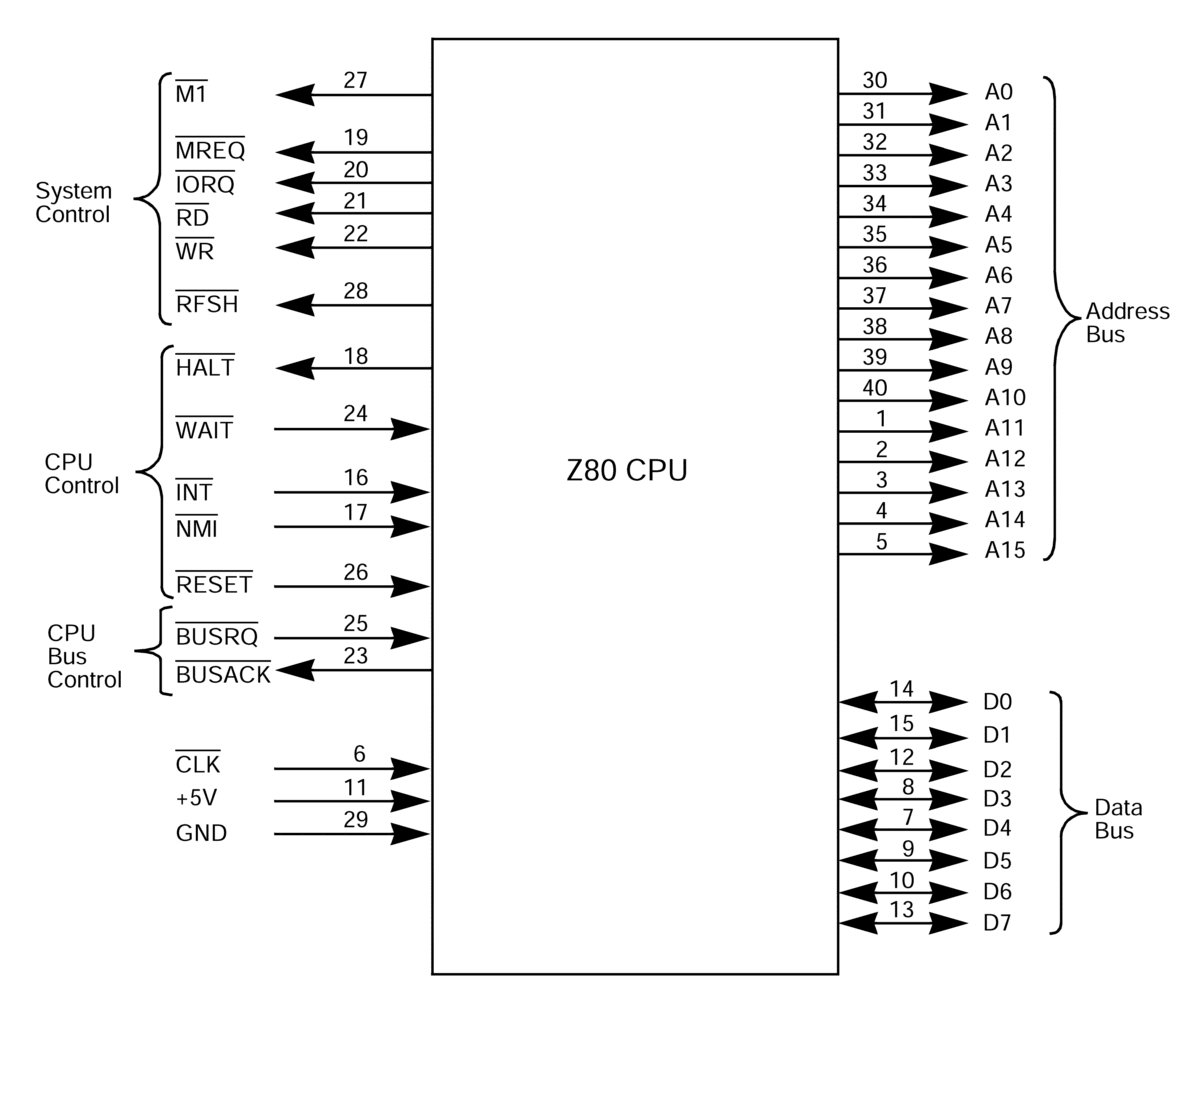
\includegraphics[width=0.5\textwidth]{images/z80.jpg}
\caption{Microprocesor Z80.}
\label{fig:z80}
\end{figure}

\subsubsection{Registrii}
\cite{ref:z80instructions}Procesorul are 10 registrii pe 8 biti,8 din care sunt pentru uz general, si 4 registrii pe 16 biti.
Rolul registrilor:
\begin{itemize}
\item A,B,C,D,E,H,L sunt registrii de uz general pe 8 biti.
\item F este un registru de flaguri.
\item PC este un registru pe 16 biti care contine adresa instructiunii curente.
\item SP este un registru pe 16 biti care contine adresa stivei.
\item IX si IY sunt registrii pe 16 biti folositi pentru indexare.
\item I este un registru pe 8 biti folosit pentru intreruperi.
\item R este un registru pe 8 biti folosit pentru temporizare.
\par \hspace{1em} \textit{Acesta este incrementat cu 1 la fiecare instructiune executata.}
\item AF, BC, DE si HL sunt registrii de uz general pe 16 biti, fiecare fiind format de 2 registrii pe 8 biti.
\end{itemize}
Structura acestora se poate vedea si in Figura \cref{fig:z80registers}.
\begin{figure}[H]
\centering
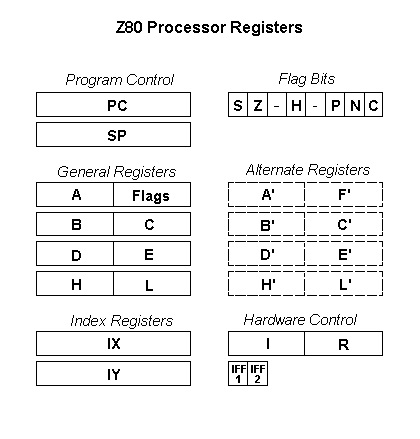
\includegraphics[width=0.5\textwidth]{images/z80registers.jpg}
\caption{Structura registrii Z80. \cite{ref:z80registers}}
\label{fig:z80registers}
\end{figure}

Registrul SP, varful stivei, este initializat cu 0xFFFF, valoarea acestuia scazand la instructiunile de PUSH si crescand la cele de POP

Registrul PC este initializat cu 0x0000.

Structura acestuia se poate vedea si in Tabela \cref{tab:z80flags}.
\begin{table}[h]
\centering
\begin{tabular}{|c|c|c|c|c|c|c|c|c|}
\hline
\textbf{Bit} & 7 & 6 & 5 & 4 & 3 & 2 & 1 & 0 \\
\hline
\textbf{Flag} & S & Z & F5 & H & F3 & P/V & N & C \\
\hline
\end{tabular}
\caption{Z80 Flags}
\label{tab:z80flags}
\end{table}

\subsubsection{Memorie}

Desi microprocesorul are magistrala de date pe 8 biti, acesta foloseste 16 biti pentru adresare. Datorita acestui lucru capacitatea maxima de memorie este de \(2^{16}=65536\) octeti. Aceasta zona de memorie de 64K poate fi separata intre \ac {ROM} si \ac {RAM} in functie de implementare.

Unele periferice in aceste sisteme sunt legate direct la memorie, acest lucru permitand microprocesorului sa comunice cu dispozitive externe prin simple scrieri si citiri din memorie.

Un exemplu de astfel de dispozitiv ar putea fi un ecran extern, fiecare pixel de pe acesta fiind reprezentat de o locatie in memorie, valoarea din aceasta specificand culoarea pixelului.

\subsubsection{Instructiuni}

Modelul oficial al \ac {Z80} contine 158 de instructiuni. Luand in considerare fiecare variatie a acestora, numarul total de instructiuni este de 696.
Instructiunile sunt impartite in 8 categorii principale:
\begin{itemize}
\item Load si Exchange
\item Transfer bloc de date si cautare
\item Aritmetice si logice
\item Rotiri/Shiftari
\item Instructiuni la nivel de bit
\item Jump/Call/Return
\item \ac {IO}
\item Control
\end{itemize}

Instructiunile de tip Load sunt cele care copiaza datele intern intre registrii sau intre registrii si memoria externa.
Toate aceste instructiuni specifica o locatie sursa de unde sa fie copiata valoarea si o destinatie unde sa fie copiata aceasta.
Locatia sursa nu este afectata de aceste instructiuni, aceasta fiind doar citita.
Exemple de asfel de instructiuni sunt cele care copiaza valoarea dintr-un registru in altul "LD A,B" sau cele care copiaza valoarea dintr-o locatie de memorie in registru "LD A,(HL)".

Instructiunile de tip exchange sunt cele care interschimba valorile dintre registrii.

Un set unic de instructiuni de transfer al blocurilor de date sunt include in \ac {Z80}.
Cu o singura instruciune, un bloc din memorie de orice marime poate fi mutat in orice alta locatie din memorie.
Aceste instructiuni sunt foarte folositoare in procesarea sirurilor de caractere.
Cu o singura instructiuni, un bloc intreg de de memorie de orice marime poate fi cautat dupa un anumit byte.
Cand valoarea este gasita sau se ajunge la sfarsitul blocului, instructiunea se opreste automat.
Instructiunile de acest tip permit intreruperile sa fie procesate in timpul executiei lor, astfel incat procesorul nu este blocat pentru perioade lungi de timp.

Instructiunile aritmetice si logice opereaza pe datele stocate in acumulator si alti registrii sau valori din memorie.
Rezultatul operatiei este stocat in acumulator.
De asemenea registrul de flaguri este actualizat in functie de rezultatul operatiei.

Rotate si Shift sunt grupuri de instructiuni care permit registrilor cat si valorilor din memorie sa fie rotite sau shiftate la stanga sau dreapta, cu sau fara carry.

Operatiunile la nivel de bit permit oricarui bit din acumulator, alt registru sau o locatie din memorie sa fie setat, resetat sau testat.

Jump, Call si Return sunt tipuri de instructiuni care transfera executia programului la o alta locatie din memorie.
Aceste instructiuni folosesc mai multe metode diferite de a transfera controlul programului.
Instructiunea Reset este un tip special de Call care permite saltul la doar 8 locatii diferite din memorie.
Alte instructiuni permit incarcarea Program Counter (PC) direct cu o valoare din memorie specificata de HL, IX sau IY.
Aceste instructiuni permit un nivel de control foarte inalt asupra executiei programului.

Instructiunile de \ac {IO} permit un spectru larg de transferuri de date intre microprocesor si dispozitivele externe.
O instructiune de acest tip foloseste ca port in transfer al doilea byte al instructiunii.
Alta instructiune permite portului sa fie specificat de registrul C.
Un avantaj mare in a folosi portul C, este ca permite unei functii sa fie refolosita pentru orice port.
Acest lucru nu ar fi posibil daca portul ar fi specificat de al doilea byte al instructiunii.
O buna caracteristica a acestor instructiuni este ca modifica automat flagurile in functie de rezultatul operatiei.
Din acest motiv nu este necesar sa se faca verificari suplimentare pentru a testa rezultatul operatiei. Exemplu: flagul de semn este setat daca rezultatul operatiei este negativ.

\ac {Z80} include instructiuni care sunt capabile sa mute blocuri intregi de date (pana la 256 byte) automata intre orice port \ac {IO} si memorie
Impreuna cu setul dual de registrii cu scop general, aceste instructiuni faciliteaza transferuri rapide de rate cu dispozitivele externe.

Instructiunile de control sunt instructiuni care controleaza mici aspecte ale microprocesorului.
Unele instructiuni de acest tip sunt cele care activeaza sau dezactiveaza intreruperile, sau cele care controleaza modul de raspuns la intreruperi.

\subsection{Emulator}
Un emulator reprezinta o metoda hardware sau software de a imita un alt tip de sistem de calcul, cum ar fi un procesor, consola sau chiar un intreg calculator.

In cazul acestui lucrari s-a ales un emulator software, acesta fiind mult mai accesibil.

Principala aplicatie a unui emulator este de a rula un program scris pentru o anumita arhitectura pe una complet diferita.

Acest lucru ajuta in mentenanta pe termen lung permitand inlocuirea componentei hardware vechi cu una mai noua fara a necesita software nou.

In cazul curent, deoarece \ac {Z80} este destul de vechi si procurarea acestuia a devenit o problema, in cazul in care microcontrolerul necesita inlocuirea, acesta va putea fi inlocuit cu un Raspberry Pi (sau o alternativa) ruland un emulator.

Pentru realizarea proiectului, emulatorul este necesar sa contina memoria, registrii, si logica necesara pentru decodarea si executarea instructiunilor.

Emularea se va face cat mai apropiat de un Z80 real, acest lucru fiind necesar pentru a asigura ca aplicatiile scrise pentru Z80 vor rula corect.
Pentru asigurarea calitatii si corectitudinii, toate instructiunile Z80 vor fi implementate, acestea fiind testate cu ajutorul unor teste unitare.

Emularea va functiona la nivel de instructiune, acest lucru permitand o monitorizare cat mai buna a executiei programului.
Utilizatorul va avea in fiecare moment control asupra executiei programului, acesta putand pune pauza executiei, modifica registrii sau vizualiza memoria.
Aceste facilitati ar trebui sa ofere un avantaj enorm in depanarea aplicatiilor scrise pentru Z80.
Un asemenea debugger ii va permite programatorului sa vada exact ce se intampla in fiecare moment al executiei programului.

Deoarece se vrea un nivel cat mai inalt de control, memoria emulatorului de asemenea va putea fi configurata.
Zone intregi de memori pot fi alocate ca fiind \ac {ROM} sau \ac {RAM}, sau chiar nealocate.
Deoarece codul va rula in emulator, in cazul accesarii unei zone de memorie nealocate, acest lucru va fi detectat si va fi notifica utilizatorul.

Pentru a simula dispozitivele externe, emulatorul va avea si un sistem de porturi \ac {IO}.
Porturile \ac {IO} in cazul emulatorului, vor fi legate la niste dispozitive virtuale care vor simula dispozitivele reale.
Aceste dispozitive virtuale vor fi configurabile de catre utilizator, acesta putand alege ce dispozitive sa fie simulate si ce porturi sa fie folosite.
Exemplu: Emulatorul va putea simula accesul la un ecran, tastatura sau chiar un dispozitiv de stocare.

O alta caracteristica pe care o va avea emulatorul este cea de extensibilitate.
Emulatorul va fi scris ca o librarie, acesta putand fi inclus in orice alt proiect scris in Rust.
Acest lucru va permite utilizatoriilor sa isi creeze propriile dispozitive compatibile cu emulatorul.
Exemplu: Un utilizator ar putea sa creeze un dispozitiv care sa simuleze un ecran cu o rezolutie mai mare


%\begin{multicols}{2}

%\begin{lstlisting}[language=C++]
%#include <iostream>
%using namespace std;
%
%int main() {
%    cout << "Hello, C++!" << endl;
%    return 0;
%}
%\end{lstlisting}
%\end{multicols}

\subsection{Decizie limbaj de programare}

In procesul de alegere a limbajului de programare, s-au luat in considerare mai multe aspecte, cum ar fi:
:qperformanta, documentatie si securitate.

Performanta este un aspect important, deoarece emulatorul va trebui sa ruleze cat mai fluid si cat mai apropiat de un Z80 real.
Un emulator eficient putand fi capabil sa ruleze in functie de nevoie chiar mai rapid.

Din aceasta cauza a fost preferat un limbaj compilat ce permite un control mai fin asupra memoriei si a resurselor.

Limbaje cum ar fi JavaScript si Python desi capabile, ar avea probleme in a mentine nivelul de performanta necesar unui astfel de emulator.

Un limbaj foarte folosit, mai ales pe embedded este C/C++, acesta fiind considerat a fi printre cele mai rapide.

Alt limbaj care a fost luat in considerare a fost Rust, acesta fiind un limbaj modern,
care oferta acelasi nivel de control si performanta ca C/C++, dar cu un sistem de tipuri mai sigur si mai usor de folosit.

Un mare avantaj al \ac {Rust} este sistemul sau de tipuri si de ownership,
acesta putand preveni multe buguri comune din C/C++ cum ar fi race conditions, memory leaks sau dereferentierea unui pointer null.

\begin{wrapfigure}{r}{0.4\textwidth}
\centering
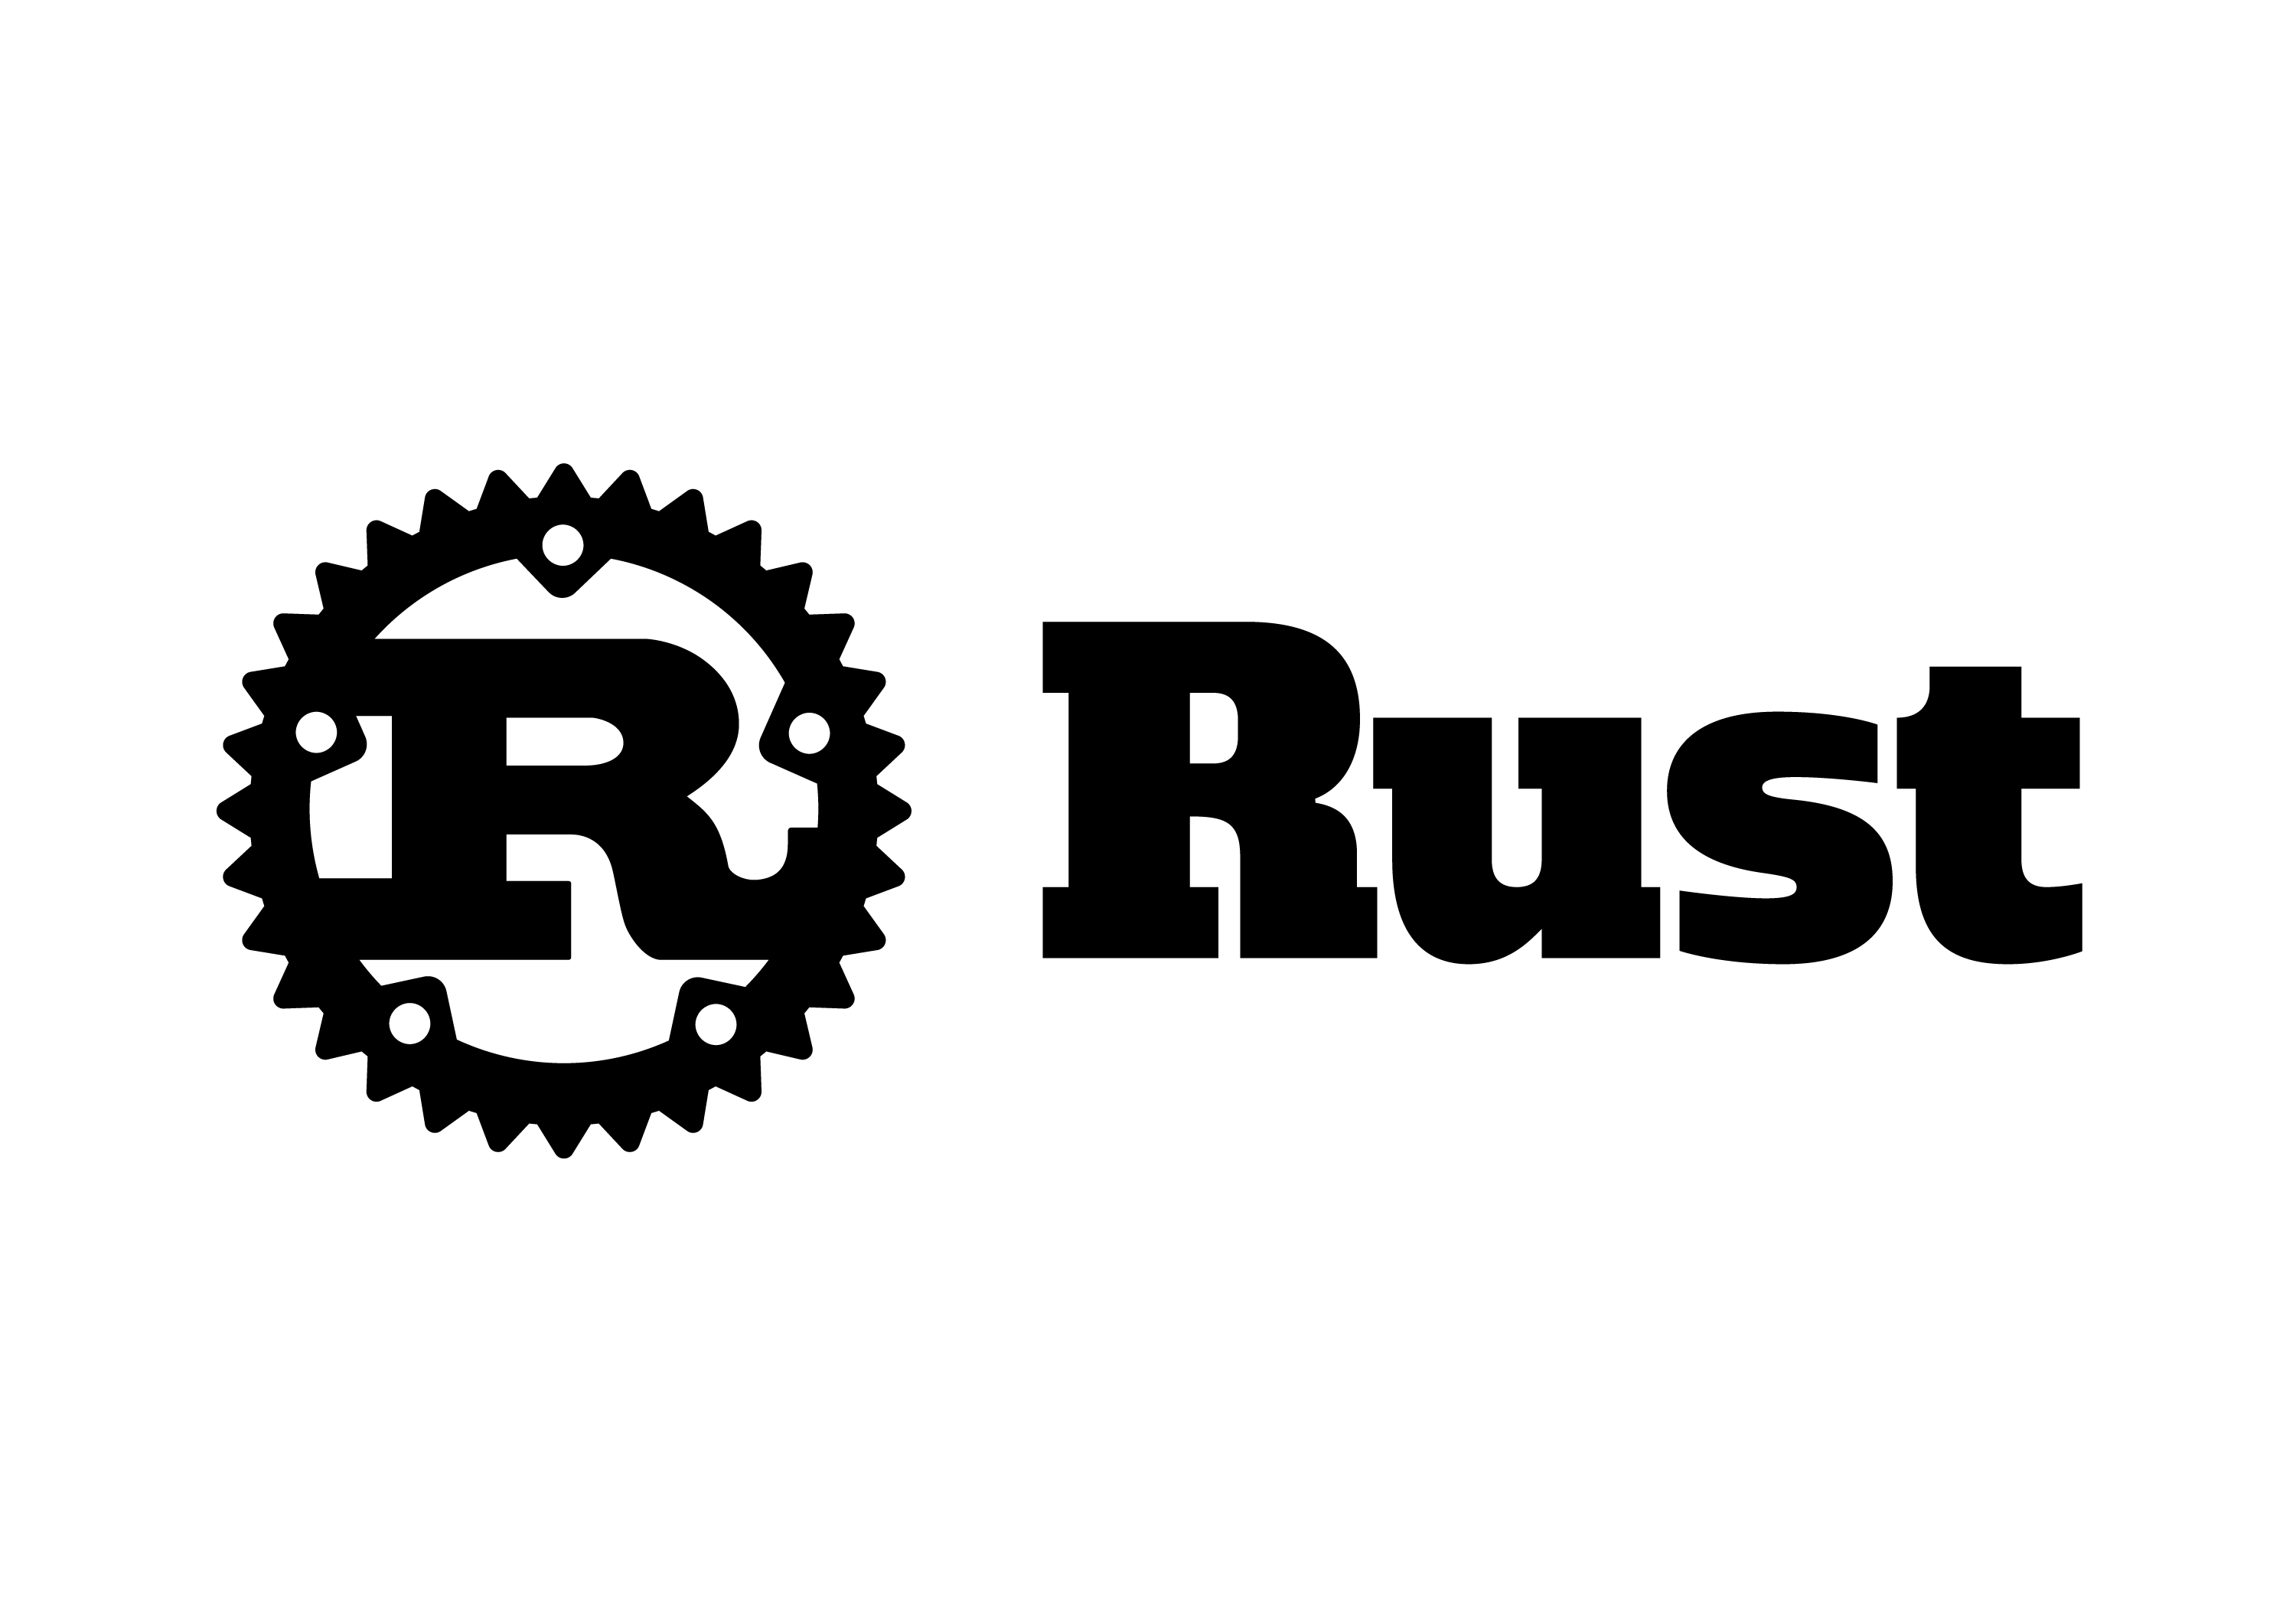
\includegraphics[width=0.4\textwidth]{images/rust_gear_logo.png}
\caption{Logo Rust}
\label{fig:rust-logo}
\end{wrapfigure}

In \ac {Rust} nu exista pointeri null, acest lucru fiind inlocuit de tipul Option<T>,acesta fiind un enum care poate fi Some(T) sau None.

Datorita nivelului ridicat de securitate adus de Rust,
\ac {DARPA} a lansat proiectul TRACTOR, acest proiect are ca tinta transformarea automata a codului C/C++ in Rust.

Un alt motiv din cauza carui \ac {Rust} a fost ales ca limbaj pentru proiect, este faptul ca acesta poate fi compilat cu usurinta in \ac {WASM},
acest lucru va permite rularea aplicatiei in orice browser web modern.

\subsection{Web}

In ultimii ani, aplicatiile web au devenit din ce in ce mai populare, acestea fiind usor de accesat si de folosit.
Un avantaj major al aplicatiilor web este faptul ca acestea pot rula pe orice dispozitiv care are un browser web.
Datorita avansarii rapide in tehnologie, acum se pot gasi pe piata frigidere si masini de spalat care au un browser web, lucru care ar fi fost greu de crezut acum 20 ani.

Un alt avantaj al aplicatiilor web este faptul ca acestea pot fi rulate fara a fi instalate, acest lucru fiind un avantaj major in cazul unui emulator.
Mare parte din emulatoarele existente necesita instalare, acest lucru fiind un inconvenient pentru utilizatorii care nu doresc sau nu pot sa faca acest lucru.
Deoarece aplicatia este rulata din browser, utilizatorul nu risca sa descarce un virus, aplicatia web neavand access direct asupra calculatorului.
Un alt avantaj a creari unei aplicatii web este ca emulatorul va fi capabil sa ruleze pe orice arhitectura de procesor sau sistem de operare, atat timp cat acesta are un browser web modern.

Desi aplicatia web va fi capabila sa functioneze in mod standalone, complet offline, aceasta va putea fi integrata si in alte aplicatii web, oferind un nivel de control mai mare asupra acesteia.

In proiectul curent, va fi de asemenea folosit si un server pentru partea de backend. Desi nu este necesar, acesta este folosit pentru a oferi o experienta mai buna utilizatorului.
Anumite actiuni, cum ar fi compilarea codului C in cod Z80, nefiind posibile in browser, acestea fiind procesate de backend si apoi transmise inapoi catre client.

Contrar multor aplicatii web, aceasta nu va folosi javascript, singura parte de javascript fiind cea care incarca aplicatia \ac {WASM} in browser.
\ac {WASM} a fost ales deoarece este mult mai performant decat javascript, acesta fiind capabil sa ruleze cod mult mai rapid. De asemenea, deoarece fisierele ".wasm" sunt in format binar,
nu text precum javascript, acestea sunt mult mai compacte, ocupand mai putin spatiu si facilitand o incarcare mai rapida a aplicatiei.

\ac {Rust} a fost folosit ca limbaj de programare atat pentru frontend cat si pentru backend.
Folosirea aceluiasi limbaj de programare pe ambele parti, va facilita dezvoltarea si mentenanta aplicatiei.

Serializarea si deserializarea datelor reprezinta procesul prin care structuri de date complexe sunt convertite in format text sau binar, pentru a putea fi transmise pe retea sau salvate pe disk.
In cazul aplicatiei web, serializarea si deserializarea datelor este necesara pentru a putea transmite datele de la client la server si invers.
Pentru aceasta, se va folosi formatul JSON, acesta fiind un format des folosit pentru web, si foarte bine suportat de \ac {Rust}.
Datorita librariei de serializare/deserializare Serde, aceasta operatie este foarte usoara si rapida de realizat.
Toate structurile de date fiind serializabile/deserializabile cu modificari minime.
Acest lucru ne face foarte usoara transmiterea de obiecte intre server si client.

Serverul aplicatiei va avea access la randul sau la o baza de date, aceasta oferind functionalitatile extra doar utilizatorilor logati.
Pentru o securitate cat mai buna, parolele nu vor fi salvate direct in baza de date.
In schimb, acestea vor fi criptate folosind algoritmul de hashing argon2.
Aceasta metoda de criptare este una dintre cele mai sigure, aceasta fiind capabila sa reziste unor atacuri brute force chiar si pe cele mai puternice calculatoare.

De asemenea, un sistem de tokenuri va fi folosit pentru a autentifica utilizatorii.
Acest lucru va permite serverului sa stie daca un utilizator este logat sau nu, fara a fi nevoie de a trimite parola la fiecare request.
Un token unic este creat de server la fiegare logare, acesta fiind trimis inapoi si stocate in browser de catre client.
Server apoi la fiecare request va verifica daca tokenul este valid si daca este, va permite accesul la resursele protejate.

\subsection {Docker}

Docker\cite{ref:docker} este o platformă open-source destinată automatizării procesului de creare, livrare și rulare a aplicațiilor într-un mediu izolat numit container.
Scopul principal al Docker este de a facilita rularea aplicațiilor într-un mod reproductibil și portabil, indiferent de sistemul de operare gazdă.
\paragraph{Arhitectura Docker}

\begin{figure}[H]
\centering
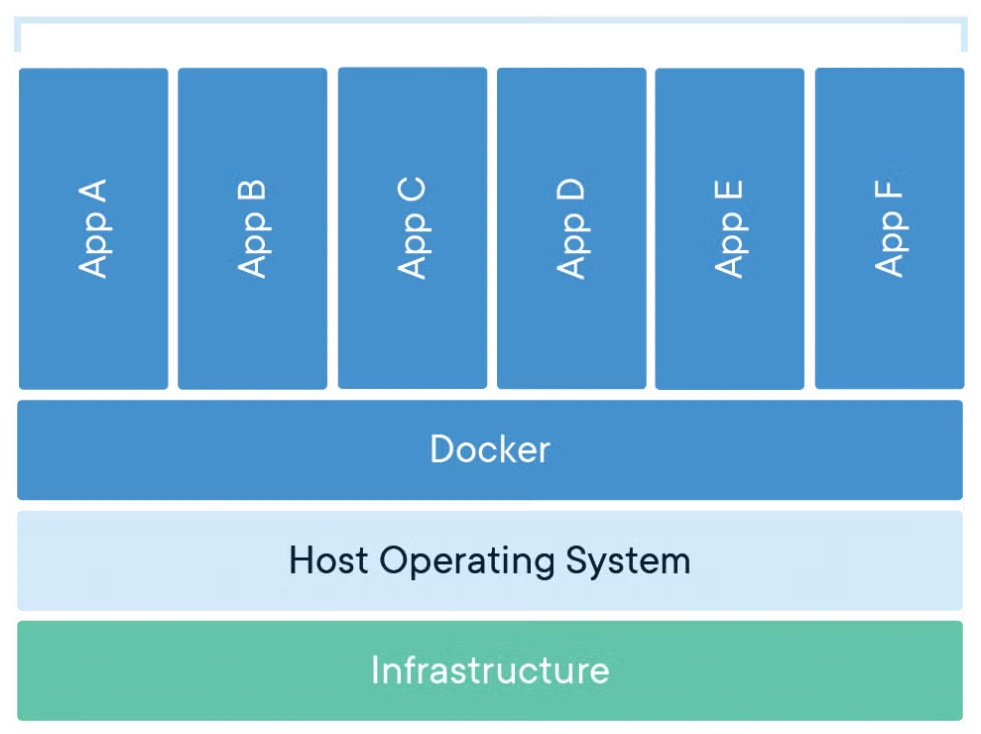
\includegraphics[width=0.6\textwidth]{images/dockerstructure}
\caption{Structura Docker.}
\label{fig:containerstructure}
\end{figure}

Un container Docker este o instanță rulabilă a unei imagini (image) Docker.
Imaginile sunt fișiere read-only ce conțin tot ceea ce este necesar pentru rularea unei aplicații: codul sursă, biblioteci, instrumente de sistem, fișiere de configurare și un runtime.
Aceste imagini sunt construite pornind de la un fișier special denumit \code{Dockerfile}, care conține instrucțiuni pas cu pas pentru configurarea mediului de execuție.

Fiecare container este izolat de celelalte și de sistemul gazdă, având propriile procese, rețele, sisteme de fișiere și spații de nume.
Spre deosebire de mașinile virtuale tradiționale, containerele împart același kernel al sistemului de operare, ceea ce le face mult mai eficiente în termeni de resurse.

Arhitectura Docker este compusă din mai multe componente-cheie:

\begin{itemize}
\item \textbf{Docker Engine} – serviciul care rulează pe sistemul gazdă și permite crearea, rularea și gestionarea containerelor.
\item \textbf{Imagini Docker (Docker Images)} – șabloane read-only folosite pentru a crea containere.
\item \textbf{Registrul Docker (Docker Registry)} – un sistem de tip repository pentru stocarea și partajarea imaginilor (ex: Docker Hub, GitHub Container Registry).
\item \textbf{Containere (Containers)} – instanțe izolate ale imaginilor, ce rulează aplicația propriu-zisă.
\item \textbf{Volume} – mecanism de persistență a datelor între mai multe rulări de containere.
\item \textbf{Rețele Docker (Docker Networks)} – oferă containerelor capacitatea de a comunica între ele sau cu lumea exterioară.
\end{itemize}

\paragraph{Avantajele utilizării Docker}

Docker oferă numeroase beneficii în dezvoltarea și livrarea aplicațiilor:

\begin{itemize}
\item \textbf{Portabilitate} – o aplicație containerizată poate fi rulată identic pe orice sistem cu Docker instalat, indiferent de mediul de execuție.
\item \textbf{Eficiență} – spre deosebire de mașinile virtuale, containerele au un overhead foarte redus și pornesc în câteva milisecunde.
\item \textbf{Izolare} – fiecare container rulează într-un spațiu izolat, ceea ce crește securitatea și stabilitatea aplicației.
\item \textbf{Scalabilitate} – Docker este integrat ușor cu sisteme de orchestrare precum Kubernetes sau Docker Swarm, permițând scalarea automată a aplicațiilor.
\item \textbf{Consistență} – mediile de dezvoltare, testare și producție pot fi standardizate, reducând riscul de erori cauzate de diferențe de configurație.
\end{itemize}

\paragraph{Docker în context DevOps și CI/CD}

În cadrul metodologiilor DevOps, Docker joacă un rol esențial în crearea unor pipeline-uri de livrare continuă (CI/CD).
De exemplu, codul sursă poate fi testat, construit și containerizat automat folosind instrumente precum GitHub Actions, GitLab CI, Jenkins sau Azure Pipelines.
Astfel, la fiecare commit, o nouă imagine poate fi generată, testată automat și livrată într-un mediu de staging sau producție.

\paragraph{Persistența datelor și comunicația între containere}

Pentru aplicațiile care necesită stocarea de date persistente, Docker oferă volume, care sunt directoare montate din exteriorul containerului.
Acestea permit salvarea datelor și după ce un container este oprit sau recreat.

Comunicarea între containere este posibilă prin rețele Docker dedicate.
Astfel, o aplicație web rulată într-un container poate comunica direct cu o bază de date aflată într-un alt container, fără a expune aceste servicii în exterior.

\begin{lstlisting}[language=docker,caption={Exemplu Dockerfile},label={lst:dockerfile}]
FROM rust:1.52
WORKDIR /usr/src/myapp
COPY . .
RUN cargo build --release
CMD ["cargo", "run"]
\end{lstlisting}

În exemplul din \cref{lst:dockerfile}, se construiește o imagine Docker pentru o aplicație Rust.
Aceasta este compilată în mod optimizat (\code{--release}) și apoi rulată automat la pornirea containerului.

\subsection{Kubernetes}

\ac {K8s} este o platformă open-source pentru orchestrarea containerelor, care permite gestionarea automată a aplicațiilor containerizate la scară largă. Unul dintre principalele sale scopuri este de a facilita implementarea, scalarea și gestionarea aplicațiilor în containere, asigurându-se că acestea rulează în mod fiabil și eficient.
Pe baza acestei platofrme se pot face deploy-uri automate, se pot gestiona resursele și se pot monitoriza aplicațiile într-un mod centralizat.

\begin{itemize}
    \item \textbf{Master Node}: Este responsabil pentru gestionarea întregului cluster. Include componente precum \textit{API Server}, \textit{Scheduler} și \textit{Controller Manager}.
    \item \textbf{Worker Nodes}: Acestea găzduiesc aplicațiile containerizate. Fiecare nod conține un \textit{kubelet}, care comunică cu Master Node, și un \textit{Container Runtime} pentru rularea containerelor.
    \item \textbf{etcd}: O bază de date distribuită care stochează toate datele de configurare ale clusterului.
    \item \textbf{Controller Manager}: Gestionează controlerele care monitorizează starea clusterului și efectuează acțiuni corective.
    \item \textbf{Scheduler}: Atribuie workload-urile (pod-urile) nodurilor disponibile, ținând cont de resursele acestora.
\end{itemize}

\paragraph{Concepte cheie}
\begin{itemize}
    \item \textbf{Pod}: Cea mai mică unitate de lucru din \ac {K8s}, care conține unul sau mai multe containere ce împart aceeași rețea și spațiu de stocare.
    \item \textbf{Service}: O abstracție care expune un set de pod-uri ca un serviciu de rețea.
    \item \textbf{Deployment}: Un obiect care definește modul în care aplicațiile sunt implementate și gestionate, permițând actualizări și rollback-uri.
    \item \textbf{Namespace}: Un mecanism de izolare logică pentru organizarea resurselor dintr-un cluster.
    \item \textbf{ConfigMap și Secret}: Resurse utilizate pentru a gestiona configurările aplicațiilor și datele sensibile, cum ar fi parolele.
\end{itemize}

\paragraph{Avantajele utilizării \ac {K8s}}
\begin{itemize}
    \item \textbf{Scalabilitate automată}: Kubernetes poate scala automat aplicațiile în funcție de cerințele de resurse.
    \item \textbf{Toleranță la erori}: Asigură disponibilitatea aplicațiilor prin repornirea automată a pod-urilor defecte și redistribuirea acestora pe noduri sănătoase.
    \item \textbf{Portabilitate}: Aplicațiile containerizate pot fi rulate pe orice infrastructură care suportă Kubernetes, fie că este vorba de cloud public, privat sau on-premises.
    \item \textbf{Gestionare declarativă}: Configurațiile sunt definite într-un mod declarativ, utilizând fișiere YAML sau JSON.
    \item \textbf{Integrare cu DevOps}: Kubernetes se integrează ușor cu pipeline-urile CI/CD, facilitând livrarea continuă a aplicațiilor.
\end{itemize}

\paragraph{Flux de lucru tipic}
Un flux de lucru tipic în Kubernetes implică următorii pași:
\begin{enumerate}
    \item Crearea unui fișier de configurare YAML pentru resursele necesare (Pod, Deployment, Service etc.).
    \item Aplicarea configurației folosind comanda \texttt{kubectl apply}.
    \item Monitorizarea stării clusterului și a resurselor utilizând comanda \texttt{kubectl get}.
    \item Scalarea aplicațiilor folosind comanda \texttt{kubectl scale}.
    \item Actualizarea aplicațiilor prin modificarea configurației și reaplicarea acesteia.
\end{enumerate}

Kubernetes a devenit standardul de facto pentru orchestrarea containerelor, oferind un ecosistem robust și extensibil pentru gestionarea aplicațiilor moderne.

\subsection{Version Control (Git)}

Controlul versiunilor este un sistem esențial în gestionarea codului sursă pe parcursul dezvoltării software. Acesta permite urmărirea modificărilor aduse fișierelor de-a lungul timpului, facilitând gestionarea mai multor versiuni ale unui proiect, colaborarea între dezvoltatori și asigurarea integrității și consistenței codului sursă.

Git este un sistem de control al versiunilor distribuit, creat de Linus Torvalds în 2005 pentru a sprijini dezvoltarea kernel-ului Linux. Spre deosebire de sistemele de control al versiunilor centralizate, Git oferă fiecărei instanțe a depozitului (repository) o copie completă a întregii istorii a proiectului. Acest lucru înseamnă că fiecare dezvoltator poate lucra în mod independent și local, iar modificările pot fi sincronizate ulterior cu depozitul central.

Principalele caracteristici ale Git sunt:

\begin{itemize}
\item \textbf{Sistem distribuit}: Fiecare dezvoltator are o copie completă a întregului proiect, inclusiv istoricul său, pe mașina locală. Aceasta permite lucrul offline și îmbunătățește performanța.
\item \textbf{Măcinarea și ramificarea ușoară}: Git permite crearea de ramuri (branches) ușor, care sunt esențiale pentru dezvoltarea paralelă a funcționalităților noi sau pentru testarea unor idei.
\item \textbf{Fazele fluxului de lucru}: Modificările sunt gestionate prin trei zone: Working Directory, Staging Area și Repository. Aceste zone permit dezvoltatorilor să adauge, să verifice și să stocheze modificările înainte de a le trimite în depozitul central.
\item \textbf{Performanță ridicată}: Git este extrem de rapid la operații comune, cum ar fi comiterea, schimbarea ramurilor sau unirea acestora.
\item \textbf{Securitate}: Git folosește un sistem de hash criptografic (SHA-1) pentru a verifica integritatea fișierelor și istoricului, protejând astfel datele împotriva corupției.
\end{itemize}

Un flux de lucru tipic cu Git implică următoarele etape:
\begin{enumerate}
\item \textbf{Clonarea depozitului}: Dezvoltatorul își clonează depozitul central pe mașina locală folosind comanda \code{git clone}.
\item \textbf{Crearea unei ramuri}: Dezvoltatorul creează o ramură de lucru pentru a dezvolta o caracteristică sau a rezolva o problemă.
\item \textbf{Comiterea modificărilor}: După ce au fost efectuate modificări, dezvoltatorul le adaugă în zona de stagiu (staging area) folosind comanda \code{git add}, iar apoi le salvează în depozitul local cu comanda \code{git commit}.
\item \textbf{Împingerea modificărilor}: După ce modificările sunt comise, acestea pot fi trimise la depozitul central folosind comanda \code{git push}.
\item \textbf{Îmbinarea modificărilor}: Dacă mai mulți dezvoltatori lucrează pe aceeași ramură, modificările lor pot fi combinate folosind comanda \code{git merge}.
\end{enumerate}

Comparativ cu alte sisteme de control al versiunilor, cum ar fi SVN (Subversion), Git oferă o mai mare flexibilitate și performanță. De exemplu, SVN este un sistem de control al versiunilor centralizat, ceea ce înseamnă că există un depozit central unde toate modificările sunt stocate. Git, pe de altă parte, este un sistem distribuit, permițând fiecărui dezvoltator să aibă o copie completă a întregului proiect, ceea ce îl face mai eficient în lucrul cu proiecte mari și echipe distribuite. Git este, de asemenea, mult mai rapid în gestionarea ramurilor și în combinarea modificărilor, fiind ideal pentru dezvoltarea de software agil.

\subsection{Cloud Computing}

Cloud Computing reprezintă livrarea de servicii IT, cum ar fi stocare, procesare, baze de date, rețele și software, prin intermediul internetului („cloud”), oferind acces la resurse scalabile și flexibile fără a necesita investiții în infrastructură fizică.

\paragraph{Modele de servicii}
Cloud Computing este clasificat în trei modele principale de servicii:
\begin{itemize}
    \item \textbf{\ac {IaaS}}: Oferă infrastructură virtualizată, cum ar fi servere, stocare și rețele. Exemple: Amazon EC2, Microsoft Azure Virtual Machines.
    \item \textbf{\ac {PaaS}}: Oferă un mediu de dezvoltare și implementare pentru aplicații, eliminând necesitatea gestionării infrastructurii. Exemple: Google App Engine, Heroku.
    \item \textbf{\ac {SaaS}}: Oferă aplicații software accesibile prin internet, fără a necesita instalare locală. Exemple: Google Workspace, Microsoft 365.
\end{itemize}

\paragraph{Modele de implementare}
Există mai multe modele de implementare a cloud-ului:
\begin{itemize}
    \item \textbf{Cloud public}: Resursele sunt partajate între mai mulți utilizatori și sunt gestionate de un furnizor terț. Exemple: \ac {AWS} , \ac {GCP}.
    \item \textbf{Cloud privat}: Resursele sunt dedicate unei singure organizații, oferind un control mai mare asupra datelor și securității.
    \item \textbf{Cloud hibrid}: Combină cloud-ul public și privat, permițând organizațiilor să beneficieze de flexibilitate și scalabilitate.
    \item \textbf{Cloud comunitar}: Resursele sunt partajate între organizații cu interese comune, cum ar fi instituțiile guvernamentale.
\end{itemize}

\paragraph{Avantajele Cloud Computing}
\begin{itemize}
    \item \textbf{Scalabilitate}: Resursele pot fi ajustate rapid în funcție de cerințele utilizatorului.
    \item \textbf{Costuri reduse}: Elimină necesitatea investițiilor în hardware și întreținere.
    \item \textbf{Accesibilitate}: Serviciile sunt accesibile de oriunde, atâta timp cât există o conexiune la internet.
    \item \textbf{Fiabilitate}: Majoritatea furnizorilor de cloud oferă redundanță și backup automat pentru a asigura disponibilitatea serviciilor.
    \item \textbf{Securitate}: Furnizorii de cloud implementează măsuri avansate de securitate pentru protejarea datelor.
\end{itemize}

\paragraph{Google Cloud Platform}
a fost ales datorită serviciilor sale robuste și a integrării ușoare cu tehnologiile necesare. \ac {GCP} oferă o infrastructură scalabilă și flexibilă, care a permis implementarea eficientă a aplicației.

\begin{itemize}
    \item \textbf{Docker Engine}: GCP oferă suport nativ pentru containere prin Google Kubernetes Engine (GKE) și alte servicii, facilitând rularea aplicației containerizate. Docker Engine a fost esențial pentru izolarea și gestionarea mediului de execuție al aplicației.
    \item \textbf{Managementul certificatelor SSL}: GCP include servicii precum \textit{Certificate Manager}, care simplifică gestionarea certificatelor SSL. Acest lucru a asigurat o conexiune securizată între utilizatori și aplicație, respectând standardele moderne de securitate.
    \item \textbf{Scalabilitate automată}: GCP a permis scalarea automată a resurselor în funcție de cerințele aplicației, reducând costurile și asigurând performanța optimă.
    \item \textbf{Integrare cu CI/CD}: GCP s-a integrat ușor cu pipeline-urile de livrare continuă, facilitând implementarea rapidă a actualizărilor și testarea automată.
\end{itemize}

\paragraph{Provocări și limitări}
\begin{itemize}
    \item \textbf{Confidențialitatea datelor}: Datele stocate în cloud pot fi vulnerabile la acces neautorizat, dar GCP oferă măsuri avansate de securitate pentru a minimiza riscurile.
    \item \textbf{Dependența de furnizor}: Migrarea către alt furnizor poate fi dificilă, dar flexibilitatea oferită de GCP a redus această preocupare.
\end{itemize}

Google Cloud Platform a oferit toate instrumentele necesare pentru a implementa și gestiona proiectul într-un mod eficient și sigur, contribuind semnificativ la succesul acestuia.

\clearpage
\section{Implementare}
\subsection{Librarie emulator}
Implementarea emulatorului a fost realizata in limbajul de programare Rust, acesta fiind un limbaj modern, rapid si sigur. Deoarece se doreste o modularitate cat mai mare si posibilitatea de a integra proiectul in altele, nucleul emulatorului a fost realizat ca o librarie.
Libraria in sine va contine toate structurile necesare (\code{Emulator}, \code{CPU}, \code{Io} ...etc), cat si implementarea acestora. Impachetand nucleul emulatorului intr-o librarie permite utilizatorilor sa o extinda, cum ar fi sa isi creeze propri dispozitive virtuale sau sa adauge suport pentru alte procesoare.

\subsubsection{Structuri de date}

Pentru crearea emulatorului diferite structuri de date au fost create, unele din acestea imitand componente din realitete (memorie, rom, ram, Z80 ...etc), altele fiind structuri de date care ajuta la implementarea acestora (ex: ExecutableInstruction).

\paragraph{\code{Emulator}} Structura ce va coordona executia procesorului, memoriei si a sistemului IO

\begin{lstlisting}[language=Rust,caption={Structura Emulator},label={lst:emulator_struct}]
pub struct Emulator<T: Cpu> {
    pub memory: Memory,
    pub cpu: T,
    pub breakpoints: Vec<u16>,
    pub io: IO,
    pub cycle_counter: usize,
    pub instruction_counter: usize,
}
\end{lstlisting}

Aceasta structura va contine alte trei structuri: \code{Memory}, \code{Cpu} si \code{IO}. Deoarece emulatorul se vrea cat mai extensibil, structura procesorului nu este una fixa, orice structura de date care implementeaza traitul \code{Cpu} va putea fi folosita. Un mare avantaj al acestui lucra este ca permite implementarea pe viitor a mai multor arhitecturi de procesor.

Pentru a fi capabili sa monitorizam executia programului, in structura \code{Emulator} a fost adaugat un vector de breakpoints. Acestea vor fi folosite pentru a opri executia programului la o anumita adresa de memorie aleasa de utilizator.

Deoarece se doreste o monitorizare cat mai amanunita, aici se va contoriza si numarul de intructiuni executate cat si cel de ciclii executati.

Principala functie care va fi folosita in aceasta structura va fi cea de step \cref{lst:emulator_step}

\begin{lstlisting}[language=Rust,caption={Functia step a emulatorului},label={lst:emulator_step}]
pub fn step(&mut self) -> Result<Box<dyn ExecutableInstruction<T>>, String> {
    if self.cpu.halted() {
        return Err("CPU is halted".to_string());
    }
    self.memory.clear_changes();
    let instruction = self.cpu.step(&mut self.memory, &mut self.io);
    self.io.step();
    if let Ok(instruction) = &instruction {
        self.cycle_counter += instruction.common().cycles as usize;
        self.instruction_counter += 1;
    }
    instruction
}
\end{lstlisting}
Aceasta functie cand va fi apelata va emula executia a unei singure instructiuni. Acest lucru este facut prin a apela instructiunea de step a structurii \code{Cpu}. Cand se va face acest apel, controlul memoriei si al \code{IO} va fi momentan pasat catre functia apelata. Dupa executarea functiei, contoarele vor creste corespunzator.

\paragraph{\code{Memory}} Memoria emulatorului

Aceasta structura \cref{lst:memory_struct} reprezinta intreaga memorie accesibila de emulator.

\begin{lstlisting}[language=Rust,caption={Structura Memorie},label={lst:memory_struct}]
pub struct Memory {
    data: Vec<Box<dyn MemoryDevice>>,
    changes: Option<Vec<u16>>,
    readcallback: Option<fn(u16, u8)>,
    writecallback: Option<fn(u16, u8)>,
}
\end{lstlisting}

Memoria permite setarea unor functii de callback apelate la fiecare citire sau scriere. Acesst lucru putand fi util utilizatorului, daca doreste anumite actiuni sa se intample doar la scrieri sau citiri din memorie.

In proiectarea memoriei initial s-a mers pe idea de a crea un vector de 65536 valori a cate un byte. Dupa mai multa experimentare, aceasta s-a dovedit a fi insuficienta deoarece facea maparea dispozitivelor \code{IO} in memorie dificila. Din acest motiv, structura Memory contine un vector de structuri ce implementeaza \code{MemoryDevice}.
Structurile de baza aduse de emulator care implementeaza \code{MemoryDevice} sunt structurile \code{ROM} si \code{RAM}, acestea emuland un ROM si un RAM adevarat. Pe langa ROM/RAM, pot fi create si alte dispozitive mapate la memorie cum ar fi monitoare, senzori ...etc.
Deoarece structura \code{Memory} este facuta din unul sau mai multe \code{MemoryDevice}, acest lucru permite o mapare a memoriei foarte dinamica si adaptiva in functie de preferinte. Un exemplu de initializare a memoriei se poate vedea in \cref{lst:memory-init-ex} unde prima zona de 0x4000 bytes este ROM iau urmatoarea zona de 0xC000 va fi RAM, aceasta mapare ocupand toata zona de memorie accesibila \cref{tab:memory-mapping-ex}.
\begin{lstlisting}[language=Rust,caption={Exemplu initializare memorie},label={lst:memory-init-ex}]
let mut mem = Memory::new();
mem.add_device(Box::new(memdevices::ROM::new(0x4000)));
mem.add_device(Box::new(memdevices::RAM::new(0xC000)));
\end{lstlisting}

\begin{table}[H]
\centering
\begin{tabular}{|c|c|c|c|}
\hline
\textbf{Adresă de început} & \textbf{Adresă de sfârșit} & \textbf{Tip memorie} & \textbf{Dimensiune} \\
\hline
\texttt{0x0000} & \texttt{0x3FFF} & ROM & \texttt{0x4000} (16 KiB) \\
\hline
\texttt{0x4000} & \texttt{0xFFFF} & RAM & \texttt{0xC000} (48 KiB) \\
\hline
\end{tabular}
\caption{Exemplu mapare memorie}
\label{tab:memory-mapping-ex}
\end{table}

Memoria de asemenea tine un record al modificarilor aduse acesteia, acest lucru fiind util in cazul in care utilizatorul doreste sa vada ce locatii din memorie au fost modificate dupa executarea unei instructiuni.

Implementarea unui dispozitiv propriu de memorie este foarte simpla, singurele functii necesare pentru implementarea acesteia fiind \code{size}, \code{read\_8}, \code{write\_8} si \code{write\_8\_force}. Functia \code{write\_8\_force} face un lucru care normal nu este posibil in realitate, scrierea unei valori cu forta chiar daca acest lucru normal nu ar fi permis, cum ar fi in \code{ROM}.
In \ref{lst:rom-struct} se poate observa cum este implementata structura \code{ROM}, aceasta fiind la baza un vector de bytes, functia \code{size} returnand marimea acestuia si \code{read\_8}, \code{write\_8}, \code{write\_8\_force} scriind valori in al. Deoarece normal scrierea in \code{ROM} este normal imposibila, functia \code{write\_8} va returna o erroare \code{MemoryWriteError::ReadOnly}, in timp ce \code{write\_8\_force} va scrie in ROM fara a verifica daca acest lucru este permis sau nu. Acest lucru este util si faciliteaza depanarea aplicatiilor, permitand utilizatorului sa scrie in \code{ROM} pentru a modifica valorile din acesta.
Pentru un nivel inalt de siguranta la citiri si scrieri se face o verificare a adresei, aceasta fiind verificata sa nu depaseasca dimensiunea memoriei. In cazul in care acest lucru se intampla, se va returna o eroare \code{MemoryRWCommonError::OutOfBounds}.
Pentru ca dorim sa fim capabili sa clonam structura \code{ROM} in cazul in care este nevoie, aceasta structura va implementa si traitul \code{Clone}. Acesta facand orice structura capabila de a fi clonata automat, daca toate structurile din interiorul ei sunt de asemenea capabile de a fi clonate.
Crearea unui \code{ROM} se face prin functia \code{new}, aceasta primind ca parametru dimensiunea dorita a \code{ROM}-ului. Aceasta functie va returna un \code{ROM} cu dimensiunea dorita, initializat cu 0x00 in fiecare locatie de memorie. Pe langa aceasta, deoarece este implementat traitul \code{From<Vec<u8>>}, \code{ROM}-ul poate fi creat si dintr-un vector de bytes.

\begin{lstlisting}[language=Rust,caption={Structura ROM},label={lst:rom-struct}]
#[derive(Debug, Clone)]
pub struct ROM {
    data: Vec<u8>,
}

impl ROM {
    pub fn new(size: usize) -> ROM {
        ROM {
            data: vec![0; size],
        }
    }
}

impl MemoryDevice for ROM {
    fn size(&self) -> usize {
        self.data.len()
    }
    fn read_8(&self, addr: u16) -> Result<u8, MemoryReadError> {
        match self.data.get(addr as usize) {
            None => Err(MemoryRWCommonError::OutOfBounds(addr).into()),
            Some(val) => Ok(*val),
        }
    }
    fn write_8(&mut self, addr: u16, _: u8) -> Result<(), MemoryWriteError> {
        Err(MemoryWriteError::ReadOnly(addr))
    } 

    fn write_8_force(&mut self, addr: u16, data: u8) 
    -> Result<(), MemoryWriteError> {
        let val = self
        .data
        .get_mut(addr as usize)
        .ok_or(MemoryRWCommonError::OutOfBounds(addr))?;
        *val = data;
        Ok(())
    }
}

impl From<Vec<u8>> for ROM {
    fn from(data: Vec<u8>) -> ROM {
        ROM { data }
    }
}
\end{lstlisting}

Singura diferenta in structura \code{RAM} este ca aceasta implementeaza alta functie de scriere, \code{write\_8} va avea aceeasi implementare ca \code{write\_8\_force}, permițând scrierea.

\paragraph{\code{CPU}} Structura ce va contine registrii si instructiunile procesorului

\code{Cpu} este definit ca un trait \cref{lst:cpu_trait} care reprezinta un microprocesor, acest lucru permitand ca orice structura care implementeaza acest trait sa fie folosita in emulator.
\begin{lstlisting}[language=Rust,caption={Trait CPU},label={lst:cpu_trait}]
pub trait Cpu:
Send + Copy + Clone + Default + Serialize + for<'a> Deserialize<'a> {
    fn step(&mut self, memory: &mut Memory, io: &mut IO,)
    -> Result<Box<(dyn ExecutableInstruction<Self>)>, String>;
    fn parser(&self) -> &dyn InstructionParser<Self>;
    fn registers(&self) -> AllRegisters;
    fn registers_mut(&mut self) -> AllMutRegisters;
    fn pc(&self) -> u16;
    fn halted(&self) -> bool;
    fn set_halted(&mut self, halted: bool);
}
\end{lstlisting}
Orice structura ce implementeaza toate functiile traitului \code{Cpu} va putea fi folosita ca procesor pentru emulator. Principala implementare prezentata in proiect a acestui trait este pentru structura \code{Z80}, functia de step a acestuia fiind vizibila in \cref{lst:z80_step}
\begin{lstlisting}[language=Rust,caption={Functia step Z80},label={lst:z80_step}]
fn step(&mut self, memory: &mut Memory, io: &mut IO,)
-> Result<Box<(dyn ExecutableInstruction<Self>)>, String> {
    let res = self.handle_interrupt(memory, io)?;
    let mut instruction: Box<dyn ExecutableInstruction<Z80>> = match res {
        Some(instruction) => instruction,
        None => parser::Z80_PARSER
        .ins_from_machinecode(memory, self.registers.pc)
        .map_err(|e| e.to_string())?,
    };
    instruction.execute(memory, self, io)?;
    let common = instruction.common();
    self.registers.r = self.registers.r.wrapping_add(1) % 0x80;
    if common.increment_pc {
    let inst_length = common.length;
    let new_pc = self.registers.pc.wrapping_add(inst_length);
    self.registers.pc = new_pc;
}
Ok(instruction)
}
\end{lstlisting}

Aceasta functie va verifica prima oara daca trebuie sa se intample o intrerupere, in caz contrar instructiunea din PC va fi decodata. Dupa decodarea instructiunii registrul ascuns R va fi incrementat. De asemenea, daca este cazul, si registrul PC va creste.

\paragraph{\code{Z80Registers}} Structura reprezinta registrii procesorului Z80

In aceasta structura \cref{lst:z80registers-struct} sunt reprezentati toti registrii prezenti intr-un Z80. Pentru a reprezenta cele doua grupuri de registrii cu scop general a fost folosita alta structura \code{GPByteRegisters} \cref{lst:gpbyteregisters-struct}. Aceasta structura contine 8 registrii de cate un byte. De asemenea, in aceasta structura se afla si structura cu flag-urile procesorului, acestea fiind reprezentate prin structura \code{Flags} \cref{lst:flags-struct}.

\begin{lstlisting}[language=Rust,caption={Structura Z80Registers},label={lst:z80registers-struct}]
pub struct Z80Registers {
    pub gp: GPByteRegisters,
    pub gp_alt: GPByteRegisters,
    pub ix: u16,
    pub iy: u16,
    pub i: u8,
    pub r: u8,
    pub sp: u16,
    pub pc: u16,
}
\end{lstlisting}

\code{GPByteRegisters} \cref{lst:gpbyteregisters-struct} reprezinta 8 registrii de cate un byte, accesibili prin \code{a}, \code{b}, \code{c}, \code{d}, \code{e}, \code{h}, \code{l}.
Deoarece se doreste un nivel cat mai inalt de accessibilitate, prin implementarea traitului \code{Deref} structura \code{GPByteRegisters} poate fi dereferentiata si ca \code{GPWordRegisters}, permitand accesul la registrii de cate 2 bytes prin \code{bc}, \code{de}, \code{hl}.

\begin{lstlisting}[language=Rust,caption={Structura GPByteRegisters},label={lst:gpbyteregisters-struct}]
pub struct GPByteRegisters {
    pub f: Flags,
    pub a: u8,
    pub c: u8,
    pub b: u8,
    pub e: u8,
    pub d: u8,
    pub l: u8,
    pub h: u8,
}

pub struct GPWordRegisters {
    pub af: u16,
    pub bc: u16,
    pub de: u16,
    pub hl: u16,
}

impl Deref for GPByteRegisters {
    type Target = GPWordRegisters;
    fn deref(&self) -> &Self::Target {
        unsafe { std::mem::transmute(self) }
}
\end{lstlisting}

\begin{table}[h!]
\centering
\begin{tabular}{|l|c|c|c|c|c|c|c|c|}
\hline
\textbf{Structura} & \textbf{Byte 0} & \textbf{Byte 1} & \textbf{Byte 2} & \textbf{Byte 3} & \textbf{Byte 4} & \textbf{Byte 5} & \textbf{Byte 6} & \textbf{Byte 7} \\
\hline
\texttt{GPByteRegisters} & f & a & c & b & e & d & l & h \\
\hline
\texttt{GPWordRegisters} & \multicolumn{2}{c|}{af} & \multicolumn{2}{c|}{bc} & \multicolumn{2}{c|}{de} & \multicolumn{2}{c|}{hl} \\
\hline
\end{tabular}
\caption{Suprapunerea structuriilor \code{GPByteRegisters} si \code{GPWordRegisters} in memorie}
\end{table}

Pentru a face dereferentierea de la \code{GPByteRegisters} la \code{GPWordRegisters} am fost nevoiti sa facem o operatiune unsafe, aceasta fiind necesara deoarece compilerul Rust considera nesigura aceasta transformare intre structuri. Motivul pentru care este sigura in cazul prezent este ca suntem siguri de dimensiunile structurilor si felul cum acestea sunt compatibile.
Ambele structuri vor avea aceasi reprezentare binara, singura diferenta fiind felul in care sunt accesate datele. Din acest motiv una poate fi transformata in alta fara a fi nevoie de o copiere a datelor.

Structura \code{Flags} \cref{lst:flags-struct} este un bitfield, acest lucru pentru a face fiecare variabila interioara sa ocupe un singur bit. Deoarece aceasta contine 8 variabile, toata structura va ocupa un singur byte. Din toate flagurile din acest registru, bitul 3 si bitul 5 nu sunt documentati/folositi dar tot sunt reprezentati in structura.

\begin{lstlisting}[language=Rust,caption={Structura Flags},label={lst:flags-struct}]
#[bitfield(u8)]
#[derive(PartialEq, Eq, Serialize, Deserialize)]
pub struct Flags {
    pub carry: bool,           //C
    pub add_sub: bool,         //N
    pub parity_overflow: bool, //P/V
    pub bit3: bool,            //3
    pub half_carry: bool,      //H
    pub bit5: bool,            //5
    pub zero: bool,            //Z
    pub sign: bool,            //S
}
\end{lstlisting}

\paragraph{\code{ExecutableInstruction}} Trait folosit de toate instructiunile procesorului.
Pentru instructiuni au fost implementate 2 traituri, \code{BaseInstruction} si \code{ExecutableInstruction}.

\code{BaseInstruction} \cref{lst:baseinstruction-trait} contine functiile necesare pentru a decoda o instructiune. Din aceasta, functia common este responsabila pentru a returna un obiect de tip \code{InstructionCommon}, care contine informatii despre instructiuni cum ar fi: lungime, cicluri si daca incrementeaza PC-ul. Functia \code{to\_bytes} va returna un vector de bytes ce reprezinta instructiunea in codul de masina.

\begin{lstlisting}[language=Rust,caption={Trait BaseInstruction},label={lst:baseinstruction-trait}]
pub struct InstructionCommon {
    pub length: u16,
    pub cycles: u16,
    pub increment_pc: bool,
}

pub trait BaseInstruction: Display + Debug + Send + Sync + 'static {
    fn common(&self) -> &InstructionCommon;
    fn to_bytes(&self) -> Vec<u8>;
}
\end{lstlisting}
Pentru a putea vizualiza instructionile in format text, traitul \code{BaseInstruction} va depinde de traitul \code{Display}, acest necesitand implementarea functiei \code{fmt} ce va returna un string cu instructiunea intr-un format usor de citit (ex: \code{LD (HL), A}).

Pentru a putea executa instructiunea, traitul \code{ExecutableInstruction} \cref{lst:executableinstruction-trait} va contine functia execute care va primi ca parametrii memoria, procesorul si IO-ul. Aceasta functie va returna un \code{Result}, in cazul in care instructiunea a fost executata cu succes, va returna \code{Ok}, in caz contrar va returna un mesaj de eroare. Acest trait este dependent de traitul \code{BaseInstruction}, acest lucru fiind necesar pentru ca orice instructiune executabila trebuie sa poata fi si decodata.

\begin{lstlisting}[language=Rust,caption={Trait ExecutableInstruction},label={lst:executableinstruction-trait}]
pub trait ExecutableInstruction<T: Cpu>: BaseInstruction {
    fn execute(&mut self, memory: &mut Memory, cpu: &mut T, io: &mut IO)
        -> Result<(), String>;
}
\end{lstlisting}

Un exemplu complet de instructiune care implementeaza cele doua traituri poate fi vazut in \cref{lst:instruction-rlca}.
\begin{lstlisting}[language=Rust,caption={Exemplu instructiune},label={lst:instruction-rlca}]
#[derive(Debug)]
pub struct RLCA {
    common: InstructionCommon,
}

impl RLCA {
    pub fn new() -> RLCA {
        RLCA {
            common: InstructionCommon::new(1, 4, true),
        }
    }
}

impl Display for RLCA {
    fn fmt(&self, f: &mut fmt::Formatter<'_>) -> fmt::Result {
        write!(f, "RLCA")
    }
}

impl BaseInstruction for RLCA {
    fn common(&self) -> &InstructionCommon {
        &self.common
    }
    fn to_bytes(&self) -> Vec<u8> {
        vec![0x07]
    }
}

impl ExecutableInstruction<Z80> for RLCA {
    fn execute(&mut self, _memory: &mut Memory, cpu: &mut Z80, _: &mut IO)
    -> Result<(), String> {
        let carry = cpu.registers.gp.a >> 7;
        cpu.registers.gp.f.set_carry(carry != 0);
        let a = (cpu.registers.gp.a << 1) | carry;
        cpu.registers.gp.a = a;
        cpu.registers.gp.f.set_add_sub(false);
        cpu.registers.gp.f.set_half_carry(false);
        cpu.registers.gp.f.set_bit3((a >> 3) & 1 == 1);
        cpu.registers.gp.f.set_bit5((a >> 5) & 1 == 1);
        Ok(())
    }
}
\end{lstlisting}

In implementarea \code{RLCA}, se poate vedea cum aceasta este initializata cu lungimea 1, ciclurile 4 si true pentru incrementarea PC-ului. Functiile \code{fmt}, \code{common}, \code{to\_bytes} au implementarea necesara pentru a decoda instructiunea.
Functia execute va executa instructiunea, modificand registrul A si flag-urile corespunzatoare.

\paragraph{\code{IO}} Structura ce va ocupa de interactiunile cu dispozitivele interne si externe.

Aceastra structura \cref{lst:io-struct} va contine un \code{HashMap port\_map} care va face maparea intre fiecare port si dispozitivul corespunzator. De asemenea, aceasta structura va contine un vector de dispozitive interne devices, care vor fi folosite pentru a simula dispozitivele interne ale procesorului (ex: timer, serial port ...etc).
Variabilele \code{iff1} si \code{iff2} vor fi folosite pentru a gestiona intreruperile, felul in care emulatorul va raspunde la intreruperi fiind dictat de aceste variabile.
Deoarece fiecare dispozitiv este reprezentat de un trait \code{IODevice}, acest lucru permite adaugarea a noi dispozitive cu usurinta. Diferite dispozitive cum ar fi: tastatura, mouse, timer, serial ...etc. pot fi create si adaugate in emulator fara a fi nevoie de modificari in codul sursa al emulatorului.

\begin{lstlisting}[language=Rust,caption={Structura IO},label={lst:io-struct}]
pub struct IO {
    pub port_map: HashMap<u8, Weak<Mutex<Box<dyn IODevice>>>>,
    devices: Vec<Arc<Mutex<Box<dyn IODevice>>>>,
    pub iff1: bool,
    pub iff2: bool,
}
\end{lstlisting}

Intreruperile in Z80 pot fi mascabile sau ne-mascabile. Cele ne-mascabile sunt cele care nu pot fi oprite de catre program, este un lucru acceptat ca acestea vor avea mereu prioritate. Interuperile sunt in general rezervate anumitor functionalitati pe care programul le poate porni si opri selectiv.

Scopul lui \code{iff1} este sa determine cand se vor executa intreruperile mascabile, \code{iff2} va fi folosit pentru a stoca temporar valoarea lui \code{iff1}.
Cand microprocesorul este resetat \code{iff1} si \code{iff2} vor deveni 0. Interuperile putand fi activate oricand de catre program prin instructiunea \code{EI} (\emph{Enable Interrupts}). \code{EI} va seta \code{iff1} si \code{iff2} la 1, activand astfel intreruperile mascabile. In cazul in care un program doreste sa dezactiveze intreruperile mascabile, acesta va folosi instructiunea \code{DI} (\emph{Disable Interrupts}). Aceasta va seta \code{iff1} si \code{iff2} la 0, dezactivand astfel intreruperile mascabile.

In cazul in care o intrerupere mascabila este acceptata, \code{iff1} va fi setat la 0, acest lucru prevenind alte intreruperi mascabile sa fie acceptate pana la finalizarea celei curente. Daca programatorul totusi doreste, acesta poate folosi \code{EI} pentru a reactiva intreruperile mascabile in timpul executiei altei intreruperi mascabile.
La intructiunile \code{RETI} si \code{RETN}, \code{iff1} va fi setat la valoarea lui \code{iff2}, permitand astfel intreruperile mascabile sa fie acceptate din nou.
\cref{tab:iff1iff2-interaction} arata cum \code{iff1} si \code{iff2} sunt afectate de interuperi si instructiuni.

\begin{table}[h!]
\centering
\begin{tabular}{|l|c|c|l|}
\hline
\textbf{Intrerupere / Instructiune} & \textbf{IFF1} & \textbf{IFF2} & \textbf{Notes} \\
\hline
\texttt{DI}                   & 0            & 0             & Opreste intreruperile mascabile \\
\texttt{EI}                   & 1            & 1             & Porneste intreruperile mascabile \\
\texttt{RETN/RETI}            & IFF2     & neschimbat     & Restaureaza IFF1 $\leftarrow$ IFF2 \\
\hline
\texttt{Intrerupere nemascabila} & 0         & neschimbat     & Opreste intreruperile \\
\texttt{Intrerupere mascabila}   & 0         & neschimbat     & Opreste intreruperile \\
\hline
\end{tabular}
\caption{Comportamentul \code{IFF1} si \code{IFF2}}
\label{tab:iff1iff2-interaction}
\end{table}

\subsubsection{Arhitectura}

Arhitectura librăriei emulator Z80 este organizată pe principii de modularitate și separare a responsabilităților, astfel încât să permită o emulare fidelă și extensibilă a procesorului Z80 și a ecosistemului său. În această secțiune, accentul va fi pus pe componentele funcționale ale arhitecturii, interacțiunea dintre module și facilitățile oferite pentru integrare și extensie, presupunând că detaliile despre structuri de date au fost deja tratate anterior.

\paragraph{Decodorul și Executorul de Instrucțiuni}

Una dintre componentele centrale ale emulatorului este decodorul de instrucțiuni, responsabil cu interpretarea codului mașină preluat din memorie. Acesta identifică instrucțiunea corespunzătoare fiecărui opcode și apelează rutina de execuție specifică. Pentru optimizare, multe implementări folosesc o tabelare a instrucțiunilor (jump table), permițând acces direct și rapid la funcțiile de execuție.

Executorul de instrucțiuni gestionează ciclurile procesorului și efectuează operațiile logice, aritmetice, de memorie sau de control al fluxului, actualizând contextul procesorului (registre, steaguri, program counter etc.) la fiecare pas.

In proiect deoarece dorim sa putem transforma un cod masina cat si un String intr-o instructiune ce poate fi executata, au fost implementate doua decodoare de instructiuni. 

In \cref{lst:decoder-machinecode} se poate observa o sectiune de cod din functia care transforma codul masina in instructiuni executable pentru emulator. Aceasta functie primeste 2 parametrii, unul fiind un dispozitiv de memorie \code{memory} , iar celalalt \code{pos} fiind locatia din memorie de unde sa fie decodata instructiunea.

\begin{lstlisting}[language=Rust,caption={Sectiune decodor din cod masina},label={lst:decoder-machinecode}]
fn ins_from_machinecode(
        &self,
        memory: &dyn MemoryDevice,
        pos: u16,
    ) -> Result<Box<(dyn ExecutableInstruction<Z80>)>, ParseError> {
        let ins_byte0 = memory.read_8(pos)?;
        let instruction: Box<dyn ExecutableInstruction<Z80>> = match ins_byte0 {
            0x00u8 => Box::new(nop::NOP::new()),
            //...
            0xCB => match memory.read_8(pos.wrapping_add(1))? {
                0x00 => Box::new(bit::rlc::RLC_B::new()),
                0x01 => Box::new(bit::rlc::RLC_C::new()),
                //...
            }
        }
    }
\end{lstlisting}

In \cref{lst:decoder-string} se poate observa si decodorul care poate transforma o instructiune assembly din format \code{string} in format executabil de emulator. Aceasta functie necesita un singur parametru, acesta fiind \code{instruction} ce este o referinta la un \code{string} ce contine instructiunea in format citibil de catre utilizator.

\begin{lstlisting}[language=Rust,caption={Sectiune decodor din string},label={lst:decoder-string}]
impl InstructionParser<Z80> for Z80Parser {
    fn ins_from_asm_string(
        &self,
        instruction: &str,
    ) -> Result<Box<(dyn ExecutableInstruction<Z80>)>, ParseError> {
        let filtered = instruction.to_lowercase().replace(",", " ");
        //regex
        let re = Regex::new(
            r"^([a-z]+)(?: +([(a-z0-9+')]+)(?: ?+,? ?+([(a-z0-9+')]+))?)?$")
            .expect("Error building Z80 instruction parsing regex");
        let op = match re.captures(&filtered) {
            Some(caps) => caps,
            None => {
                return Err(ParseError::InvalidInstruction(format!(
                    "Invalid instruction: {}",
                    instruction
                )))
            }
        };
        let get_op = |i: usize| -> Result<&str, ParseError> {
            op.get(i)
                .ok_or(ParseError::InvalidInstruction(format!(
                    "Invalid instruction: {}",
                    instruction
                )))
                .map(|m| m.as_str())
        };
        let instruction: Box<dyn ExecutableInstruction<Z80>> =
            match get_op(1)? {
            "nop" => Box::new(nop::NOP::new()),
            "scf" => Box::new(scf::SCF::new()),
            "ccf" => Box::new(ccf::CCF::new()),
            "exx" => Box::new(exx::EXX::new()),
            "retn" => Box::new(retn::RETN::new()),
            "di" => Box::new(di::DI::new()),
            "ei" => Box::new(ei::EI::new()),
            "neg" => Box::new(neg::NEG::new()),
            "ldi" => Box::new(ldi::LDI::new()),
            "ldir" => Box::new(ldir::LDIR::new()),
            "lddr" => Box::new(lddr::LDDR::new()),
            "im" => match get_op(2)? {
                "0" => Box::new(im0::IM0::new()),
                "1" => Box::new(im1::IM1::new()),
                "2" => Box::new(im2::IM2::new()),
        \\...
\end{lstlisting}

Decodarea instructiunilor din string este mult mai dificila decat din cod masina, acest lucru se datoreaza faptului ca trebuie sa se faca o verificare a sintaxei, pentru a fi siguri ca instructiunea este valida. In cazul in care instructiunea nu este valida, se va returna o eroare \code{ParseError::InvalidInstruction}.
Pentru extractarea operanzilor din instructiune, se foloseste o expresie regulata care va cauta in instructiune operanzii si va returna un \code{Option<Match>} pentru fiecare operand. In cazul in care nu exista operand, acesta va returna \code{None}. In cazul in care exista, acesta va returna un \code{Some(Match)} ce contine operandul.

Pentru a facilita extragerea parametriilor din instructiune, a fost implementat enumeratorul \code{ImmediateValue} impreuna cu 2 functii \code{is\_num} si \code{is\_val}. Scopul enumeratorul este de a putea stoca si diferentia dintre toate tipurile de valori imediate care pot fi folosite in instructiuni. Acesta poate stoca valori de 8 sau 16 biti, offset-uri pentru registrii IX și IY, sau adrese de pointeri. Funcția \code{is\_num} va verifica dacă un string reprezintă un număr valid în baza 10, 16 sau 2, iar \code{is\_val} va interpreta stringul ca o valoare imediată, returnând un obiect de tip \code{ImmediateValue} corespunzător.

\begin{lstlisting}[language=Rust,caption={Enumerator ImmediateValue},label={lst:immediatevalue-enum}]
#[derive(Debug, Clone)]
enum ImmediateValue {
    Val8(u8),
    Val16(u16),
    OffsetIX(u8),
    OffsetIY(u8),
    Ptr(u16),
}

fn is_num(number: &str) -> Result<u16, String> {
    let num = if number.starts_with("0x") && number.len() <= 6 {
        u16::from_str_radix(&number[2..], 16).map_err(|e| e.to_string())?
    } else if number.starts_with("0b") && number.len() <= 18 {
        u16::from_str_radix(&number[2..], 2).map_err(|e| e.to_string())?
    } else {
        u16::from_str_radix(&number, 10).map_err(|e| e.to_string())?
    };
    Ok(num)
}

fn is_val(number: &str) -> Result<ImmediateValue, String> {
    if number.starts_with("(") && number.ends_with(")") {
        let parsed = &number[1..number.len() - 1];
        if parsed.contains("+") {
            match &parsed[0..2] {
                "ix" => {
                    let offset = parsed.split("+").collect::<Vec<&str>>()[1];
                    let num = is_num(offset)?;
                    return Ok(ImmediateValue::OffsetIX(num as u8));
                }
                "iy" => {
                    let offset = parsed.split("+").collect::<Vec<&str>>()[1];
                    let num = is_num(offset)?;
                    return Ok(ImmediateValue::OffsetIY(num as u8));
                }
                _ => (),
            };
        }
        Ok(ImmediateValue::Ptr(is_num(parsed)?))
    } else {
        let num = is_num(number)?;
        if number.len() != 6 {
            Ok(ImmediateValue::Val8(num as u8))
        } else {
            Ok(ImmediateValue::Val16(num))
        }
    }
}
\end{lstlisting}

\paragraph{Gestionarea Memoriei și Maparea Spațiului Adresabil}

Arhitectura include un submodul dedicat mapării memoriei, ce permite emularea atât a memoriei ROM, cât și a celei RAM, precum și a mecanismelor de bank switching întâlnite la anumite sisteme compatibile Z80. Acest submodul poate oferi și facilități precum protecția memoriei sau interceptarea accesului pentru periferice memory-mapped.

\paragraph{Sistemul de Intrare/Ieșire (I/O)}

Emulatorul pune la dispoziție o interfață abstractizată pentru operațiile de I/O, care permite conectarea virtuală a diverselor periferice (tastaturi, ecrane, controllere de sunet, etc.). Operațiile \texttt{IN} și \texttt{OUT} sunt gestionate prin mecanisme de callback, astfel încât dezvoltatorii pot defini ușor comportamentul dispozitivelor virtuale sau pot integra hardware real (prin interfețe dedicate).

\paragraph{Gestionarea Interupturilor și Sincronizării}

Componenta de interupturi reproduce fidel logica procesorului Z80, inclusiv cele trei moduri de interupt (IM0, IM1, IM2). Sistemul permite atât gestionarea cererilor de interupt de la periferice virtuale, cât și simularea prioritizării și a vectorizării interupturilor. Acest submodul este strâns legat de logica de sincronizare a emulatorului.

Sincronizarea și temporizarea sunt tratate separat, printr-un modul care ține evidența ciclurilor de ceas efectuate de fiecare instrucțiune și permite controlul vitezei de execuție. Aceasta facilitează integrarea cu sisteme externe (de exemplu, sincronizarea cu frame rate-ul grafic) sau implementarea funcționalităților de throttling pentru a păstra emularea la viteza originală.

\paragraph{Interfața Publică și Extensibilitatea}

Librăria oferă un API bine definit pentru inițializare, reset, execuție pas cu pas sau pe blocuri (step/continue), injectare de interupturi, acces la starea internă (registre, memorie, steaguri) și conectarea de periferice. Designul modular permite extinderea sau înlocuirea componentelor, facilitând portarea pe diverse platforme (desktop, web, embedded) sau adaptarea la nevoi specifice (de exemplu, integrare cu UI grafică, depanatoare, sau tool-uri de testare automată).

\paragraph{Funcționalități pentru Debugging și Testare}

Pentru dezvoltare și depanare, arhitectura include suport pentru breakpoint-uri, monitorizare a stivei, vizualizare a traseului execuției (trace), precum și logare a operațiilor critice. Aceste instrumente sunt integrate astfel încât să nu afecteze performanța în mod semnificativ atunci când nu sunt active și să poată fi accesate prin API sau interfețe grafice externe.

\bigskip

Prin această organizare, arhitectura emulatorului Z80 asigură o separație clară între logica de execuție, gestionarea resurselor (memorie, I/O), sincronizare și extensibilitate, oferind un cadru robust atât pentru emulare fidelă, cât și pentru dezvoltare rapidă de aplicații sau extensii.

\subsubsection{Testare automata}

Pentru a asigura corectitudinea emulatorului, au fost implementate teste automate folosind unelte de testare din ecosistemul Rust \code {cargo test}.
Pentru datele de testare s-au folosit SingleStepTests \cite {ref:singlesteptestsz80}. Acesta este un repository ce ofera date de testare pentru toate instructiunile din arhitectura Z80, fiecare test avand un cod masina si un rezultat asteptat. Aceste teste sunt folosite pentru a verifica daca emulatorul executa corect instructiunile.

Testele functioneaza prin a seta starea initiala a procesorului, a incarca codul masina in memorie si a executa instructiunea. Dupa executie, se verifica daca starea procesorului este cea asteptata. In cazul in care starea nu este cea asteptata, testul va esua si va afisa un mesaj de eroare. Acest comportament poate fi de asemenea si observat in functia de testare din \ref {lst:singletestmethod}.

\begin{lstlisting}[language=Rust,caption={Metoda de testare a unei singure instructiuni},label={lst:singletestmethod}]
pub fn test_z80_w_data(test_data_vec: Vec<TestData>) {
    for test_data in test_data_vec {
        let mut memory = Memory::new();
        let rom = RAM::new(0x10000);
        memory.add_device(Box::new(rom));
        let mut emulator: Emulator<Z80> = Emulator::new_w_mem(memory);
        setup_z80(&mut emulator, &test_data).expect("Failed to setup Z80");
        emulator.step().expect("Failed to step");
        assert_z80(&mut emulator, &test_data);
        assert_eq!(emulator.cycles, test_data.cycles.len());
    }
}
\end{lstlisting}

Testarea se va rula prin comanda \code{cargo test}, aceasta va cauta toate functiile care incep cu \code{test\_} si le va rula. Rezultatul acesteia se poate vedea in \cref{fig:testresults},

\begin{figure}[h!]
\centering
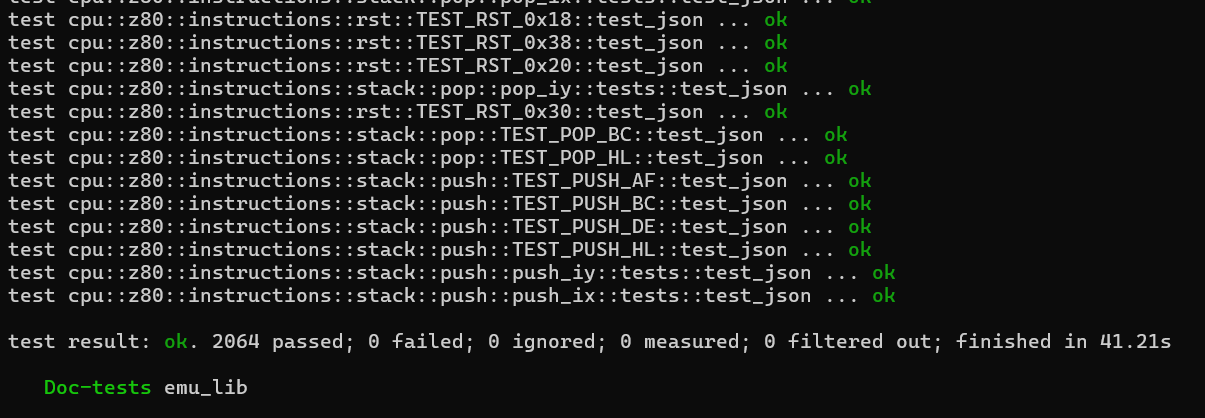
\includegraphics[width=0.8\textwidth]{images/testresults.png}
\caption{Rezultatele testelor automate}
\label{fig:testresults}
\end{figure}

Pentru fiecare instructiune au fost implementate 3 teste. 2 Teste fiind pentru testarea decodarii, iar unul pentru functionalitatea instructiunii.

\begin{itemize}
    \item {\code{as\_string\_and\_back}} Testul va transforma instructiunea in reprezentarea sa in string, apoi va incerca sa o decodeze inapoi in instructiune executabila. Pentru a trece testul instructiunea decodata trebuie sa fie instructiunea testata.
    \item {\code{as\_bytes\_and\_back}} Testul va transforma instructiunea in reprezentarea sa in cod masina, apoi va incerca sa o decodeze codul masina inapoi in instructiune executabila. Pentru a trece testul instructiunea decodata trebuie sa fie instructiunea testata.
    \item {\code{test\_json}} Testul va rula toate cele 1000 de cazuri specificate de SingleStepTests \cite {ref:singlesteptestsz80} pentru instructiunea testata. Pentru a trece testul toate cazurile trebuie sa fie finalizate cu succes, iar starea procesorului la final sa fie cea asteptata.
\end{itemize}

In timpul testarii instructiunilor au fost observate anomalii in special cu bitii 3 si 5 ai flag-ului F. Acestia nu sunt documentati in arhitectura Z80, dar totusi sunt folositi de unele instructiuni. Datorita faptului ca folosirea acestor biti nu este documentata, am decis sa ignoram verificarea lor in testele automate. Acest lucru a fost facut pentru a evita confuzii si pentru a nu introduce erori in emulator.

\begin{lstlisting}[language=Rust,caption={Ignorarea bitilor nedocumentati din testare},label={lst:testingignore35flags}]
    let mut result_flags = registers.gp.f;
    result_flags.set_bit3(false);
    result_flags.set_bit5(false);
    assert_eq!(result_flags, (state.f & 0b11010111).into());
\end{lstlisting}
\subsection{Interfata web}

Pentru a facilita utilizarea emulatorului, a fost implementata o interfata web folosind framework-ul Leptos. Leptos este un framework modern pentru dezvoltarea de aplicatii web in Rust, care permite crearea de interfete reactive si performante. Desi Leptos este inca in stadiul de dezvoltare, acesta ofera functionalitati avansate si o performanta ridicata. Comunitatea Leptos este in continua crestere, iar framework-ul este activ dezvoltat si intretinut.

De asemenea, pe langa leptos, Axum a fost folosit pentru a crea un server web care sa gestioneze cererile HTTP si sa serveasca interfata web. Axum este un framework web bazat pe Tokio, care ofera o abordare simpla si eficienta pentru dezvoltarea de aplicatii web in Rust.
Motivul principal din cauza caruia s-a ales Axum, a fost faptul ca are o compatibilitate foarte buna cu Leptos.

\subsubsection{Frontend}

Aplicatia este formata din 4 pagini:
\paragraph {Pagina principala} \cref {fig:homepage} Aceasta este pagina unde utiliztorul poate alege intre a se autentifica, inregistra sau a porni emulatorul
\begin{figure}[h!]
    \centering
    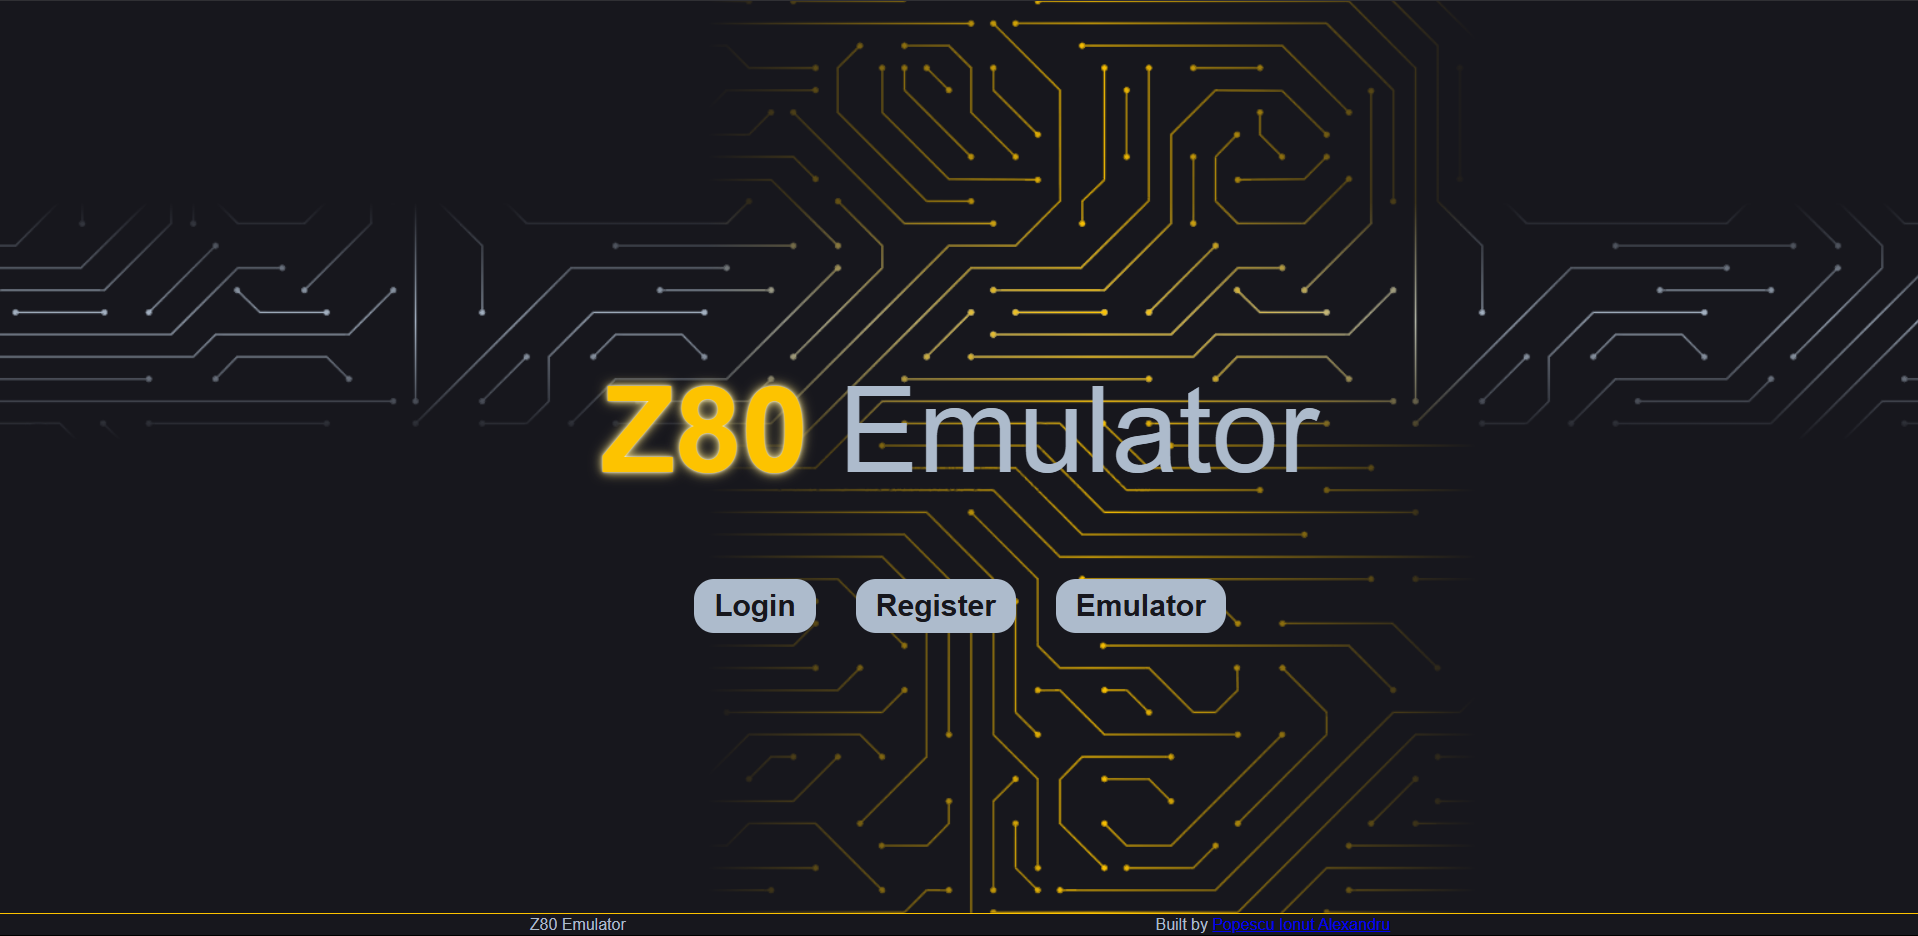
\includegraphics[width=0.8\textwidth]{images/homepage.png}
    \caption{Pagina principala a aplicatiei}
    \label{fig:homepage}
\end{figure}

\paragraph {Register} \cref {fig:registerpage} Pagina de inregistrare, unde utilizatorul trebuie sa isi numele de utilizator, emailul si parola pentru a se inregistra in aplicatie.
\begin{figure}[h!]
    \centering
    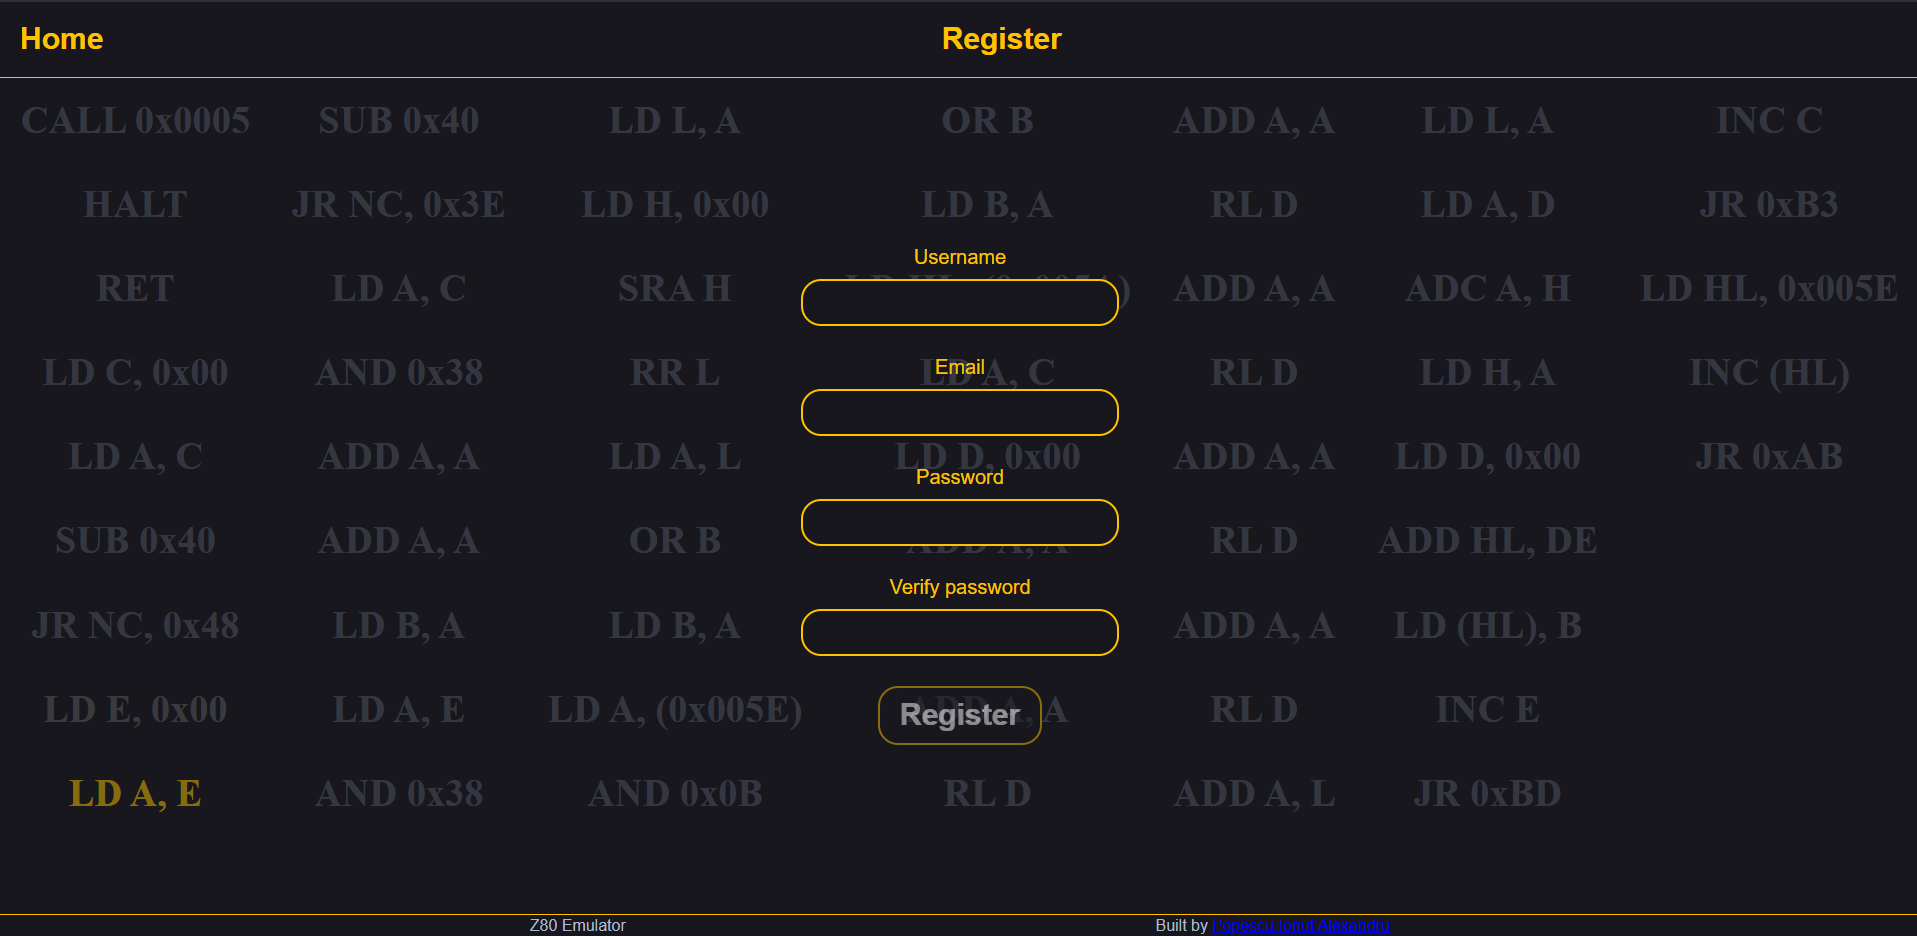
\includegraphics[width=0.8\textwidth]{images/registerpage.png}
    \caption{Pagina de inregistrare a aplicatiei}
    \label{fig:registerpage}
\end{figure}

\paragraph {Login} \cref {fig:loginpage} Pagina de autentificare, unde utilizatorul poate introduce numele de utilizator sau emailul si parola pentru a se autentifica in aplicatie.
\begin{figure}[h!]
    \centering
    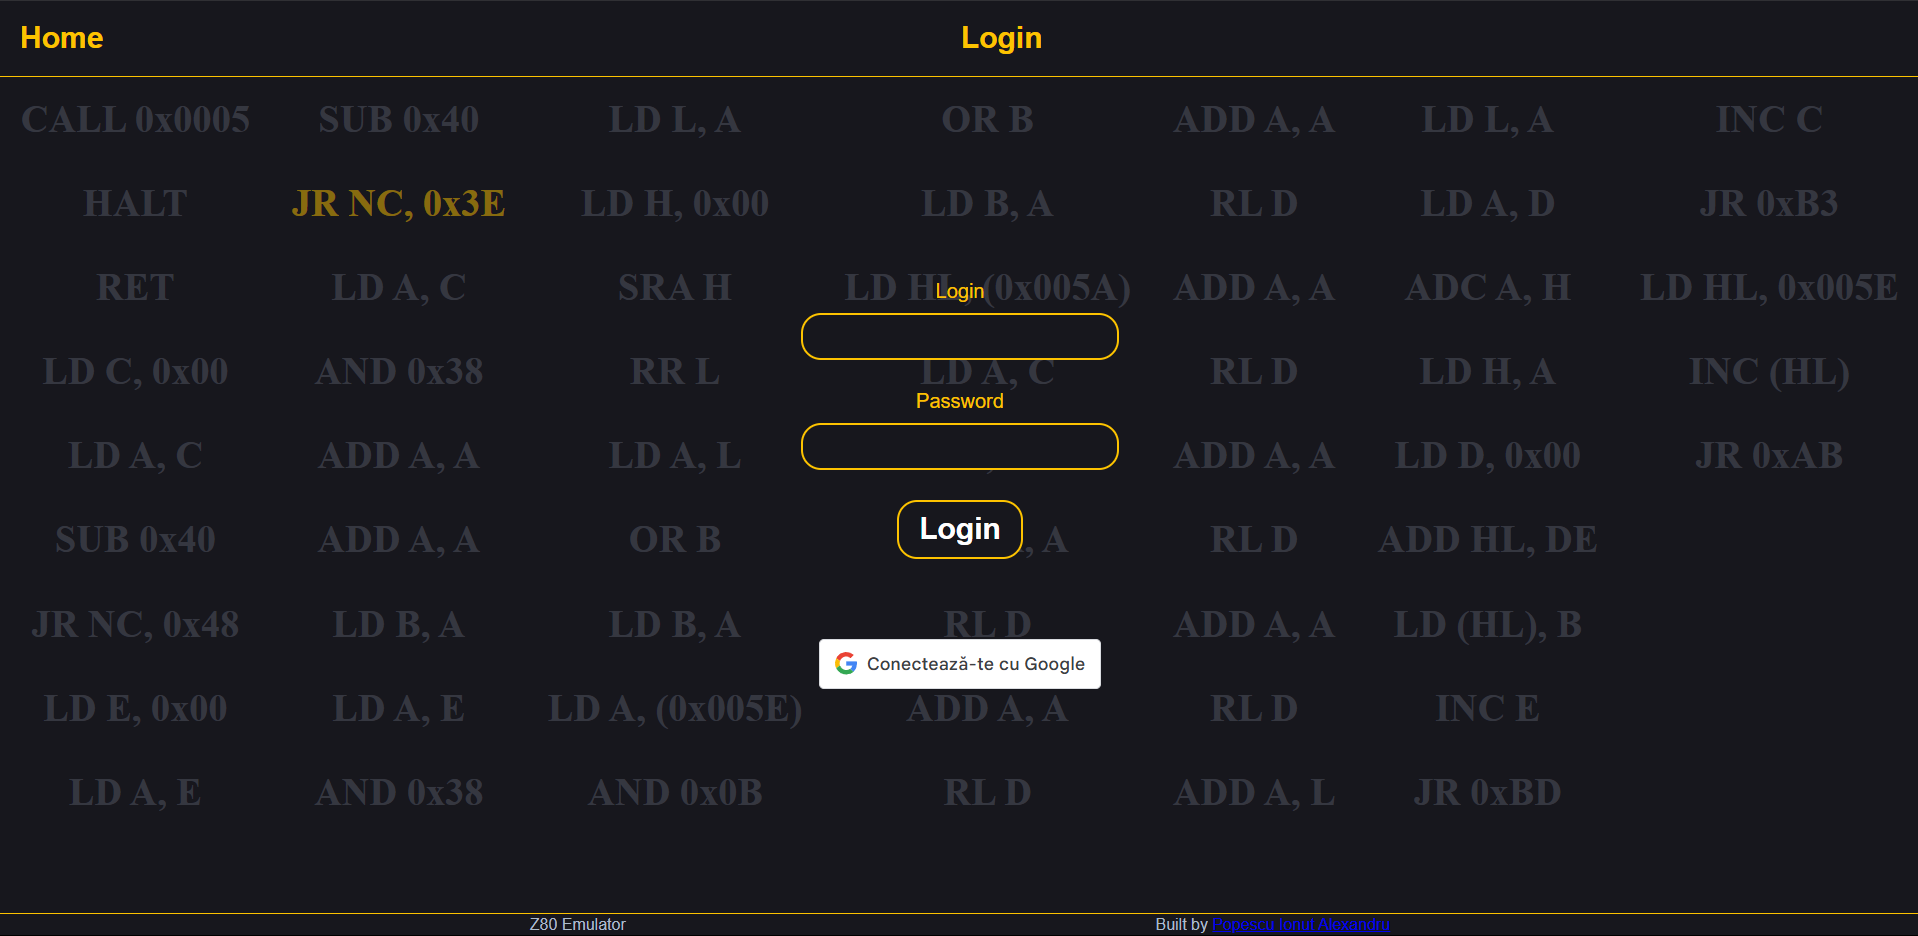
\includegraphics[width=0.8\textwidth]{images/loginpage.png}
    \caption{Pagina de autentificare a aplicatiei}
    \label{fig:loginpage}
\end{figure}

Elementul \code{<input>} pentru login este configurat sa accepte atat numele de utilizator cat si emailul, acest lucru fiind util pentru a permite utilizatorilor sa se autentifice cu oricare dintre cele doua. Acest element este reactiv si verifica in timp real existenta utilizatorului in baza de date prin a accesa APIul \code{/api/login\_exists}.\cref{lst:loginexistsapi}

 Cand utilizatorul modifica continutul campului, se va face o cerere catre server pentru a verifica daca utilizatorul exista. Daca utilizatorul nu exista, casuta va fi colorata in rosu, daca exista, aceasta va fi colorata in verde. Acest lucru ofera o feedback imediat utilizatorului si il ajuta sa evite erorile de autentificare.
Din motive de securitate, parola nu este verificata in timp real, aceasta fiind verificata doar la trimiterea formularului de autentificare. Daca aceasta functionalitate ar fi fost implementata si pentru campul de parola, acest lucru ar fi putut expune proiectul la atacuri de tip \emph{brute force}, deoarece un atacator ar fi putut incerca sa ghiceasca parola si sa primeasca feedback imediat daca aceasta este corecta sau nu. Limitarea numarului de incercari de accesare a acestui API pentru parola ar putea limita suprafata de atac, insa nu ar fi mitigat complet riscurile.

Cand butonul de login este apasat, se va face o cerere catre API-ul \code{/api/login} \cref{lst:loginapi}, care va verifica daca utilizatorul si parola sunt corecte. Daca acestea sunt corecte, utilizatorul va fi autentificat si redirectionat catre pagina emulatorului. Daca nu, se va afisa un mesaj de eroare.

Datorita faptului ca un numar mare de utilizatori au cont de Google, am implementat si posibilitatea de a se autentifica cu contul de Google. Acest lucru se face prin intermediul API-ului OAuth2, care permite utilizatorilor sa se autentifice cu contul lor de Google si sa acceseze aplicatia fara a fi nevoie sa creeze un cont separat.
Pentru implementarea acestei functionalitati, urmatoarele elemente au fost incluse in continutul \code{HTML} al paginii de autentificare:
\begin{lstlisting}[language=HTML,caption={Script necesar Google OAuth2},label={lst:googleauthscript}]
<Script src="https://accounts.google.com/gsi/client"
 defer="defer"
 async_="async"
/>
\end{lstlisting}
\begin{lstlisting}[language=HTML,caption={Butonul de autentificare cu Google},label={lst:googleauthbutton}]
<div id="g_id_onload"
    data-client_id=
    "652756675182-jij1vm0aiacih2mnhohc51tu32099n85.apps.googleusercontent.com"
    data-ux_mode="redirect"
    data-login_uri=format!("https://{public_url}/api/google_login_callback")
></div>
\end{lstlisting}


\paragraph {Emulator} \cref {fig:emulatorpage} Pagina in care utilizatorul poate interactiona cu emulatorul.
\begin{figure}[h!]
    \centering
    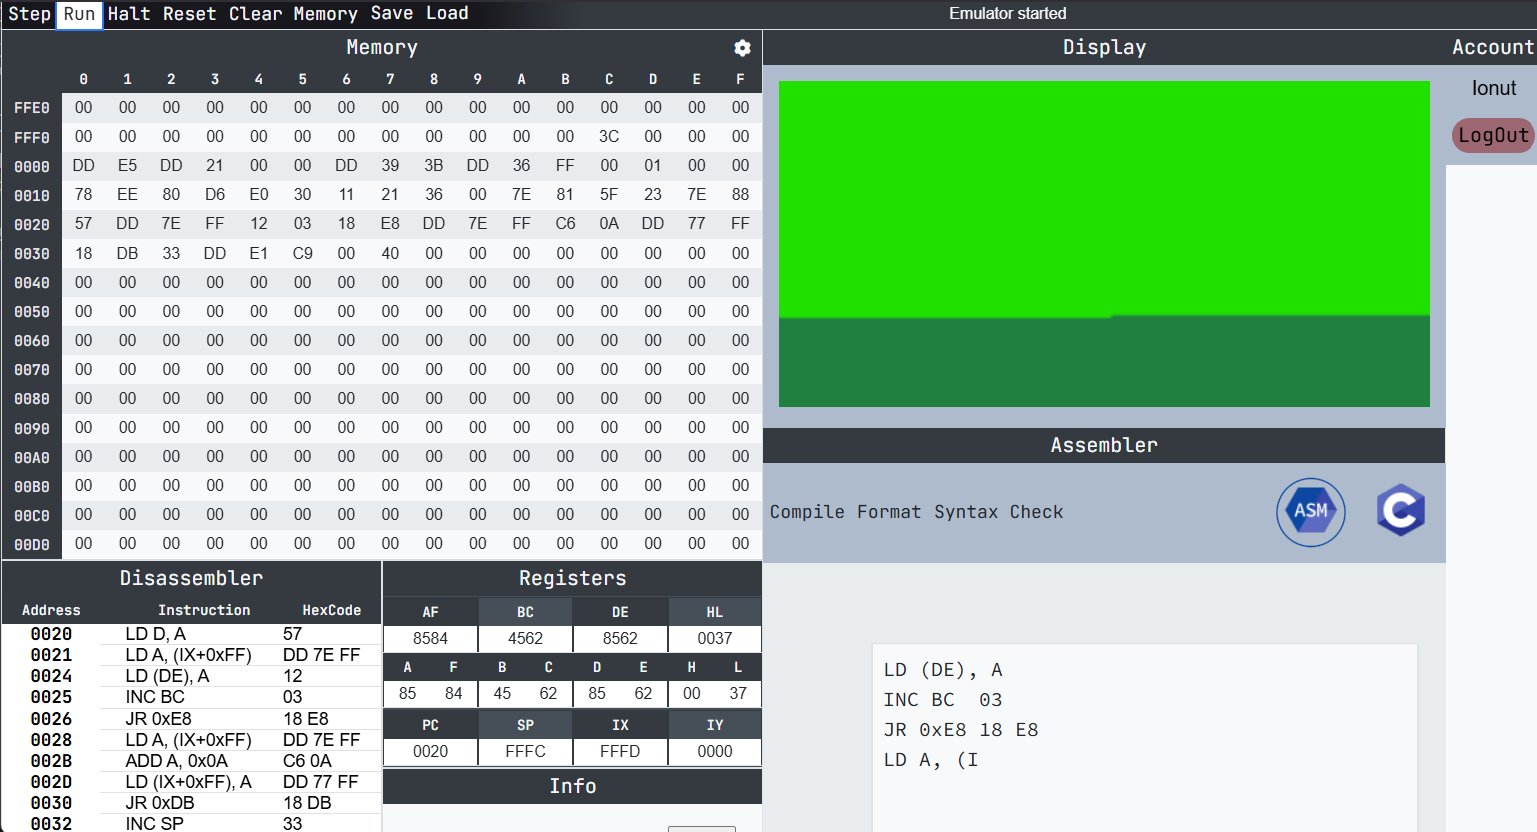
\includegraphics[width=0.8\textwidth]{images/emulatorpage.png}
    \caption{Pagina emulatorului}
    \label{fig:emulatorpage}
\end{figure}

Aceasta pagina este impartita in mai multe sectiuni:
\begin{itemize}
    \item {Status} - Aceasta va contine butoane pentru a controla emulatorul cat si ultimul mesaj de informare, avertisment sau eroare.
    \item {Memory} - Tabela ce contine si permite modificarea valorilor din memoria emulatorului.
    \item {Registrii} - Toti registrii emulatorului
    \item {Disassembler} - Contine instructiunile dezasamblate din memoria emulatorului.
    \item {Info} - Afiseaza numarul de ciclii si instructiuni executate de emulator.
    \item {Display} - Un ecran conectat la memoria emulatorului.
    \item {Assembler} - Editor si compiler de cod ASM si C.
    \item {Account} - Detalii cont
\end{itemize}

Pe partea de sus a paginii se poate vedea bara de comanda si status. Butoanele de comanda au urmatorul rol:
\begin{itemize}
    \item {\code{Step}} - Va trasa un singur pas in executia emulatorului, acest lucru va executa o singura instructiune si va actualiza registrii si statusul.
    \item {\code{Run}} - Va rula emulatorul pana cand acesta se opreste singur (Halt) sau pana cand utilizatorul apasa butonul din nou.
    \item {\code{Halt}} - Seteaza starea emulatorului la Halt, acest lucru va opri executia emulatorului. Acest status este setat de obicei doar de instructiunea Halt, si va restrictiona executarea instructiunilor pana este dezactivat de utilizator
    \item {\code{Reset}} - Reseteaza complet starea microprocesorului lasand memoria intacta. Doar registrii si numaratoarele de instructiuni si ciclii vor fi resetate.
    \item {\code{Clear Memory}} - Va reseta toata memoria emulatorului la valoarea de 0 in fiecare adresa. 
    \item {\code{Save}} - Va crea un fisier \code{emu\_memory.bin} cu datele din memoria emulatorului.
    \item {\code{Load}} - Va incarca un fisier ales de utilizator in memoria emulatorului.
\end{itemize}

Memoria emulatorului poate fi configurata astfel incat sa reprezinte datele in mai multe formate. Acestea pot fi: Hexadecimal, Decimal si ASCII. Utilizatorul poate alege formatul dorit din meniul dropdown din partea de sus-dreapta a tabelului de memorie. \cref{fig:memoryformat} arata cum se poate schimba formatul memoriei.


\begin{figure}[h!]
    \centering
    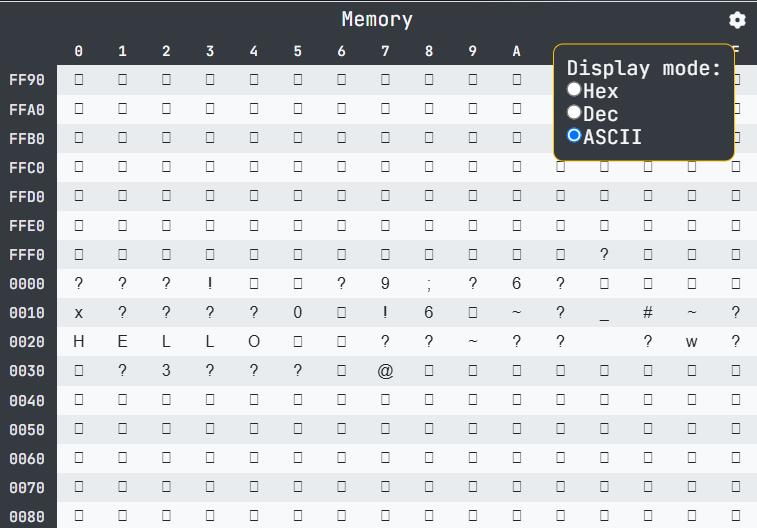
\includegraphics[width=0.8\textwidth]{images/memoryformat.png}
    \caption{Schimbarea formatului memoriei}
    \label{fig:memoryformat}
\end{figure}

\begin{minipage}{0.55\textwidth} % Text on the left
    In Disassembler \cref{fig:disassembler}, utilizatorul poate vedea instructiunile dezasamblate din memoria emulatorului. Acesta este configurat sa urmeze PC, instructiunile ce urmeaza a fi executate fiind mereu vizibile. Aici utilizatorul de asemenea are capabilitatea de a include breakpoint-uri. Introducerea de breakpoint-uri se face simplu, doar prin a da click in stanga instructiunii astfel incat sa apara un cerc rosu. Pentru stergerea unui breakpoint, utilizatorul trebuie sa dea click din nou pe cercul rosu, acesta va disparea si instructiunea nu va mai opri executia emulatorului. Capacitatea de a citii instructiunile impreuna cu cea de a oprii executia conditional la oricare dintre acestea este oferita cu scopul de a ajuta utilizatorul sa depaneze codul sursa al programului rulat in emulator. Acest lucru este util in special pentru programatorii care doresc sa inteleaga cum functioneaza codul lor sau pentru a gasi erori in acesta. Pentru o claritate mai ridicata, instructiunile sunt afisate in limbaj de asamblare Z80 dar si in cod masina.
\end{minipage}%
\hfill
\begin{minipage}{0.4\textwidth} % Image on the right
    \centering
    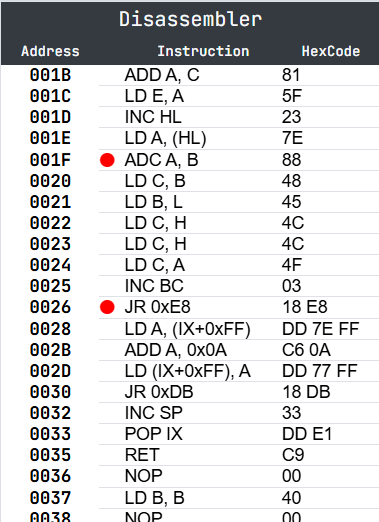
\includegraphics[width=\linewidth]{images/disassembler.png}
    \captionof{figure}{Disassembler} % needs \usepackage{caption}
    \label{fig:disassembler}
\end{minipage}

Ecranul emulatorului are o rezolutie de \code{192 X 128} pixeli, fiecare pixel fiind reprezentat de un byte in memorie. Fiecare byte reprezinta o culoare in format RGB in formatul \code{0xRRRGGGBB}, unde R, G si B sunt valorile de culoare rosu, verde si albastru. Acest lucru permite o paleta de 256 de culori diferite. Datorita rezolutiei sale si a faptului ca fiecare pixel este reprezentat de un byte, ecranul va ocupa 24KB in memorie. Memoria ecranului incepe de la adresa \code{0x4000} si se termina la adresa \code{0x9999}. Ecranul este actualizat la fiecare pas al emulatorului, astfel incat utilizatorul poate vedea imediat modificarile aduse de programul rulat in emulator.
Ecranul este creat prin a implementa \cref{lst:displaymemdevice} traitul \code{MemoryDevice} care permite displayului sa fie folosit ca un dispozitiv de memorie. Acest lucru permite ca ecranul sa fie tratat ca o parte a memoriei emulatorului, permitand astfel citirea si scrierea pixelilor direct in memorie. Aceasta implementare este utila pentru a permite programelor sa acceseze ecranul direct prin intermediul instructiunilor de citire si scriere in memorie



\begin{lstlisting}[language=Rust,caption={Implementare \code{MemoryDevice} display},label={lst:displaymemdevice}]
fn read_8(&self, addr: u16) -> Result<u8, MemoryReadError> {
    self.display.with(|data| {
        data.get(addr as usize)
            .map(|pixel| pixel.0)
            .map_err(|_| MemoryRWCommonError::OutOfBounds(addr).into())
    })
}

fn write_8(&mut self, addr: u16, value: u8) -> Result<(), MemoryWriteError> {
    let mut result: Result<(), MemoryWriteError> =
     Err(MemoryRWCommonError::OutOfBounds(addr).into());
    self.display.update(|data| {
        if let Ok(()) = data.set(addr as usize, U8Pixel::from(value)){
            result = Ok(());
        };
    });
    result
}
\end{lstlisting}

Datorita implementarii traitului \code{MemoryDevice}, in initializarea emulatorului \cref{lst:emulatorinitialization} memoria acestuia poate fi initializata cu ecranul \code{DisplayMemoryDevice}.
Primii 16KB din memorie vor fi ocupati de \code{RAM}, fiind urmati de ecranul emulatorului, iar restul de memorie va fi ocupat tot de \code{RAM}. Aceasta structura de memorie permite ca emulatorul sa aiba o memorie de 64KB, ceea ce este suficient pentru a rula majoritatea programelor scrise pentru \ac {Z80}. Aceasat functie de initializare a emulatorului va activa si inregistrarea modificarilor in memorie, astfel incat sa se poata urmari modificarile aduse de programul rulat in emulator. Acest lucru este util pentru a putea depana codul sursa al programului sau pentru a putea vedea cum functioneaza acesta. La fiecare pas al emulatorului, tabela \code{Memory} va afisa cu galben doar valorile care au fost schimbate.
\begin{lstlisting}[language=Rust,caption={Initializarea emulatorului},label={lst:emulatorinitialization}]
fn build_z80_emu(display: DisplayMemoryDevice) -> Emulator<Z80> {
    use emu_lib::memory;
    use emu_lib::memory::MemoryDevice;
    let mut memory = memory::Memory::new();
    let initial_ram_size = 0x4000;
    let initial_ram = memory::memdevices::RAM::new(initial_ram_size);
    let post_ram = memory::memdevices::RAM::new(
        0x10000 - initial_ram_size - display.size()
    );
    memory.add_device(Box::new(initial_ram));
    memory.add_device(Box::new(display));
    memory.add_device(Box::new(post_ram));
    let mut emu = Emulator::<Z80>::new_w_mem(memory);
    emu.memory.record_changes(true);
    emu
}
\end{lstlisting}

Pentru ecranul afisarea datelor de pe ecranul emulatorlui un element de tip \code{<canvas>} este folosit, acesta va fi actualizat la fiecare pas al emulatorului. In acest fel, utilizatorul poate vedea imediat modificarile aduse de programul rulat in emulator. Datele de pe ecran sunt luate direct din structura \code {DisplayData}, aceasta implementand urmatoarele metode \cref {lst:displaydatamethods} pentru setarea si citirea unui pixel la coordonatele \code{(x, y)}:
\begin{lstlisting}[language=Rust,caption={Metodele de setare si citire a pixelilor},label={lst:displaydatamethods}]
pub fn set_pixel(&mut self, x: usize, y: usize, color: U8Pixel) ->
    Result<(), &'static str> {
        let index = self.get_index(x, y)?;
        self.set(index, color)
    }

    pub fn get_pixel(&self, x: usize, y: usize) -> Result<U8Pixel, &'static str> {
        let index = self.get_index(x, y)?;
        self.get(index)
    }
\end{lstlisting}

Functia \code{set\_pixel} va primi pe langa coordonatele pixelului si culoarea acestuia. Culoarea fiind reprezentata de un \code{U8Pixel}, un tip de date care permite convertirea usoara in sau din formatul RGB. \cref{lst:u8pixel}

\begin{lstlisting}[language=Rust,caption={Tipul de date U8Pixel},label={lst:u8pixel}]
#[derive(Clone,Copy, Debug, PartialEq, Eq, Hash)]
pub struct U8Pixel(pub u8);

impl U8Pixel {
    pub fn from_rgb(r: u8, g: u8, b: u8) -> Self {
        // r 3 bits, g 3 bits, b 2 bits
        let pixel_value = (r & 0b11100000)
            | ((g & 0b11100000) >> 3)
            | (b & 0b11000000 >> 6);
        U8Pixel(pixel_value)
    }

    pub fn to_rgb(&self) -> (u8, u8, u8) {
        //topmost bits
        let r = self.0 & 0b11100000; // 3 bits for red
        let g = (self.0 & 0b00011100) << 3; // 3 bits for green
        let b = (self.0 & 0b00000011) << 5; // 2 bits for blue
        (r, g, b)
    }
}
impl From<u8> for U8Pixel {
    fn from(value: u8) -> Self {
        U8Pixel(value)
    }
}

impl From<U8Pixel> for u8 {
    fn from(value: U8Pixel) -> Self {
        value.0
    }
}
\end{lstlisting}

Un lucru important este ca transformarea din RGB in U8Pixel este \code{lossy}, adica se pierde o parte din informatii. Acest lucru se datoreaza faptului ca U8Pixel foloseste doar 8 biti pentru a reprezenta culoarea, in timp ce RGB foloseste 24 de biti. Acest lucru inseamna ca nu toate culorile RGB pot fi reprezentate in U8Pixel.

Partea de \code{Assembler} \cref{fig:assembler} este un editor de cod sursa care permite utilizatorului sa scrie cod in limbajul de asamblare Z80 sau in limbajul C. Acesta este un editor simplu de text care ofera functionalitat de baza precum asamblare/compilare, formatare si verificare a sintaxei programului.

\begin{figure}[H]
    \centering
    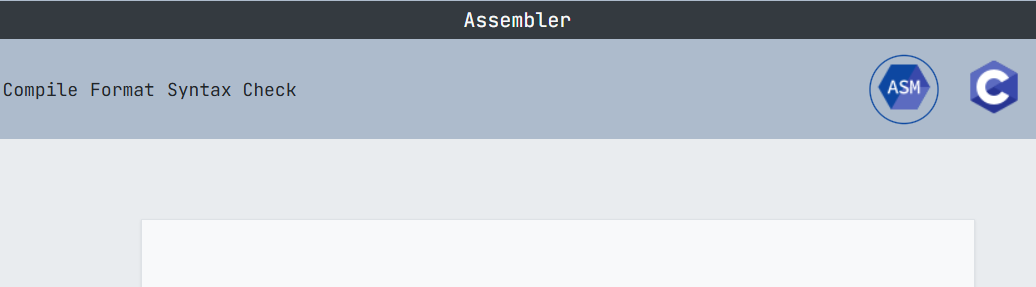
\includegraphics[width=0.8\textwidth]{images/assembler.png}
    \caption{Editorul de cod sursa al emulatorului}
    \label{fig:assembler}
\end{figure}

In partea de sus a editorului se pot vedea butoanele de asamblare/compilare, formatare si verificare a sintaxei. Butonul de asamblare/compilare va incerca sa transforme codul sursa in cod masina, iar daca acest lucru reuseste, il va copia in memoria emulatorului. In cazul in care asamblarea/compilarea esueaza, utilizatorul va primi un mesaj de eroare cu detalii despre eroarea intalnita. Butonul de formatare va incerca sa formateze codul sursa pentru a fi mai usor de citit, iar butonul de verificare a sintaxei va verifica daca codul sursa este valid si nu contine erori de sintaxa.

In partea din dreapta a editorului se va face selectia dintre limbajul de asamblare Z80 si limbajul C. In cazul in care utilizatorul alege limbajul C, editorul va incerca sa compileze codul sursa folosind compilatorul \code{gcc}. Daca compilarea reuseste, codul masina rezultat va fi copiat in memoria emulatorului. In cazul in care compilarea esueaza, utilizatorul va primi un mesaj de eroare cu detalii despre eroarea intalnita.

In partea de jos a editorului se poate vedea un \code{<textbox>} in care utilizatorul poate introduce codul in limbajul de programare selectat. Fiecare limbaj de programare va avea propriul sa buffer, astfel incat atunci cand utilizatorul schimba limbajul de programare, codul sursa va fi salvat in bufferul corespunzator. Acest lucru permite utilizatorului sa schimbe intre limbajele de programare fara a pierde codul sursa scris.

\begin{minipage}[c]{0.55\textwidth} % Text on the left
    Sectiunea de \code{Registers} \cref{fig:registerssection} afiseaza toti registrii procesorului Z80, inclusiv registrii generali, registrii de indexare si registrul de stare. Acestia sunt afisati in format hexadecimal, iar utilizatorul poate modifica valorile acestora direct din interfata web. Aceasta functionalitate este utila pentru a putea depana codul sursa al programului rulat in emulator sau pentru a putea modifica starea procesorului in timpul executiei.
\end{minipage}%
\hfill
\begin{minipage}[c]{0.4\textwidth} % Image on the right
    \centering
    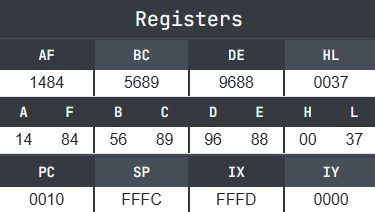
\includegraphics[width=0.8\textwidth]{images/registerssection.png}
    \captionof{figure}{Sectiunea de registrii a emulatorului}
    \label{fig:registerssection}
\end{minipage}

\subsubsection{Backend}

\paragraph{Middleware} este un set de functii care sunt apelate inainte de a ajunge la handlerul API. Acestea sunt folosite pentru a face diverse verificari si pentru a seta contextul pentru handlerul API. De exemplu, middleware-ul \code{auth\_middleware} \cref{lst:authmiddleware} verifica daca utilizatorul este autentificat si seteaza utilizatorul in contextul API-ului. Acest lucru permite handlerelor API sa acceseze informatiile despre utilizatorul autentificat fara a fi nevoie sa le primeasca ca parametru.

\begin{lstlisting}[language=Rust,caption={Middleware pentru autentificare},label={lst:authmiddleware}]
pub async fn auth_middleware(
    State(app_state): State<AppState>,
    mut req: Request,
    next: Next,
) -> Result<Response, StatusCode> {
    let pool = app_state.pool;
    if let Some(session_token) =
     cookie::server::get(&CookieKey::Session, &req.headers()) {
        if let Ok(session) =
         Session::get_by_token(&session_token, &pool) {
            if !session.is_expired() {
                if let Ok(user) =
                 User::get_by_id(session.user_id, &pool) {
                    let user_data: UserData = user.into();
                    req.extensions_mut().insert(user_data);
                }
            }
        }
    }
    Ok(next.run(req).await)
}
\end{lstlisting}

Motivul din caza caruia s-a ales sa se foloseasca middleware-uri este faptul ca acestea ca odata ce o extensie este adaugata in contextul API-ului, aceasta va putea fi accesta in \code{server methods} din framework-ul Leptos. Acest lucru permite ca informatiile despre utilizatorul autentificat sa fie accesibile in toate handlerile API, fara a fi nevoie sa le primim ca parametru. Acest lucru este util pentru a putea verifica daca utilizatorul are permisiunea de a accesa anumite resurse sau de a efectua anumite actiuni. In cadrul emulatorul singurele actiuni care sunt limitate doar pentru utilizatorii autentificati sunt compilarea, formatarea si verificarea sintaxei programelor din limbaaul C. Acest lucru este facut pentru a limita accessul la resursele serverului si pentru a preveni abuzurile. In cazul in care utilizatorul nu este autentificat, acesta va primi un mesaj de eroare si nu va putea accesa compilarea programelor din limbajul C.

\paragraph{API\-uri de autentificare} sunt implementare folosing server methods din framework-ul Leptos. Acestea sunt folosite pentru a permite utilizatorilor sa se autentifice, sa se inregistreze si sa se deconecteze din aplicatie. Aceste API-uri sunt implementate in modulul \code{auth} si sunt accesibile prin intermediul URL-urilor \code{/api/login}, \code{/api/register} si \code{/api/logout} ...etc. Acestea sunt implementate folosind server methods din framework-ul Leptos, care permite crearea de API-uri RESTful in mod simplu si eficient.

\begin{lstlisting}[language=Rust,caption={API pentru verificarea existentei utilizatorului},label={lst:loginexistsapi}]
 #[server(LoginExistsApi, endpoint = "/login_exists")]
 pub async fn login_exists(login: String)
  -> Result<bool, ServerFnError> {
     use server_imports::*;
     let state = expect_context::<AppState>();
     let pool = &state.pool;
     match User::get_by_login(&login, &pool) {
         Ok(Some(_)) => Ok(true),
         Ok(None) => Ok(false),
         Err(err) => Err(ServerFnError::Response(format!(
             "Failed to check login: {}",
             err
         ))),
     }
 }
 \end{lstlisting}
 Functia \code{login\_exists} \cref{lst:loginexistsapi} ruleaza doar pe server si verifica daca utilizatorul exista in baza de date. Daca utilizatorul exista, va returna \code{true}, altfel va returna \code{false}.


 Pentru autentificare se va folosi functia \code{login} \cref{lst:loginapi}, aceasta va incerca sa obtina utilizatorul din baza de date folosind numele de utilizator sau emailul si parola. Daca utilizatorul este gasit si parola este corecta, se va crea o sesiune pentru utilizator si se va seta un cookie de sesiune. Daca utilizatorul nu este gasit sau parola este incorecta, se va returna o eroare.
 \begin{lstlisting}[language=Rust,caption={API pentru autentificare},label={lst:loginapi}]
 #[server(LoginApi, endpoint = "/login")]
 pub async fn login(login: String, password: String) -> Result<(), ServerFnError> {
     use server_imports::*;
     let response = expect_context::<ResponseOptions>();
     let state = expect_context::<AppState>();
     // let state: Extension<AppState> = extract().await?;
     let pool = &state.pool;
     let user_login = UserLogin::new(login, password);
     match user_login.get_user(&pool) {
         Ok(user) => {
             if let Ok(session) =
              user.authenticate(&pool, AUTH_TIMEOUT)
             {
                 cookie::server::set(&CookieKey::Session,
                  &session.token, AUTH_TIMEOUT, &response)?;
                 Ok(())
             }else {
                 Err(ServerFnError::ServerError(
                 "Failed to authenticate user".to_string()))
             }
         }
         Err(e) => {
             cookie::server::remove(&CookieKey::Session, &response)?;
             response.set_status(StatusCode::UNAUTHORIZED);
             let msg = format!("Failed to login user: {}", e);
             Err(ServerFnError::Response(msg))
         }
     }
 }
 \end{lstlisting}

 Pentru autentificarea cu Google, se va folosi API-ul \code{/api/google\_login\_callback} \cref{lst:googleloginapi}. Dupa ce utilizatorul se autentifica cu Google, acesta va fi redirectionat catre acest API trimitand urmatorii parametri:
\begin{itemize}
    \item \code{clientId} - ID-ul clientului Google, create in consola Google Cloud pentru a putea folosi API-ul Google OAuth2
    \item \code{client\_id} - ID-ul clientului Google (acesta este un parametru redundant, dar este necesar pentru a fi compatibil cu API-ul Google)
    \item \code{select\_by} - metoda de selectare a utilizatorului (de obicei este \code{sub})
    \item \code{g\_csrf\_token} - tokenul CSRF generat de Google
    \item \code{credential} - credentialul primit de la Google
\end{itemize}

Dupa ce API-ul primeste aceste date, acesta va folosi libraria \code{google\_oauth} pentru a valida tokenul primit de la Google. Daca tokenul este valid, API-ul va incerca sa obtina utilizatorul din baza de date folosind ID-ul utilizatorului Google. Daca utilizatorul exista, acesta va fi autentificat si se va crea o sesiune pentru acesta. Daca utilizatorul nu exista, acesta va fi creat in baza de date folosind numele si emailul primit de la Google. In cazul in care crearea utilizatorului esueaza, se va returna o eroare.
Cand un cont isi creaza un cont prin Google, acesta va primi o parola generata aleatoriu. Aceast lucru a fost facut deoarece campul de parola este obligatoriu in baza de date. Utilizatorul nu va primi aceasta parola, deoarece autentificarea se va face doar prin Google.
In baza de date, utilizatorul va avea un camp \code{oauth\_google} care va contine ID-ul utilizatorului Google. Acest camp va fi folosit pentru a identifica utilizatorul in cazul in care acesta se autentifica din nou cu Google.
\begin{lstlisting}[language=Rust,caption={API pentru autentificarea cu Google},label={lst:googleloginapi}]
#[allow(non_snake_case)]
#[server(GoogleLoginCallbackApi, endpoint = "/google_login_callback")]
pub async fn google_login_callback(
    clientId: String,
    client_id: String,
    select_by: String,
    g_csrf_token: String,
    credential: String,
) -> Result<(), ServerFnError> {
    use server_imports::*;
    let oauth_client = google_oauth::AsyncClient::new(clientId);
    let state = expect_context::<AppState>();
    let payload = oauth_client
        .validate_id_token(credential)
        .await
        .expect("Could not validate payload");
    if let Some(user) = get_google_user(&payload.sub) {
        user_auth(user, AUTH_TIMEOUT).await
    } else {
        //create random password
        let random_password: String = (0..16)
            .map(|_| rand::random::<char>()).collect();
        if let (Some(name),Some(email)) =
            (payload.name,payload.email) {
            let name = name.split(" ").next();
            let name = match name {
                Some(n) => n.to_string(),
                None => {
                    return Err(ServerFnError::Response(
                        "Could not get name for Google Auth registration"
                            .to_string(),
                    ))
                }
            };
            let new_user = NewUser::new(
                name,
                email.clone(),
                random_password.clone(),
                Some(payload.sub.clone()),
                None,
            );
            if let Ok(user) = new_user {
                if let Ok(user) = User::add_user(user, &state.pool) {
                    user_auth(user, time::Duration::seconds(60 * 60 * 24)).await?;
                    Ok(())
                    //...
\end{lstlisting}

In functie de rezultatul autentificarii, utilizatorul va fi redirectionat catre pagina emulatorului sau va primi un mesaj de eroare.

Pentru inregistrare, se va folosi API-ul \code{/api/register} \cref{lst:registerapi}. Acesta va primi numele, emailul si parola utilizatorului si va incerca sa creeze un nou utilizator in baza de date. Daca utilizatorul este creat cu succes, functia va returna un rezultat de tip \code{Ok(())}. In cazul in care crearea utilizatorului esueaza, se va returna o eroare cu un mesaj corespunzator, fie ca este o eroare de validare a datelor, fie ca este o eroare de baza de date. In ambele cazuri, statusul HTTP va fi setat la \code{BAD\_REQUEST (400)} pentru a indica faptul ca cererea nu a fost procesata cu succes.

\begin{lstlisting}[language=Rust,caption={API pentru inregistrare},label={lst:registerapi}]
#[server(RegisterApi, endpoint = "/register")]
pub async fn register(
    username: String,
    email: String,
    password: String,
) -> Result<(), ServerFnError> {
    use server_imports::*;
    let response = expect_context::<ResponseOptions>();
    let state = expect_context::<AppState>();
    let pool = &state.pool;
    match NewUser::new(username, email, password, None, None) {
        Ok(user) => match User::add_user(user, &pool) {
            Ok(_) => Ok(()),
            Err(e) => {
                response.set_status(StatusCode::BAD_REQUEST);
                let msg = format!("Failed to register user: {}", e);
                Err(ServerFnError::Response(msg))
            }
        },
        Err(e) => {
            response.set_status(StatusCode::BAD_REQUEST);
            let msg = format!("Failed to register user: {}", e);
            Err(ServerFnError::Response(msg))
        }
    }
}
\end{lstlisting}

Pentru returnarea datelor despre utilizatorul autentificat, se va folosi API-ul \code{/api/userdata} \cref{lst:userdataapi}. Acesta va incerca sa extraga datele despre utilizatorul autentificat din contextul API-ului, date aduse de middleware-ul de autentificare. Daca utilizatorul este autentificat, API-ul va returna datele despre utilizator, altfel va returna o eroare de tip \code{Unauthenticated}. Acest API este folosit pentru a obtine informatii despre utilizatorul autentificat, cum ar fi numele, emailul si ID-ul utilizatorului. Aceste informatii sunt folosite in interfata web pentru a afisa detalii despre utilizatorul autentificat cum ar fi numele pe pagina emulatorului \cref{fig:emulatorpage}.

\begin{lstlisting}[language=Rust,caption={API pentru obtinerea datelor despre utilizatorul autentificat},label={lst:userdataapi}]
#[server(GetUserData, endpoint = "/userdata")]
pub async fn userdata() -> Result<UserData, UserDataError> {
    use server_imports::*;
    let userdata: Result<Extension<UserData>, _> = extract().await;
    if let Ok(userdata) = userdata {
        Ok(userdata.0.clone())
    } else {
        Err(UserDataError::Unauthenticated)
    }
}
\end{lstlisting}

\paragraph{API\-ul compiler C} este implementat in fisierul \code{compiler.rs} si este folosit pentru a comunica cu serviciul de compilare.

Deoarece compilerul functioneaza pe alta masina, pentru a fiecare endpoint pe care il vrem acesibil 2 functii vor fi implementate. Una va fi scrisa in python si va functiona ca wrapper ce expune un API web compilatorului, iar cealalta va fi scrisa in Rust si va fi folosita pentru a face cereri catre API-ul web al compilatorului. Acest lucru permite ca frontend-ul sa poate comunica cu compilatorul fara a fi nevoie sa cunoasca detalii despre implementarea acestuia.

API-ul Python care ruleaza in containerul cu compilatorul C este implementat in fisierul \code{api.py} \cref{lst:compilerapi}. Acesta expune urmatoarele endpoint-uri:
\begin{itemize}
    \item \code{/compile} - pentru a compila codul sursa in limbajul C
    \item \code{/format} - pentru a formata codul sursa in limbajul C
    \item \code{/check\_syntax} - pentru a verifica sintaxa codului sursa in limbajul C
\end{itemize}

\begin{lstlisting}[language=Python,caption={API-ul Python pentru compilatorul C},label={lst:compilerapi}]
from fastapi import FastAPI
from pydantic import BaseModel
from pydantic.dataclasses import dataclass
from tempfile import TemporaryDirectory, NamedTemporaryFile
import base64
import subprocess
#...
def compile_str(b64data_in: str) -> CompileData:
    data_in = base64.b64decode(b64data_in).decode("utf-8")
    with TemporaryDirectory() as temp_dir:
        with open(f"{temp_dir}/{FILENAME}.c", "w") as f:
            f.write(data_in)
        command = ["zcc", "+z80", "-vn", "-O3", "-startup=31",
                   "-o", f"{FILENAME}.rom", "-create-app",
                   f"{FILENAME}.c", "-compiler=sdcc",
                   "-zorg=0x0", "-lm"]
        result = subprocess.run(
            command,
            cwd=temp_dir,
            stdout=subprocess.PIPE,
            stderr=subprocess.PIPE,
        )
        data: bytes = b""
        try:
            with open(f"{temp_dir}/{FILENAME}.rom", "rb") as f:
                data = f.read()
        except  FileNotFoundError:
            data = b""
        return CompileData(rc=result.returncode,
                           b64stdout=base64.b64encode(result.stdout),
                           b64stderr=base64.b64encode(result.stderr),
                           b64data=base64.b64encode(data))

def format_str(b64data_in: str) -> FormatData:
    data_in = base64.b64decode(b64data_in).decode("utf-8")
    with NamedTemporaryFile(mode="w+", suffix=".c") as f:
        f.write(data_in)
        f.flush()
        command = [
            "astyle",
            "--style=attach",
            "--indent=spaces=4",
            "--suffix=none",
            f.name
        ]
        result = subprocess.run(
            command,
            stdout=subprocess.DEVNULL,
            stderr=subprocess.DEVNULL,
        )
        data = b""
        if result.returncode == 0:
            f.seek(0)
            data = f.read().encode("utf-8")
        return FormatData(b64data=base64.b64encode(data))

def syntax_check(b64data_in: str) -> SyntaxCheckData:
    data_in = base64.b64decode(b64data_in).decode("utf-8")
    with NamedTemporaryFile(mode="w+", suffix=".c") as f:
        f.write(data_in)
        f.flush()
        command = ["gcc", "-fsyntax-only", f.name]
        result = subprocess.run(
            command,
            stdout=subprocess.DEVNULL,
            stderr=subprocess.PIPE,
        )
        return SyntaxCheckData(rc=result.returncode,
                               b64stderr=base64.b64encode(result.stderr))

class RequestDataModel(BaseModel):
    b64data: str

@app.post("/compile")
def compile_data_endpoint(item: RequestDataModel):
    return compile_str(item.b64data)

@app.post("/format")
def format_data_endpoint(item: RequestDataModel):
    return format_str(item.b64data)

@app.post("/syntax_check")
def syntax_check_endpoint(item: RequestDataModel):
    return syntax_check(item.b64data)
\end{lstlisting}

Pentru a serializa datele de intrare si iesire ale API-ului, se folosesc clasele \code{CompileData}, \code{FormatData} si \code{SyntaxCheckData}. Acestea sunt definite in fisierul \code{api.py} si sunt folosite pentru a serializa datele de intrare si iesire ale API-ului. Aceste clase sunt folosite pentru a serializa datele in format JSON, astfel incat sa poata fi trimise si primite prin intermediul API-ului.
Deoarece JSON nu este perfect pentru a serializa datele binare, datele binare sunt codificate in \code{base64} inainte de a fi trimise.

Deoarece pentru compilarea programelor se doreste o eficienta cat mai ridicata, compilatorul C a fost configurat sa fie cat mai minim. Parametrul \code{--startup=31} din comanda de compilare se asigura ca doar codul scris de utilizator va fi compilat, acest lucru inseamna ca nici macar \ac{CRT} nu va fi inclus in codul compilat. Acest lucru este util pentru a reduce dimensiunea codului compilat si pentru a permite utilizatorului sa controleze complet codul rulat in emulator. De asemenea, acest lucru permite ca emulatorul sa ruleze mai rapid, deoarece nu va fi nevoie sa se execute cod suplimentar pentru a initializa mediul de executie. Eventual acest comportament poate fi dezvoltat in continuare incat utilizatorul sa poate configura singur parametrii de compilare, dar acest lucru nu a fost implementat inca.

\ac {CRT} contine functia \code{\_start} care este punctul de intrare al programului C. Aceasta functie este responsabila pentru initializarea mediului de executie si pentru apelarea functiei \code{main}. In cazul in care \ac {CRT} nu este inclus in codul compilat, utilizatorul va trebui sa scrie singur functia \code{\_start} si sa apeleze functia \code{main} manual, numele functiei \code{\_start} poate fi schimbat, insa este important faptul ca orice nume ar avea, prima functie din program va fi apelata prima. In \cref{lst:nocrtcode} este prezentat un exemplu de cod C care nu include \ac {CRT} si care va rula in emulatorul nostru. Acest cod va scrie valoarea \code{0xFF} in locatia \code{0x50} de memorie si va termina executia. Acest lucru este util pentru a putea testa daca emulatorul functioneaza corect si daca poate rula cod C fara a include \ac{CRT}.
\begin{lstlisting}[language=C,caption={Cod C fara CRT},label={lst:nocrtcode}]
#include <intrinsic.h>
void _start() {
    main();
}
void set_val(){
    *(char*)0x50=0x50;
}
int main(){
    set_val();
    intrinsic_halt();
}
\end{lstlisting}
Functia \code{intrinsic\_halt} este o functie speciala care va seta starea procesorului in starea de \code{halt}, adica va opri executia programului. Aceasta functie este utila pentru a putea termina executia programului fara a fi nevoie sa se scrie cod suplimentar pentru a termina programul. In cazul in care aceasta functie nu este apelata, emulatorul va continua sa ruleze si va astepta ca utilizatorul sa apese butonul de oprire al emulatorului. Diferite functii pentru apel direct la instructiuni Z80 sunt implementate de libraria \code{intrinsic.h}.

Pentru formatarea codului sursa in limbajul C, enpointul \code{/format} va primi codul sursa in format \code{base64} si va returna codul sursa formatat tot in format \code{base64}. Acest lucru permite utilizatorului sa poata formata codul sursa fara a fi nevoie sa o faca manual. Endpointul va folosi modulul python \code{astyle} pentru a formata codul sursa. Acest modul este folosit pentru a formata codul sursa in conformitate cu standardele de codare C. Acesta nu returneaza un cod de eroare, ci doar codul sursa formatat. In cazul in care formatarea esueaza, fisierul returnat va fi acelasi cu cel primit ca input.

Pentru verificarea sintaxei codului sursa in limbajul C, endpointul \code{/syntax\_check} va primi codul sursa in format \code{base64} si va returna un cod de eroare si un mesaj de eroare in cazul in care sintaxa este incorecta. In cazul in care sintaxa este corecta, endpointul va returna un cod de succes (0) si fara mesaj de eroare. Acest lucru permite utilizatorului sa poata verifica sintaxa codului sursa fara a fi nevoie sa o faca manual. Endpointul va folosi compilatorul \code{gcc} pentru a verifica sintaxa codului sursa.

Pentru fiecare dintre API-urile de mai sus, exista o pereche de functii in Rust care sunt folosite pentru a face cereri catre API-ul Python. Aceste functii sunt implementate in fisierul \code{ccompiler.rs} sunt bazate pe libraria \code{Axum} si \code{Leptos}. In \cref{lst:compilerustapi} este prezentata functia \code{c\_compile} care este folosita pentru a compila codul sursa in limbajul C. Aceasta functie va primi de la browser codul sursa in format \code{String}, il va codifica in format \code{base64} si il va trimite catre API-ul Python. Daca compilarea reuseste, functia va returna un obiect de tip \code{CompileData} care contine codul de iesire al compilatorului, stdout-ul si stderr-ul. Daca compilarea esueaza, functia va returna o eroare de tip \code{CompilerError}. In cazul in care utilizatorul nu este autentificat, functia va returna o eroare de tip \code{Unauthorized} si va seta statusul HTTP la \code{UNAUTHORIZED (401)}.

\begin{lstlisting}[language=Rust,caption={API Rust pentru compilarea codului C},label={lst:compilerustapi}]
#[server(CCompile, endpoint = "/ccompile")]
pub async fn c_compile(code: String) -> Result<CompileData, CompilerError> {
    use crate::db::models::user::UserData;
    use server_imports::*;
    //encode code in b64
    let data = RequestBody::new(code);
    let state = expect_context::<AppState>();
    let response = expect_context::<ResponseOptions>();
    let userdata: Result<Extension<UserData>, _> = extract().await;
    match userdata {
        Ok(_) => {
            let reqwest_client = &state.reqwest_client;
            let response = reqwest_client
                .post(format!("http://{}/compile",*COMPILER_HOST))
                .header(
                    "Content-Length",
                    serde_json::to_string(&data).unwrap().len(),
                )
                .json(&data)
                .send()
                .await
                .map_err(|e| CompilerError::RequestError(e.to_string()))?
                .json::<EncCompileData>()
                .await
                .map_err(|e| CompilerError::RequestError(e.to_string()))?;
            response.decode()
        }
        Err(_) => {
            response.set_status(StatusCode::UNAUTHORIZED);
            Err(CompilerError::Unauthorized)
        }
    }
}
\end{lstlisting}

Pentru formatarea codului sursa in limbajul C, functia \code{c\_format} este implementata in mod similar cu functia \code{c\_compile}. Aceasta va primi codul sursa in format \code{String}, il va codifica in format \code{base64} si il va trimite catre API-ul Python. Daca formatarea reuseste, functia va returna un obiect de tip \code{FormatData} care contine codul sursa formatat. Daca formatarea esueaza, functia va returna o eroare de tip \code{CompilerError}. In cazul in care utilizatorul nu este autentificat, functia va returna o eroare de tip \code{Unauthorized} si va seta statusul HTTP la \code{UNAUTHORIZED (401)}.

Verificarea sintaxei codului sursa in limbajul C este implementata in mod similar cu functiile de mai sus. Functia \code{c\_syntax\_check} va primi codul sursa in format \code{String}, il va codifica in format \code{base64} si il va trimite catre API-ul Python. Daca verificarea sintaxei reuseste, functia va returna un obiect de tip \code{SyntaxCheckData} care contine codul de iesire al compilatorului si stderr-ul. Daca verificarea sintaxei esueaza, functia va returna o eroare de tip \code{CompilerError}. In cazul in care utilizatorul nu este autentificat, functia va returna o eroare de tip \code{Unauthorized} si va seta statusul HTTP la \code{UNAUTHORIZED (401)}.

\paragraph{Baza de date} aleasa pentru proiect este \code{PostgreSQL}. Aceasta a fost aleasa datorita performantelor sale si a suportului pentru tranzactii. De asemenea, PostgreSQL ofera suport pentru tipuri de date avansate, cum ar fi tipurile de date JSON si JSONB, care sunt utile pentru stocarea datelor in format structurat. In cadrul proiectului, baza de date este folosita pentru a stoca informatiile despre utilizatori si sesiunile acestora.

Pentru intializarea bazei de date diferite fisiere de tip \code{.sql} sunt folosite pentru a crea tabelele si a insera datele initiale. Aceste fisiere sunt rulate doar la crearea bazei de date.

Deoarece dorim sa facem verificari mai complexe cum ar fi in cazul adresei de email, sa ne asiguram ca este valida pana sa o introducem in baza de date \cref{lst:emailcheckplperl}, \code{PL/perl} a fost folosit ca limbaj procedural pentru a crea functii care sa verifice validitatea datelor inainte de a le introduce in baza de date.

\begin{lstlisting}[language=SQL,caption={Functia PL/perl pentru verificarea adresei de email},label={lst:emailcheckplperl}]
CREATE EXTENSION plperl;
CREATE LANGUAGE plperlu;
CREATE OR REPLACE FUNCTION check_email(email text) RETURNS bool
    LANGUAGE plperlu
AS $$
use Email::Address;

my @addresses = Email::Address->parse($_[0]);
return scalar(@addresses) > 0 ? 1 : 0;
$$;
\end{lstlisting}

Tabela \code{users} este folosita pentru a stoca informatiile despre utilizatori, cum ar fi numele, emailul, hashul parolei, tokenul de \code{OAuth2}, tipul precum si data de creeare si ultimul update al utilizatorului. In \cref{lst:usersdb} este prezentata structura tabelei \code{users} din baza de date.
Se poate observa ca adresa de email este verificata folosind functia \code{check\_email} definita mai sus, iar numele de utilizator este verificat pentru a nu contine caractere speciale si pentru a avea o lungime minima de 5 caractere. De asemenea, se asigura ca numele de utilizator este unic in baza de date. Parola este stocata ca un hash, folosind algoritmul \code{Argon2}, pentru a asigura securitatea parolei utilizatorului. In plus, tabela are un camp \code{user\_type} care poate fi folosit pentru a diferentia intre utilizatori normali si administratori.
\begin{lstlisting}[language=SQL,caption={Tabelele \code{users} din baza de date},label={lst:usersdb}]
CREATE TABLE users
(
    id            SERIAL PRIMARY KEY,
    username      VARCHAR(50) NOT NULL UNIQUE CHECK
                  (LENGTH(username) >= 5 AND username !~ '[@!#\$%&*]'),
    email         VARCHAR(254) NOT NULL UNIQUE CHECK(check_email(email)),
    oauth_google  VARCHAR(100)                        NULL UNIQUE,
    oauth_github  VARCHAR(100)                        NULL UNIQUE,
    password_hash VARCHAR(150)                        NOT NULL,
    created_at    TIMESTAMP DEFAULT CURRENT_TIMESTAMP NOT NULL,
    updated_at    TIMESTAMP DEFAULT CURRENT_TIMESTAMP NOT NULL,
    user_type     USERTYPE DEFAULT 'user' NOT NULL
);
\end{lstlisting}

Tabela \code{sessions} este folosita pentru a stoca informatiile despre toate tokenurile de sesiune. Fiecare coloana va contine un token, userul caruia ii apartine, data de creare si data de expirare a tokenului. In \cref{lst:sessionsdb} este prezentata structura tabelei \code{sessions} din baza de date.
Se poate observa ca tabela are o cheie straina catre tabela \code{users}, astfel incat fiecare sesiune sa fie legata de un utilizator. De asemenea, tabela are un camp \code{expires\_at} care este folosit pentru a stabili cand va expira sesiunea.

Momentan nu a fost implementata o metoda pentru curatarea sesiunilor expirate, dar acest lucru poate fi facut in viitor printr-o sarcina \code{cron} sau printr-un serviciu care sa verifice periodic baza de date si sa stearga sesiunile expirate.

\begin{lstlisting}[language=SQL,caption={Tabelele \code{sessions} din baza de date},label={lst:sessionsdb}]
CREATE TABLE sessions
(
    id         SERIAL PRIMARY KEY,
    user_id    INTEGER NOT NULL REFERENCES users (id) ON DELETE CASCADE,
    token      VARCHAR(150)                        NOT NULL UNIQUE,
    created_at TIMESTAMP DEFAULT CURRENT_TIMESTAMP NOT NULL,
    expires_at TIMESTAMP NOT NULL
);
\end{lstlisting}

\subsection{Containerizare}
Pentru a putea rula aplicatia in mod eficient si pentru a putea fi usor de instalat si rulat pe orice sistem, aplicatia este containerizata folosind Docker. Acest lucru permite ca aplicatia sa fie rulata intr-un mediu izolat, fara a fi nevoie sa se instaleze dependinte suplimentare pe sistemul gazda. De asemenea, acest lucru permite ca aplicatia sa fie scalata usor in cazul in care este necesar.
Pentru a containeriza aplicatia, diferite imagini

\subsubsection{Serviciul de compilare}
Este implementat sa ruleze intr-un container Docker bazat pe imaginea \code {z88dk/z88dk}. Aceasta imagine contine toate dependintele necesare pentru a compila codul sursa in limbajul C pentru microprocesorul Z80.
In \cref{lst:compilerdocker} este prezentat cum sunt instalate dependintele necesare pentru a rula compilatorul C in in containerul Docker si cum este configurat sa ruleze serverul FastAPI pe portul 4560. Acest port este expus pentru a permite comunicarea cu intre acest serviciu si aplicatia web. Datorita izolarii oferite de Docker, acest serviciu nu este expus direct la internet, ci doar prin intermediul aplicatiei web. Acest lucru ofera un nivel suplimentar de securitate si permite ca serviciul de compilare sa fie scalat usor in cazul in care este necesar.

\begin{lstlisting}[language=docker,caption={Dockerfile pentru compilatorul C},label={lst:compilerdocker}]
FROM z88dk/z88dk
RUN apk add --no-cache python3 py3-pip astyle
WORKDIR /web
# Create Virtual Environment
RUN python3 -m venv venv
RUN venv/bin/pip install --upgrade pip
# Install PIP Dependencies
COPY requirements.txt .
RUN venv/bin/pip install -r requirements.txt
COPY api.py .
EXPOSE 4560 # Expose Port
CMD ["venv/bin/fastapi", "run", "--port", "4560" ,"api.py"]
\end{lstlisting}

\subsubsection{Baza de date}
Pentru baza de date, se foloseste imaginea oficiala \code{postgres:17.5-alpine3.22} care contine versiunea 17.5 a PostgreSQL pe o baza de date Alpine Linux. Aceasta imagine este usoara si rapida, ceea ce o face potrivita pentru a fi folosita in productie. In \cref{lst:dbdocker} este prezentat cum sunt instalate dependintele necesare pentru a rula \code{PL/perl} in containerul Docker si cum este configurat sa ruleze serverul PostgreSQL pe portul 5432. Acest port este expus pentru a permite comunicarea cu baza de date din aplicatia web.

\begin{lstlisting}[language=docker,caption={Dockerfile pentru baza de date},label={lst:dbdocker}]
FROM postgres:17.5-alpine3.22
RUN apk add --no-cache \
      perl-dev \
      perl-email-address \
      postgresql17-plperl
RUN mkdir -p \
      /usr/local/lib/postgresql \
      /usr/local/share/postgresql/extension \
 && ln -sf /usr/lib/postgresql17/plperl.so \
        /usr/local/lib/postgresql/plperl.so \
 && ln -sf /usr/share/postgresql17/extension/plperl.control \
        /usr/local/share/postgresql/extension/plperl.control \
 && cp /usr/share/postgresql17/extension/plperl--*.sql \
        /usr/local/share/postgresql/extension/
COPY ./initdb /docker-entrypoint-initdb.d
EXPOSE 5432
\end{lstlisting}

\subsubsection{Serviciul web}

Pentru imaginea serviciului web, a fost folosit un Dockerfile in 2 stagii. Primul stagiu fiind denumit \code{builder} si este folosit pentru a construi aplicatia web folosind framework-ul Leptos. In acest stagiu sunt instalate toate dependintele necesare pentru a construi aplicatia, cum ar fi Rust, Dart Sass, librariile de criptografie si PostgreSQL. De asemenea, in acest stagiu se construieste aplicatia folosind comanda \code{cargo leptos build --release}. Al doilea stagiu este denumit \code{runtime} si este folosit pentru a rula aplicatia web. In acest stagiu sunt copiate fisierele binare generate in primul stagiu si sunt instalate doar dependintele necesare pentru a rula aplicatia. Datorita faptului ca imaginea este generata in doua stagii, dimensiunea imaginii finale este mult mai mica decat daca s-ar fi folosit o singura imagine. Acest lucru este util pentru a reduce timpul de descarcare si pentru a reduce spatiul ocupat pe disc. In \cref{lst:webdocker} este prezentat Dockerfile-ul pentru serviciul web.

\begin{lstlisting}[language=docker,caption={Dockerfile serviciu web},label={lst:webdocker}]
FROM alpine:latest as builder

RUN apk add --no-cache curl gcc musl-dev openssl-dev \
libpq-dev pkgconfig perl make g++ dart-sass-js \
 libcrypto3 openssl-libs-static postgresql-dev
RUN curl https://sh.rustup.rs -sSf | sh -s -- --default-toolchain nightly -y
ENV PATH=/root/.cargo/bin:$PATH
RUN rustup target add wasm32-unknown-unknown
RUN cargo install cargo-leptos --locked
RUN cargo install stylance-cli wasm-bindgen-cli
WORKDIR /web
COPY . .
RUN stylance app
ENV RUSTFLAGS="--cfg erase_components"
RUN cargo leptos build --release -vv

FROM alpine:latest as runtime

RUN apk add --no-cache openssl ca-certificates
WORKDIR /web
COPY --from=builder /web/target/release/server /web/
COPY --from=builder /web/target/site /web/site
ENV LEPTOS_SITE_ROOT="site"
CMD ["/web/server"]
\end{lstlisting}

\subsubsection{Docker compose}
In timpul dezvoltarii aplicatiei, pentru a putea rula toate serviciile necesare, a fost folosit Docker Compose. Acesta permite definirea si rularea sin configurarea mai multor containere Docker ca un singur serviciu. In \cref{lst:dockercompose} este prezentat fisierul \code{docker-compose.yml} care defineste serviciile necesare pentru a rula aplicatia. Acest fisier defineste trei servicii: \code{web-container}, \code{db-container} si \code{compiler-service}.

\begin{lstlisting}[language=docker-compose,caption={Docker Compose pentru aplicatie},label={lst:dockercompose}]
services:
  db-container:
    build:
      context: ./db
      dockerfile: Dockerfile
    ports:
      - "5432:5432"
    environment:
      POSTGRES_HOST_AUTH_METHOD: scram-sha-256
      POSTGRES_INITDB_ARGS:"--auth-host=scram-sha-256 \
        --locale-provider=icu --icu-locale=en-US"
      POSTGRES_USER: ${DB_USER}
      POSTGRES_PASSWORD: ${DB_PASS}
      POSTGRES_DB: ${DB_NAME}
      POSTGRES_TZ: Europe/Bucharest
    volumes:
      - ./db/data:/var/lib/postgresql/data
  compiler-service:
    build:
      context: ./ccompiler
      dockerfile: Dockerfile
    ports:
      - "4560:4560"
  web-container:
    build:
      context: ./web
      dockerfile: Dockerfile
    env_file:
      - .env
    environment:
      DB_HOST: db-container
      COMPILER_HOST: compiler-service:4560
      LEPTOS_SITE_ADDR: ${BIND_URL}
      PUBLIC_URL: ${PUBLIC_URL}
      DB_USER: ${DB_USER}
      DB_NAME: ${DB_NAME}
      DB_PASS: ${DB_PASS}
    ports:
      - "80:80"
    depends_on:
      - db-container
      - compiler-service

networks:
  default:
    name: z80-emu_default
\end{lstlisting}

In acest fisier se pot vedea cum anumite variabile sunt definite in fisierul \code{.env} si sunt folosite pentru a configura serviciile. Aceste variabile sunt folosite pentru a seta numele bazei de date, utilizatorul si parola, precum si adresa la care va fi expus site-ul web. De asemenea, se pot vedea cum serviciile sunt legate intre ele prin intermediul retelei Docker, astfel incat aplicatia web sa poata comunica cu baza de date si cu serviciul de compilare.

Prin Docker Compose, este usor sa se porneasca si sa se opreasca intreaga aplicatie cu o singura comanda. De exemplu, pentru a porni aplicatia, se poate folosi comanda \code{docker-compose up} si pentru a o opri se poate folosi comanda \code{docker-compose down}. Acest lucru face ca dezvoltarea si testarea aplicatiei sa fie mult mai usoara si mai rapida.

\subsubsection{Kubernetes}
Pentru a putea rula aplicatia in productie, aceasta a fost containerizata folosind Docker si apoi a fost implementata pe un cluster \ac {K8s}. Acest lucru permite ca aplicatia sa fie scalata usor si sa fie rulata intr-un mediu de productie sigur si fiabil. In plus, Kubernetes ofera functionalitati avansate de gestionare a resurselor, cum ar fi auto-scalarea, actualizari continue si monitorizare.
Pentru a implementa aplicatia pe Kubernetes, diferite fisiere \code{yml} sunt folosite pentru a defini resursele necesare, cum ar fi \code{deployment.yml}, \code{service.yml} ...etc. Aceste fisiere sunt folosite pentru a defini cum vor fi rulate containerele, cum vor fi expuse serviciile si cum vor fi configurate variabilele de mediu.
Datorita faptului ca folosim \ac {K8s} nu suntem limitati la un singur provider de cloud, astfel incat putem alege sa rulam aplicatia pe orice provider care ofera suport pentru Kubernetes. In cazul nostru, aplicatia este rulata pe un cluster \ac {K8s} gestionat de Google Cloud Platform (GCP).

\subsection{Cloud}
Pentru acest proiect s-a decis sa se foloseasca o arhitectura bazata pe cloud, astfel incat aplicatia sa poata fi scalata usor si sa fie rulata intr-un mediu de productie sigur si fiabil. Datorita cloud-ului, dezvoltatorul poate sa se concentreze pe dezvoltarea aplicatiei si nu pe gestionarea infrastructurii. In plus, cloud-ul ofera functionalitati avansate de gestionare a resurselor, cum ar fi auto-scalarea, actualizari continue si monitorizare.

\subsection{Google Cloud Platform}
Pentru a implementa aplicatia pe cloud, s-a folosit Google Cloud Platform (GCP). GCP ofera o gama larga de servicii care pot fi folosite pentru a rula aplicatii in cloud, cum ar fi Google Kubernetes Engine (GKE), Google Cloud SQL si Google Cloud Storage. Aceste servicii sunt usor de integrat si ofera functionalitati avansate de gestionare a resurselor.
In configuratia de \ac {K8s} pentru acest proiect, pentru accesul \code{HTTPS} la aplicatie, s-a folosit un certificat \code{SSL} generat de Google Cloud Platform. Acest certificat este folosit pentru a cripta traficul intre client si server, asigurand astfel securitatea datelor transmise. Desi serverul web creat in rust foloseste doar \code{HTTP}, Google Cloud Platform se ocupa de redirectionarea traficului \code{HTTP} catre \code{HTTPS} si de gestionarea certificatului \code{SSL}. Acest lucru permite ca aplicatia sa fie accesata in siguranta prin intermediul unui domeniu securizat.
Folosing \ac {K8s} managementul certificatului \code{SSL} si al redirectionarii traficului \code{HTTP} catre \code{HTTPS} este realizat de un \code{Ingress Controller}\cref{lst:ingresscontroller} si de un \code{Managed Certificate}\cref{lst:managedcert} care este creat in Google Cloud Platform. Acest lucru permite ca aplicatia sa fie accesata in siguranta prin intermediul unui domeniu securizat, fara a fi nevoie sa se configureze manual certificatele \code{SSL} si redirectionarea traficului.

\begin{lstlisting}[language=yaml,caption={Ingress Controller pentru aplicatie},label={lst:ingresscontroller}]
apiVersion: networking.k8s.io/v1
kind: Ingress
metadata:
  name: z80emu-ingress
  annotations:
    networking.gke.io/managed-certificates: z80emu-cert
spec:
  rules:
    - host: z80emu.online
      http:
        paths:
          - path: /
            pathType: Prefix
            backend:
              service:
                name: web-service
                port:
                  number: 80
\end{lstlisting}

\begin{lstlisting}[language=yaml,caption={Managed Certificate pentru aplicatie},label={lst:managedcert}]
apiVersion: networking.gke.io/v1
kind: ManagedCertificate
metadata:
  name: z80emu-cert
spec:
  domains:
    - z80emu.online
\end{lstlisting}

In \cref{fig:googlecluster} se poate vedea clusterul \ac {K8s} din consola Google Cloud. Prin a accesa consola online, se pot vedea toate resursele din cluster, cum ar fi serviciile, podurile, replicaset-urile si altele. De asemenea, se pot vedea si logurile aplicatiei, ceea ce permite monitorizarea si depanarea aplicatiei in timp real.
\begin{figure}[h]
    \centering
    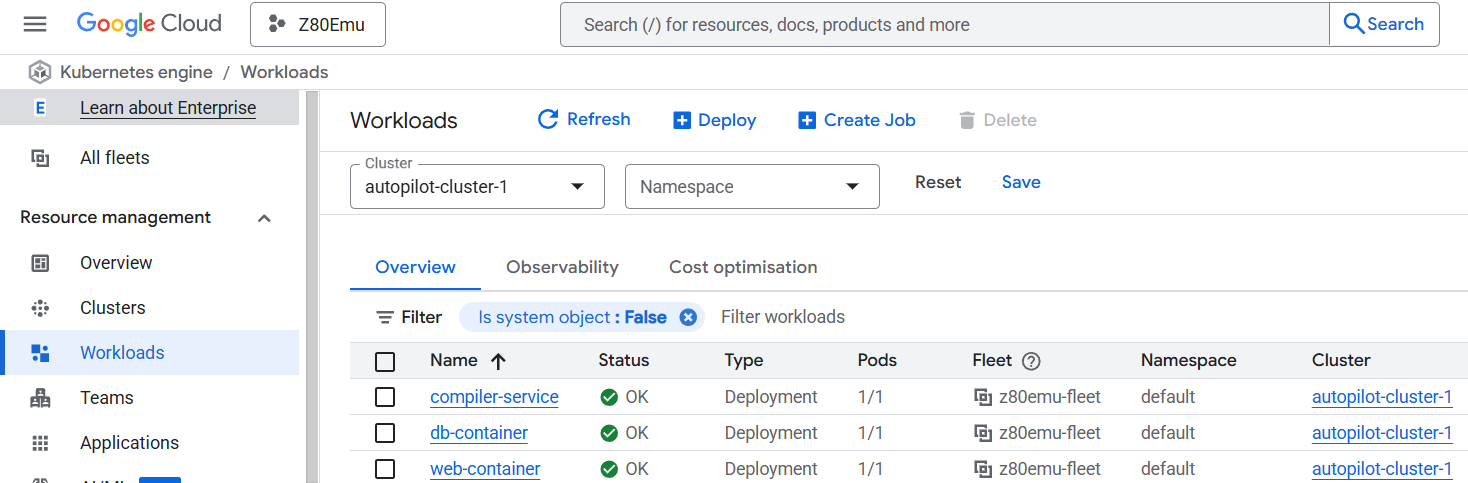
\includegraphics[width=0.8\textwidth]{images/googlecluster.png}
    \caption{Clusterul Kubernetes in Google Cloud Platform}
    \label{fig:googlecluster}
\end{figure}

\subsubsection{Domain}
Pentru a putea accesa aplicatia de pe internet, a fost achizitionat un domeniu \code{z80emu.online} prin platforma Spaceship. Acest domeniu a fost necesar pentru a putea accesa aplicatia de pe internet si pentru a putea folosi un certificat \code{SSL} generat de Google Cloud Platform. Acest domeniu este folosit pentru a accesa aplicatia in siguranta prin intermediul unui domeniu securizat, fara a fi nevoie sa se configureze manual certificatele \code{SSL} si redirectionarea traficului.

Un motiv datorita caruia Spaceship a fost ales pentru inregistrarea domeniului este faptul ca ofera un API simplu si usor de folosit pentru a gestiona domeniile. Acest lucru permite ca domeniul sa fie gestionat usor si rapid, fara a fi nevoie sa se acceseze manual platforma Spaceship. De asemenea, Spaceship ofera suport pentru \ac {DNS}, ceea ce permite ca domeniul sa fie configurat usor pentru a fi folosit cu Google Cloud Platform.

\subsection{CI/CD}

Pentru a putea implementa aplicatia in mod continuu si pentru a putea testa automat codul, s-a folosit GitHub Actions. Acesta permite ca codul sa fie testat automat la fiecare push si sa fie implementat automat in productie atunci cand este gata. Acest lucru permite ca aplicatia sa fie dezvoltata si testata rapid, fara a fi nevoie sa se faca manual teste sau implementari.

\subsubsection{Testarea librariei}
Un workflow de testare a fost creat pentru a testa libraria \code{z80emu-lib} la fiecare push. Acest workflow este definit in fisierul \code{.github/workflows/build.yml} si este folosit pentru a rula testele unitare ale librariei. In \cref{lst:libtestworkflow} este prezentat workflow-ul ce apelease \code{cargo test}. Acest workflow este declansat la fiecare push si la fiecare pull request. Acest lucru permite ca libraria sa fie testata automat si sa se asigure ca nu sunt introduse erori in codul sursa.
\begin{lstlisting}[language=yaml,caption={Workflow de testare a librariei},label={lst:libtestworkflow}]
on:
  push:
    branches: [ "master" ]
  pull_request:
    branches: [ "master" ]
jobs:
  build:
    runs-on: ubuntu-latest
    steps:
    - uses: actions/checkout@v4
      with:
        submodules: true
    - name: Build
      run: cargo build --verbose
    - name: Run tests
      run: cargo test --verbose
\end{lstlisting}

\begin{minipage}[c]{0.55\textwidth}
Datorita faptului ca fiecare commit de pe branchul \code{master} este testat automat, un utilizator care doreste sa foloseasca libraria va putea vedea chemarkul \cref{fig:libtestcheckmark} in pagina de GitHub a librariei, ceea ce indica faptul ca libraria a trecut toate testele si este stabila pentru a fi folosita. Acest lucru ofera un nivel suplimentar de incredere utilizatorilor care doresc sa foloseasca libraria in proiectele lor.
\end{minipage}
\hfill
\begin{minipage}[c]{0.4\textwidth}
    \centering
    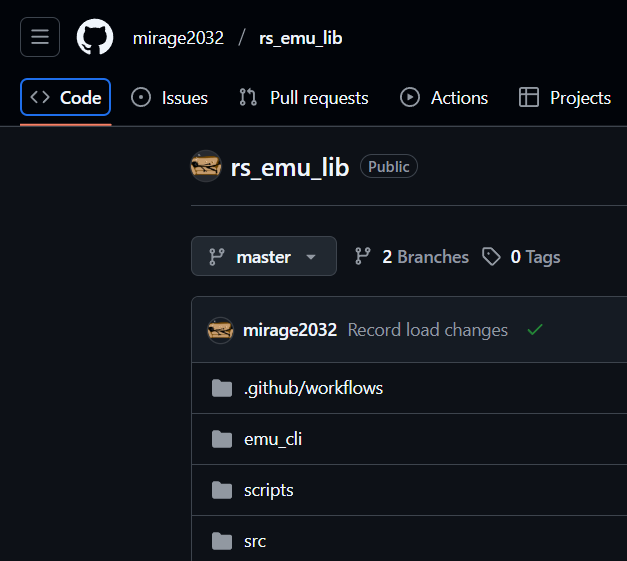
\includegraphics[width=\textwidth]{images/libtestcheckmark.png}
    \captionof{figure}{Workflow de testare a librariei}
    \label{fig:libtestcheckmark}
\end{minipage}

\subsubsection{Construirea imaginilor Docker}
Pentru a putea construi imaginile Docker ale aplicatiei, s-a folosit un workflow de GitHub Actions care este definit in fisierul \code{.github/workflows/dockerhub.yml}. Acest workflow este folosit pentru a construi imaginile Docker ale aplicatiei si pentru a le publica pe Docker Hub. In acest workflow \cref{lst:dockerhubworkflow} se poate observa cum pentru procesul de build, parametrii de setare ai cache-ului sunt setati pentru a folosi cache-ul de la GitHub Actions, ceea ce permite ca procesul de build sa fie mai rapid si mai eficient. De asemenea, se pot observa cum imaginile sunt etichetate cu versiunea scurta a commit-ului si cu \code{latest}, ceea ce permite ca imaginile sa fie usor de identificat si de folosit.

\begin{lstlisting}[language=yaml,caption={Workflow de construire a imaginilor Docker},label={lst:dockerhubworkflow}]
    steps:
      - name: Checkout repository
        uses: actions/checkout@v4

      - name: Log in to Docker Hub
        uses: docker/login-action@v3
        with:
          username: ${{ secrets.DOCKERHUB_USERNAME }}
          password: ${{ secrets.DOCKERHUB_TOKEN }}

      - name: Set up Docker Buildx
        uses: docker/setup-buildx-action@v3

      - name: Get short SHA
        run: echo "VERSION=$(git rev-parse --short HEAD)" >> $GITHUB_ENV

      - name: Build and run Z80 Emulator Web
        uses: docker/build-push-action@v6
        with:
          context: ./web
          push: true
          tags: |
            ${{ secrets.DOCKERHUB_USERNAME }}/z80emu:${{ env.VERSION }}
            ${{ secrets.DOCKERHUB_USERNAME }}/z80emu:latest
          cache-from: type=gha,scope=web
          cache-to: type=gha,mode=max,scope=web

      - name: Build and run Z80 Compiler Api
        uses: docker/build-push-action@v6
        with:
          context: ./ccompiler
          push: true
          tags: |
            ${{ secrets.DOCKERHUB_USERNAME }}/z80compiler-api:${{ env.VERSION }}
            ${{ secrets.DOCKERHUB_USERNAME }}/z80compiler-api:latest
          cache-from: type=gha,scope=ccompiler
          cache-to: type=gha,mode=max,scope=ccompiler

      - name: Build and run Z80 Emulator Database
        uses: docker/build-push-action@v6
        with:
          context: ./db
          push: true
          tags: |
            ${{ secrets.DOCKERHUB_USERNAME }}/z80emu-db:${{ env.VERSION }}
            ${{ secrets.DOCKERHUB_USERNAME }}/z80emu-db:latest
          cache-from: type=gha,scope=db
          cache-to: type=gha,mode=max,scope=db
\end{lstlisting}

\subsubsection{Deployment}
Acest workflow are ca scop crearea si resetarea clusterului \ac {K8s} in Google Cloud Platform. Acesta va folosi comanda \code{gcloud container clusters get-credentials} pentru a obtine credentialele clusterului si pentru a putea rula comenzi \code{kubectl} pe clusterul respectiv. In \cref{lst:k8sdeployworkflow} este prezentat workflow-ul de deployment al aplicatiei pe clusterul \ac {K8s}. Acest workflow va rula la fiecare push pe branchul \code{master} si va actualiza resursele din clusterul \ac {K8s} cu noile imagini Docker construite anterior. De asemenea, va reporni serviciile din cluster pentru a se asigura ca noile imagini sunt folosite.

\begin{lstlisting}[language=yaml,caption={Workflow deployment K8s},label={lst:k8sdeployworkflow}]
    steps:
      - name: Checkout code
        uses: actions/checkout@v4

      - name: Google Auth
        uses: 'google-github-actions/auth@v2'
        with:
          credentials_json: '${{ secrets.GOOGLE_CREDENTIALS }}'

      - name: Set up gcloud CLI
        uses: google-github-actions/setup-gcloud@v2
        with:
          project_id: z80emu-462619
          version: 'latest'

      - name: Install kubectl gcloud component
        run: gcloud components install kubectl

      - name: Get GKE credentials
        run: gcloud container clusters get-credentials \
         autopilot-cluster-1 --zone europe-north1 \
         --project z80emu-462619

      - name: Update Deployment
        run: |
          kubectl apply -f k8s/ccompiler
          kubectl apply -f k8s/db
          kubectl apply -f k8s/web

      - name: Restart # In case docketimage changes to get new one
        run: |
          kubectl rollout restart deployment web-container
          kubectl rollout restart deployment db-container
          kubectl rollout restart deployment compiler-service
\end{lstlisting}

\subsubsection{Update DNS}
Pentru a putea actualiza inregistrarile \ac {DNS} ale domeniului, s-a folosit un workflow de GitHub Actions care este definit in fisierul \code{.github/workflows/updatedns.yml}. Acest workflow este folosit pentru a actualiza inregistrarile \ac {DNS} ale domeniului la fiecare push pe branchul \code{master} si foloseste API-ul Spaceship pentru acest lucru. In \cref{lst:updatednsworkflow} este prezentat workflow-ul de actualizare a inregistrarilor \ac {DNS}. Acest workflow este programat sa ruleze la fiecare ora si va obtine adresa IP a serviciului \code{Ingress} din clusterul \ac {K8s} si o va actualiza inregistrarea \ac {DNS} a domeniului \code{z80emu.online}. Acest lucru permite ca domeniul sa fie actualizat automat cu adresa IP a serviciului, fara a fi nevoie sa se faca manual actualizari ale inregistrarilor \ac {DNS}.

\begin{lstlisting}[language=yaml,caption={Workflow de actualizare a inregistrarilor DNS},label={lst:updatednsworkflow}]
name: Update DNS Configuration

on:
  workflow_dispatch:  # Allows manual triggering
  schedule:
    - cron: '0 * * * *'  # Runs hourly (optional)

jobs:
  deploy:
    runs-on: ubuntu-latest
    steps:
      - name: Google Auth
        uses: 'google-github-actions/auth@v2'
        with:
          credentials_json: '${{ secrets.GOOGLE_CREDENTIALS }}'

      - name: Set up gcloud CLI
        uses: google-github-actions/setup-gcloud@v2
        with:
          project_id: z80emu-462619
          version: 'latest'

      - name: Get GKE credentials
        run: gcloud container clusters get-credentials \
         autopilot-cluster-1 --zone europe-north1 \
         --project z80emu-462619

      - name: Install kubectl gcloud component
        run: gcloud components install kubectl

      - name: Update Deployment
        env:
          SPACESHIP_KEY: ${{ secrets.SPACESHIP_KEY }}
          SPACESHIP_SECRET: ${{ secrets.SPACESHIP_SECRET }}
        run: |
          # Get IP and update DNS
          IP=$(kubectl get ingress z80emu-ingress \
           -o jsonpath='{.status.loadBalancer.ingress[0].ip}')
          curl -X PUT "https://spaceship.dev/api/v1/dns/records/z80emu.online" \
            -H "X-API-Key: ${SPACESHIP_KEY}" \
            -H "X-API-Secret: ${SPACESHIP_SECRET}" \
            -H "Content-Type: application/json" \
            -d '{
              "force": true,
              "items": [
                {
                  "type": "A",
                  "address": "'"${IP}"'",
                  "name": "@",
                  "ttl": 3600
                }
              ]
            }'
          echo "Updated DNS record with IP: ${IP}"
\end{lstlisting}

\clearpage
\section{Rezultate experimentale}
Pentru a testa capabilitatile aplicatiei, diferite programe au fost scrise in limbajul C, compilate si apoi rulate in emulatorul Z80. Aceste programe au fost folosite pentru a verifica daca aplicatia functioneaza corect si daca poate rula programe scrise in limbajul C. De asemenea, au fost testate si capabilitatile de formatare a codului sursa si de verificare a sintaxei.
Programul \code{rainbowclear.c} este un program simplu care va umple ecranul in mod continuu folosind culori diferite. Scopul acestui program este de a verifica compilarea, executarea programului cat si ecranul conectat la memoria emulatorlui. In \cref{lst:rainbowclearccode} se poate vedea codul sursa C al acestui program.

\begin{lstlisting}[language=C,caption={Cod sursa C pentru \code{rainbowclear.c}},label={lst:rainbowclearccode}]
char* DISPLAY=(char*)0x4000;
void main() {
    char color = 2;
    for(;;) {
        for(int i=0; i<0x6000; i++) {
            DISPLAY[i]=color;
        }
        color+=5;
    }
}
\end{lstlisting}

In timpul executiei acestui program \cref{fig:rainbowtestrun}, s-a facut observatia ca prin a pune un breakpoint la adresa de memorie \code{0x0030} unde se afla instructiunea \code{JR 0xDB}, executia programului va fi oprita fix dupa ce programul a terminat de umplut ecranul cu o culoare, marcand finalul unei iteratii a buclei exterioare.

\begin{figure}[H]
    \centering
    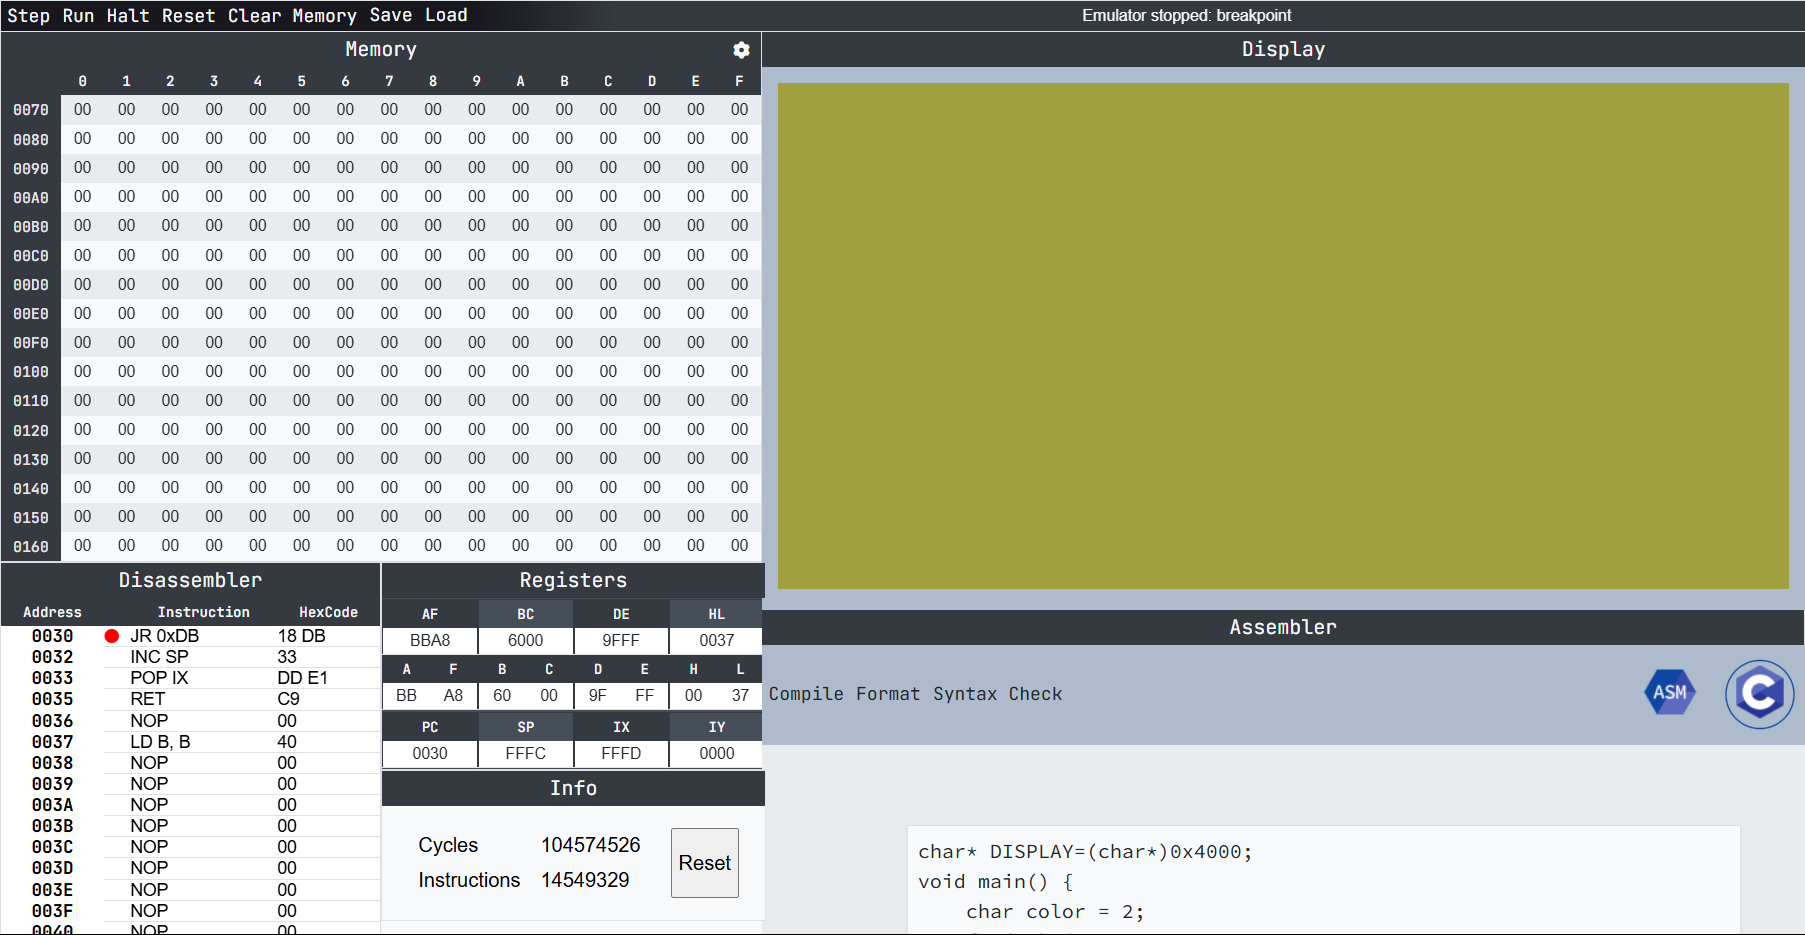
\includegraphics[width=0.8\textwidth]{images/rainbowtestrun.png}
    \caption{Testare program \code{rainbowclear.c}}
    \label{fig:rainbowtestrun}
\end{figure}

\clearpage
\section{Contributii}
In cadrul acestui proiect, au fost realizate mai multe contributii semnificative, atat in ceea ce priveste dezvoltarea aplicatiei, cat si in ceea ce priveste documentarea si testarea acesteia. Printre acestea se numara:
\begin{itemize}
    \item Implementarea unei librarii in Rust care sa ofere functionalitati de baza pentru un emulator Z80, cum ar fi emularea memoriei, a registrilor si a instructiunilor.
    \item Crearea unei aplicatii web folosind framework-ul Leptos, care sa permita utilizatorilor sa ruleze programe scrise in limbajul C pe un emulator Z80.
    \item Implementarea unui serviciu de compilare in Python care sa permita verificarea sintaxei si compilarea codului sursa in limbajul C.
    \item Crearea unei baze de date PostgreSQL pentru a stoca informatiile despre utilizatori si sesiunile acestora.
    \item Containerizarea aplicatiei folosind Docker si implementarea acesteia pe un cluster Kubernetes in Google Cloud Platform.
    \item Implementarea unui sistem de CI/CD folosind GitHub Actions pentru a testa automat codul si pentru a implementa aplicatia in productie.
\end{itemize}

\clearpage
\section{Bibliografie}
\printbibliography


\end{document}
